% for plotting
\documentclass[10pt]{article}
\usepackage{fullpage}
\usepackage{amsmath}    % for subequations
\usepackage{tikz}       % for generating figures with math symbols
\usepackage{graphicx}   % for figures
\usepackage{xcolor}
\usepackage{subfigure}  % for side-by-side figures

\begin{document}

\begin{figure}
  \begin{subfigure}
    \centering
    \resizebox{1.1\linewidth}{!}{% Created by tikzDevice version 0.12.3 on 2019-09-26 00:20:59
% !TEX encoding = UTF-8 Unicode
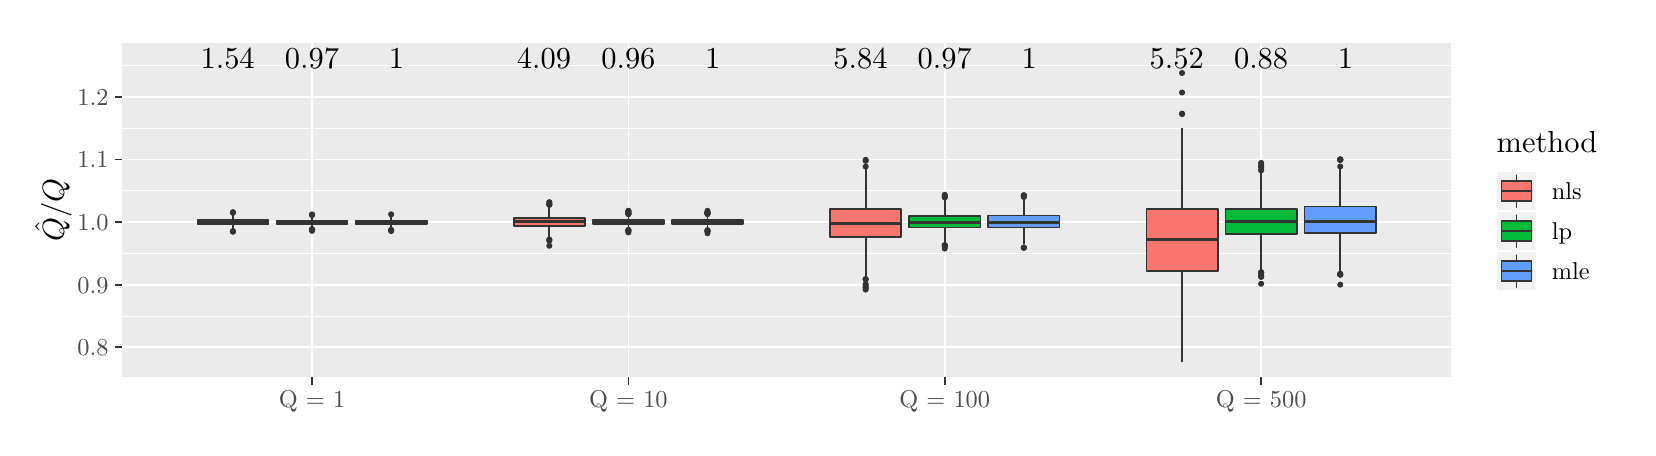
\begin{tikzpicture}[x=1pt,y=1pt]
\definecolor{fillColor}{RGB}{255,255,255}
\path[use as bounding box,fill=fillColor,fill opacity=0.00] (0,0) rectangle (578.16,144.54);
\begin{scope}
\path[clip] (  0.00,  0.00) rectangle (578.16,144.54);
\definecolor{drawColor}{RGB}{255,255,255}
\definecolor{fillColor}{RGB}{255,255,255}

\path[draw=drawColor,line width= 0.6pt,line join=round,line cap=round,fill=fillColor] (  0.00,  0.00) rectangle (578.16,144.54);
\end{scope}
\begin{scope}
\path[clip] ( 34.16, 18.22) rectangle (514.31,139.04);
\definecolor{fillColor}{gray}{0.92}

\path[fill=fillColor] ( 34.16, 18.22) rectangle (514.31,139.04);
\definecolor{drawColor}{RGB}{255,255,255}

\path[draw=drawColor,line width= 0.3pt,line join=round] ( 34.16, 40.36) --
	(514.31, 40.36);

\path[draw=drawColor,line width= 0.3pt,line join=round] ( 34.16, 62.97) --
	(514.31, 62.97);

\path[draw=drawColor,line width= 0.3pt,line join=round] ( 34.16, 85.57) --
	(514.31, 85.57);

\path[draw=drawColor,line width= 0.3pt,line join=round] ( 34.16,108.17) --
	(514.31,108.17);

\path[draw=drawColor,line width= 0.3pt,line join=round] ( 34.16,130.77) --
	(514.31,130.77);

\path[draw=drawColor,line width= 0.6pt,line join=round] ( 34.16, 29.06) --
	(514.31, 29.06);

\path[draw=drawColor,line width= 0.6pt,line join=round] ( 34.16, 51.67) --
	(514.31, 51.67);

\path[draw=drawColor,line width= 0.6pt,line join=round] ( 34.16, 74.27) --
	(514.31, 74.27);

\path[draw=drawColor,line width= 0.6pt,line join=round] ( 34.16, 96.87) --
	(514.31, 96.87);

\path[draw=drawColor,line width= 0.6pt,line join=round] ( 34.16,119.47) --
	(514.31,119.47);

\path[draw=drawColor,line width= 0.6pt,line join=round] (102.75, 18.22) --
	(102.75,139.04);

\path[draw=drawColor,line width= 0.6pt,line join=round] (217.07, 18.22) --
	(217.07,139.04);

\path[draw=drawColor,line width= 0.6pt,line join=round] (331.39, 18.22) --
	(331.39,139.04);

\path[draw=drawColor,line width= 0.6pt,line join=round] (445.71, 18.22) --
	(445.71,139.04);
\definecolor{drawColor}{gray}{0.20}
\definecolor{fillColor}{gray}{0.20}

\path[draw=drawColor,line width= 0.4pt,line join=round,line cap=round,fill=fillColor] ( 74.17, 77.90) circle (  0.89);

\path[draw=drawColor,line width= 0.4pt,line join=round,line cap=round,fill=fillColor] ( 74.17, 70.95) circle (  0.89);

\path[draw=drawColor,line width= 0.4pt,line join=round,line cap=round,fill=fillColor] ( 74.17, 70.81) circle (  0.89);

\path[draw=drawColor,line width= 0.4pt,line join=round,line cap=round,fill=fillColor] ( 74.17, 70.97) circle (  0.89);

\path[draw=drawColor,line width= 0.4pt,line join=round,line cap=round,fill=fillColor] ( 74.17, 77.62) circle (  0.89);

\path[draw=drawColor,line width= 0.6pt,line join=round] ( 74.17, 75.10) -- ( 74.17, 77.43);

\path[draw=drawColor,line width= 0.6pt,line join=round] ( 74.17, 73.46) -- ( 74.17, 71.17);
\definecolor{fillColor}{RGB}{248,118,109}

\path[draw=drawColor,line width= 0.6pt,line join=round,line cap=round,fill=fillColor] ( 61.31, 75.10) --
	( 61.31, 73.46) --
	( 87.03, 73.46) --
	( 87.03, 75.10) --
	( 61.31, 75.10) --
	cycle;

\path[draw=drawColor,line width= 1.1pt,line join=round] ( 61.31, 74.27) -- ( 87.03, 74.27);
\definecolor{fillColor}{gray}{0.20}

\path[draw=drawColor,line width= 0.4pt,line join=round,line cap=round,fill=fillColor] (102.75, 71.13) circle (  0.89);

\path[draw=drawColor,line width= 0.4pt,line join=round,line cap=round,fill=fillColor] (102.75, 76.78) circle (  0.89);

\path[draw=drawColor,line width= 0.4pt,line join=round,line cap=round,fill=fillColor] (102.75, 71.70) circle (  0.89);

\path[draw=drawColor,line width= 0.4pt,line join=round,line cap=round,fill=fillColor] (102.75, 71.55) circle (  0.89);

\path[draw=drawColor,line width= 0.4pt,line join=round,line cap=round,fill=fillColor] (102.75, 71.66) circle (  0.89);

\path[draw=drawColor,line width= 0.4pt,line join=round,line cap=round,fill=fillColor] (102.75, 71.46) circle (  0.89);

\path[draw=drawColor,line width= 0.4pt,line join=round,line cap=round,fill=fillColor] (102.75, 77.06) circle (  0.89);

\path[draw=drawColor,line width= 0.6pt,line join=round] (102.75, 74.90) -- (102.75, 76.73);

\path[draw=drawColor,line width= 0.6pt,line join=round] (102.75, 73.67) -- (102.75, 71.82);
\definecolor{fillColor}{RGB}{0,186,56}

\path[draw=drawColor,line width= 0.6pt,line join=round,line cap=round,fill=fillColor] ( 89.89, 74.90) --
	( 89.89, 73.67) --
	(115.61, 73.67) --
	(115.61, 74.90) --
	( 89.89, 74.90) --
	cycle;

\path[draw=drawColor,line width= 1.1pt,line join=round] ( 89.89, 74.29) -- (115.61, 74.29);
\definecolor{fillColor}{gray}{0.20}

\path[draw=drawColor,line width= 0.4pt,line join=round,line cap=round,fill=fillColor] (131.33, 71.03) circle (  0.89);

\path[draw=drawColor,line width= 0.4pt,line join=round,line cap=round,fill=fillColor] (131.33, 71.39) circle (  0.89);

\path[draw=drawColor,line width= 0.4pt,line join=round,line cap=round,fill=fillColor] (131.33, 71.47) circle (  0.89);

\path[draw=drawColor,line width= 0.4pt,line join=round,line cap=round,fill=fillColor] (131.33, 77.09) circle (  0.89);

\path[draw=drawColor,line width= 0.6pt,line join=round] (131.33, 74.91) -- (131.33, 76.89);

\path[draw=drawColor,line width= 0.6pt,line join=round] (131.33, 73.59) -- (131.33, 71.62);
\definecolor{fillColor}{RGB}{97,156,255}

\path[draw=drawColor,line width= 0.6pt,line join=round,line cap=round,fill=fillColor] (118.47, 74.91) --
	(118.47, 73.59) --
	(144.19, 73.59) --
	(144.19, 74.91) --
	(118.47, 74.91) --
	cycle;

\path[draw=drawColor,line width= 1.1pt,line join=round] (118.47, 74.27) -- (144.19, 74.27);
\definecolor{fillColor}{gray}{0.20}

\path[draw=drawColor,line width= 0.4pt,line join=round,line cap=round,fill=fillColor] (188.49, 80.55) circle (  0.89);

\path[draw=drawColor,line width= 0.4pt,line join=round,line cap=round,fill=fillColor] (188.49, 65.73) circle (  0.89);

\path[draw=drawColor,line width= 0.4pt,line join=round,line cap=round,fill=fillColor] (188.49, 81.28) circle (  0.89);

\path[draw=drawColor,line width= 0.4pt,line join=round,line cap=round,fill=fillColor] (188.49, 80.59) circle (  0.89);

\path[draw=drawColor,line width= 0.4pt,line join=round,line cap=round,fill=fillColor] (188.49, 67.86) circle (  0.89);

\path[draw=drawColor,line width= 0.4pt,line join=round,line cap=round,fill=fillColor] (188.49, 81.47) circle (  0.89);

\path[draw=drawColor,line width= 0.4pt,line join=round,line cap=round,fill=fillColor] (188.49, 67.52) circle (  0.89);

\path[draw=drawColor,line width= 0.4pt,line join=round,line cap=round,fill=fillColor] (188.49, 80.73) circle (  0.89);

\path[draw=drawColor,line width= 0.4pt,line join=round,line cap=round,fill=fillColor] (188.49, 67.96) circle (  0.89);

\path[draw=drawColor,line width= 0.6pt,line join=round] (188.49, 75.86) -- (188.49, 80.20);

\path[draw=drawColor,line width= 0.6pt,line join=round] (188.49, 72.79) -- (188.49, 68.22);
\definecolor{fillColor}{RGB}{248,118,109}

\path[draw=drawColor,line width= 0.6pt,line join=round,line cap=round,fill=fillColor] (175.63, 75.86) --
	(175.63, 72.79) --
	(201.35, 72.79) --
	(201.35, 75.86) --
	(175.63, 75.86) --
	cycle;

\path[draw=drawColor,line width= 1.1pt,line join=round] (175.63, 74.35) -- (201.35, 74.35);
\definecolor{fillColor}{gray}{0.20}

\path[draw=drawColor,line width= 0.4pt,line join=round,line cap=round,fill=fillColor] (217.07, 77.19) circle (  0.89);

\path[draw=drawColor,line width= 0.4pt,line join=round,line cap=round,fill=fillColor] (217.07, 77.40) circle (  0.89);

\path[draw=drawColor,line width= 0.4pt,line join=round,line cap=round,fill=fillColor] (217.07, 71.07) circle (  0.89);

\path[draw=drawColor,line width= 0.4pt,line join=round,line cap=round,fill=fillColor] (217.07, 77.44) circle (  0.89);

\path[draw=drawColor,line width= 0.4pt,line join=round,line cap=round,fill=fillColor] (217.07, 78.21) circle (  0.89);

\path[draw=drawColor,line width= 0.4pt,line join=round,line cap=round,fill=fillColor] (217.07, 71.21) circle (  0.89);

\path[draw=drawColor,line width= 0.4pt,line join=round,line cap=round,fill=fillColor] (217.07, 78.07) circle (  0.89);

\path[draw=drawColor,line width= 0.4pt,line join=round,line cap=round,fill=fillColor] (217.07, 77.22) circle (  0.89);

\path[draw=drawColor,line width= 0.4pt,line join=round,line cap=round,fill=fillColor] (217.07, 78.39) circle (  0.89);

\path[draw=drawColor,line width= 0.4pt,line join=round,line cap=round,fill=fillColor] (217.07, 77.31) circle (  0.89);

\path[draw=drawColor,line width= 0.4pt,line join=round,line cap=round,fill=fillColor] (217.07, 77.94) circle (  0.89);

\path[draw=drawColor,line width= 0.4pt,line join=round,line cap=round,fill=fillColor] (217.07, 71.45) circle (  0.89);

\path[draw=drawColor,line width= 0.4pt,line join=round,line cap=round,fill=fillColor] (217.07, 70.55) circle (  0.89);

\path[draw=drawColor,line width= 0.4pt,line join=round,line cap=round,fill=fillColor] (217.07, 71.39) circle (  0.89);

\path[draw=drawColor,line width= 0.6pt,line join=round] (217.07, 75.02) -- (217.07, 77.06);

\path[draw=drawColor,line width= 0.6pt,line join=round] (217.07, 73.61) -- (217.07, 71.49);
\definecolor{fillColor}{RGB}{0,186,56}

\path[draw=drawColor,line width= 0.6pt,line join=round,line cap=round,fill=fillColor] (204.21, 75.02) --
	(204.21, 73.61) --
	(229.93, 73.61) --
	(229.93, 75.02) --
	(204.21, 75.02) --
	cycle;

\path[draw=drawColor,line width= 1.1pt,line join=round] (204.21, 74.31) -- (229.93, 74.31);
\definecolor{fillColor}{gray}{0.20}

\path[draw=drawColor,line width= 0.4pt,line join=round,line cap=round,fill=fillColor] (245.65, 77.55) circle (  0.89);

\path[draw=drawColor,line width= 0.4pt,line join=round,line cap=round,fill=fillColor] (245.65, 70.97) circle (  0.89);

\path[draw=drawColor,line width= 0.4pt,line join=round,line cap=round,fill=fillColor] (245.65, 77.18) circle (  0.89);

\path[draw=drawColor,line width= 0.4pt,line join=round,line cap=round,fill=fillColor] (245.65, 77.78) circle (  0.89);

\path[draw=drawColor,line width= 0.4pt,line join=round,line cap=round,fill=fillColor] (245.65, 71.38) circle (  0.89);

\path[draw=drawColor,line width= 0.4pt,line join=round,line cap=round,fill=fillColor] (245.65, 77.77) circle (  0.89);

\path[draw=drawColor,line width= 0.4pt,line join=round,line cap=round,fill=fillColor] (245.65, 77.50) circle (  0.89);

\path[draw=drawColor,line width= 0.4pt,line join=round,line cap=round,fill=fillColor] (245.65, 78.36) circle (  0.89);

\path[draw=drawColor,line width= 0.4pt,line join=round,line cap=round,fill=fillColor] (245.65, 77.39) circle (  0.89);

\path[draw=drawColor,line width= 0.4pt,line join=round,line cap=round,fill=fillColor] (245.65, 77.31) circle (  0.89);

\path[draw=drawColor,line width= 0.4pt,line join=round,line cap=round,fill=fillColor] (245.65, 77.88) circle (  0.89);

\path[draw=drawColor,line width= 0.4pt,line join=round,line cap=round,fill=fillColor] (245.65, 71.14) circle (  0.89);

\path[draw=drawColor,line width= 0.4pt,line join=round,line cap=round,fill=fillColor] (245.65, 70.24) circle (  0.89);

\path[draw=drawColor,line width= 0.4pt,line join=round,line cap=round,fill=fillColor] (245.65, 71.01) circle (  0.89);

\path[draw=drawColor,line width= 0.4pt,line join=round,line cap=round,fill=fillColor] (245.65, 71.13) circle (  0.89);

\path[draw=drawColor,line width= 0.4pt,line join=round,line cap=round,fill=fillColor] (245.65, 71.19) circle (  0.89);

\path[draw=drawColor,line width= 0.4pt,line join=round,line cap=round,fill=fillColor] (245.65, 77.46) circle (  0.89);

\path[draw=drawColor,line width= 0.6pt,line join=round] (245.65, 74.99) -- (245.65, 76.99);

\path[draw=drawColor,line width= 0.6pt,line join=round] (245.65, 73.56) -- (245.65, 71.44);
\definecolor{fillColor}{RGB}{97,156,255}

\path[draw=drawColor,line width= 0.6pt,line join=round,line cap=round,fill=fillColor] (232.79, 74.99) --
	(232.79, 73.56) --
	(258.51, 73.56) --
	(258.51, 74.99) --
	(232.79, 74.99) --
	cycle;

\path[draw=drawColor,line width= 1.1pt,line join=round] (232.79, 74.27) -- (258.51, 74.27);
\definecolor{fillColor}{gray}{0.20}

\path[draw=drawColor,line width= 0.4pt,line join=round,line cap=round,fill=fillColor] (302.81, 50.54) circle (  0.89);

\path[draw=drawColor,line width= 0.4pt,line join=round,line cap=round,fill=fillColor] (302.81, 96.79) circle (  0.89);

\path[draw=drawColor,line width= 0.4pt,line join=round,line cap=round,fill=fillColor] (302.81, 49.91) circle (  0.89);

\path[draw=drawColor,line width= 0.4pt,line join=round,line cap=round,fill=fillColor] (302.81, 96.42) circle (  0.89);

\path[draw=drawColor,line width= 0.4pt,line join=round,line cap=round,fill=fillColor] (302.81, 94.34) circle (  0.89);

\path[draw=drawColor,line width= 0.4pt,line join=round,line cap=round,fill=fillColor] (302.81, 50.61) circle (  0.89);

\path[draw=drawColor,line width= 0.4pt,line join=round,line cap=round,fill=fillColor] (302.81, 51.40) circle (  0.89);

\path[draw=drawColor,line width= 0.4pt,line join=round,line cap=round,fill=fillColor] (302.81, 53.73) circle (  0.89);

\path[draw=drawColor,line width= 0.4pt,line join=round,line cap=round,fill=fillColor] (302.81, 51.83) circle (  0.89);

\path[draw=drawColor,line width= 0.4pt,line join=round,line cap=round,fill=fillColor] (302.81, 53.53) circle (  0.89);

\path[draw=drawColor,line width= 0.6pt,line join=round] (302.81, 78.95) -- (302.81, 93.86);

\path[draw=drawColor,line width= 0.6pt,line join=round] (302.81, 68.95) -- (302.81, 54.90);
\definecolor{fillColor}{RGB}{248,118,109}

\path[draw=drawColor,line width= 0.6pt,line join=round,line cap=round,fill=fillColor] (289.95, 78.95) --
	(289.95, 68.95) --
	(315.67, 68.95) --
	(315.67, 78.95) --
	(289.95, 78.95) --
	cycle;

\path[draw=drawColor,line width= 1.1pt,line join=round] (289.95, 73.66) -- (315.67, 73.66);
\definecolor{fillColor}{gray}{0.20}

\path[draw=drawColor,line width= 0.4pt,line join=round,line cap=round,fill=fillColor] (331.39, 83.45) circle (  0.89);

\path[draw=drawColor,line width= 0.4pt,line join=round,line cap=round,fill=fillColor] (331.39, 83.30) circle (  0.89);

\path[draw=drawColor,line width= 0.4pt,line join=round,line cap=round,fill=fillColor] (331.39, 65.85) circle (  0.89);

\path[draw=drawColor,line width= 0.4pt,line join=round,line cap=round,fill=fillColor] (331.39, 64.71) circle (  0.89);

\path[draw=drawColor,line width= 0.4pt,line join=round,line cap=round,fill=fillColor] (331.39, 83.25) circle (  0.89);

\path[draw=drawColor,line width= 0.4pt,line join=round,line cap=round,fill=fillColor] (331.39, 65.87) circle (  0.89);

\path[draw=drawColor,line width= 0.4pt,line join=round,line cap=round,fill=fillColor] (331.39, 83.84) circle (  0.89);

\path[draw=drawColor,line width= 0.4pt,line join=round,line cap=round,fill=fillColor] (331.39, 84.14) circle (  0.89);

\path[draw=drawColor,line width= 0.4pt,line join=round,line cap=round,fill=fillColor] (331.39, 65.36) circle (  0.89);

\path[draw=drawColor,line width= 0.4pt,line join=round,line cap=round,fill=fillColor] (331.39, 65.93) circle (  0.89);

\path[draw=drawColor,line width= 0.6pt,line join=round] (331.39, 76.46) -- (331.39, 82.29);

\path[draw=drawColor,line width= 0.6pt,line join=round] (331.39, 72.27) -- (331.39, 66.15);
\definecolor{fillColor}{RGB}{0,186,56}

\path[draw=drawColor,line width= 0.6pt,line join=round,line cap=round,fill=fillColor] (318.53, 76.46) --
	(318.53, 72.27) --
	(344.25, 72.27) --
	(344.25, 76.46) --
	(318.53, 76.46) --
	cycle;

\path[draw=drawColor,line width= 1.1pt,line join=round] (318.53, 74.24) -- (344.25, 74.24);
\definecolor{fillColor}{gray}{0.20}

\path[draw=drawColor,line width= 0.4pt,line join=round,line cap=round,fill=fillColor] (359.97, 83.94) circle (  0.89);

\path[draw=drawColor,line width= 0.4pt,line join=round,line cap=round,fill=fillColor] (359.97, 83.94) circle (  0.89);

\path[draw=drawColor,line width= 0.4pt,line join=round,line cap=round,fill=fillColor] (359.97, 65.07) circle (  0.89);

\path[draw=drawColor,line width= 0.4pt,line join=round,line cap=round,fill=fillColor] (359.97, 83.37) circle (  0.89);

\path[draw=drawColor,line width= 0.4pt,line join=round,line cap=round,fill=fillColor] (359.97, 64.98) circle (  0.89);

\path[draw=drawColor,line width= 0.4pt,line join=round,line cap=round,fill=fillColor] (359.97, 83.92) circle (  0.89);

\path[draw=drawColor,line width= 0.4pt,line join=round,line cap=round,fill=fillColor] (359.97, 83.50) circle (  0.89);

\path[draw=drawColor,line width= 0.4pt,line join=round,line cap=round,fill=fillColor] (359.97, 65.09) circle (  0.89);

\path[draw=drawColor,line width= 0.6pt,line join=round] (359.97, 76.62) -- (359.97, 82.60);

\path[draw=drawColor,line width= 0.6pt,line join=round] (359.97, 72.34) -- (359.97, 66.22);
\definecolor{fillColor}{RGB}{97,156,255}

\path[draw=drawColor,line width= 0.6pt,line join=round,line cap=round,fill=fillColor] (347.11, 76.62) --
	(347.11, 72.34) --
	(372.83, 72.34) --
	(372.83, 76.62) --
	(347.11, 76.62) --
	cycle;

\path[draw=drawColor,line width= 1.1pt,line join=round] (347.11, 74.27) -- (372.83, 74.27);
\definecolor{fillColor}{gray}{0.20}

\path[draw=drawColor,line width= 0.4pt,line join=round,line cap=round,fill=fillColor] (417.13,121.11) circle (  0.89);

\path[draw=drawColor,line width= 0.4pt,line join=round,line cap=round,fill=fillColor] (417.13,113.49) circle (  0.89);

\path[draw=drawColor,line width= 0.4pt,line join=round,line cap=round,fill=fillColor] (417.13,113.31) circle (  0.89);

\path[draw=drawColor,line width= 0.4pt,line join=round,line cap=round,fill=fillColor] (417.13,128.16) circle (  0.89);

\path[draw=drawColor,line width= 0.6pt,line join=round] (417.13, 78.95) -- (417.13,108.36);

\path[draw=drawColor,line width= 0.6pt,line join=round] (417.13, 56.70) -- (417.13, 23.71);
\definecolor{fillColor}{RGB}{248,118,109}

\path[draw=drawColor,line width= 0.6pt,line join=round,line cap=round,fill=fillColor] (404.27, 78.95) --
	(404.27, 56.70) --
	(430.00, 56.70) --
	(430.00, 78.95) --
	(404.27, 78.95) --
	cycle;

\path[draw=drawColor,line width= 1.1pt,line join=round] (404.27, 67.95) -- (430.00, 67.95);
\definecolor{fillColor}{gray}{0.20}

\path[draw=drawColor,line width= 0.4pt,line join=round,line cap=round,fill=fillColor] (445.71, 92.98) circle (  0.89);

\path[draw=drawColor,line width= 0.4pt,line join=round,line cap=round,fill=fillColor] (445.71, 52.00) circle (  0.89);

\path[draw=drawColor,line width= 0.4pt,line join=round,line cap=round,fill=fillColor] (445.71, 56.19) circle (  0.89);

\path[draw=drawColor,line width= 0.4pt,line join=round,line cap=round,fill=fillColor] (445.71, 54.48) circle (  0.89);

\path[draw=drawColor,line width= 0.4pt,line join=round,line cap=round,fill=fillColor] (445.71, 93.15) circle (  0.89);

\path[draw=drawColor,line width= 0.4pt,line join=round,line cap=round,fill=fillColor] (445.71, 95.68) circle (  0.89);

\path[draw=drawColor,line width= 0.4pt,line join=round,line cap=round,fill=fillColor] (445.71, 54.67) circle (  0.89);

\path[draw=drawColor,line width= 0.4pt,line join=round,line cap=round,fill=fillColor] (445.71, 94.21) circle (  0.89);

\path[draw=drawColor,line width= 0.4pt,line join=round,line cap=round,fill=fillColor] (445.71, 54.94) circle (  0.89);

\path[draw=drawColor,line width= 0.4pt,line join=round,line cap=round,fill=fillColor] (445.71, 94.90) circle (  0.89);

\path[draw=drawColor,line width= 0.4pt,line join=round,line cap=round,fill=fillColor] (445.71, 55.81) circle (  0.89);

\path[draw=drawColor,line width= 0.4pt,line join=round,line cap=round,fill=fillColor] (445.71, 94.35) circle (  0.89);

\path[draw=drawColor,line width= 0.4pt,line join=round,line cap=round,fill=fillColor] (445.71, 56.14) circle (  0.89);

\path[draw=drawColor,line width= 0.6pt,line join=round] (445.71, 79.05) -- (445.71, 92.46);

\path[draw=drawColor,line width= 0.6pt,line join=round] (445.71, 69.91) -- (445.71, 56.63);
\definecolor{fillColor}{RGB}{0,186,56}

\path[draw=drawColor,line width= 0.6pt,line join=round,line cap=round,fill=fillColor] (432.85, 79.05) --
	(432.85, 69.91) --
	(458.58, 69.91) --
	(458.58, 79.05) --
	(432.85, 79.05) --
	cycle;

\path[draw=drawColor,line width= 1.1pt,line join=round] (432.85, 74.54) -- (458.58, 74.54);
\definecolor{fillColor}{gray}{0.20}

\path[draw=drawColor,line width= 0.4pt,line join=round,line cap=round,fill=fillColor] (474.29, 96.90) circle (  0.89);

\path[draw=drawColor,line width= 0.4pt,line join=round,line cap=round,fill=fillColor] (474.29, 96.87) circle (  0.89);

\path[draw=drawColor,line width= 0.4pt,line join=round,line cap=round,fill=fillColor] (474.29, 51.67) circle (  0.89);

\path[draw=drawColor,line width= 0.4pt,line join=round,line cap=round,fill=fillColor] (474.29, 96.80) circle (  0.89);

\path[draw=drawColor,line width= 0.4pt,line join=round,line cap=round,fill=fillColor] (474.29, 96.79) circle (  0.89);

\path[draw=drawColor,line width= 0.4pt,line join=round,line cap=round,fill=fillColor] (474.29, 55.60) circle (  0.89);

\path[draw=drawColor,line width= 0.4pt,line join=round,line cap=round,fill=fillColor] (474.29, 55.32) circle (  0.89);

\path[draw=drawColor,line width= 0.4pt,line join=round,line cap=round,fill=fillColor] (474.29, 96.87) circle (  0.89);

\path[draw=drawColor,line width= 0.4pt,line join=round,line cap=round,fill=fillColor] (474.29, 55.30) circle (  0.89);

\path[draw=drawColor,line width= 0.4pt,line join=round,line cap=round,fill=fillColor] (474.29, 96.86) circle (  0.89);

\path[draw=drawColor,line width= 0.4pt,line join=round,line cap=round,fill=fillColor] (474.29, 55.40) circle (  0.89);

\path[draw=drawColor,line width= 0.4pt,line join=round,line cap=round,fill=fillColor] (474.29, 94.38) circle (  0.89);

\path[draw=drawColor,line width= 0.4pt,line join=round,line cap=round,fill=fillColor] (474.29, 55.40) circle (  0.89);

\path[draw=drawColor,line width= 0.4pt,line join=round,line cap=round,fill=fillColor] (474.29, 96.83) circle (  0.89);

\path[draw=drawColor,line width= 0.4pt,line join=round,line cap=round,fill=fillColor] (474.29, 96.84) circle (  0.89);

\path[draw=drawColor,line width= 0.4pt,line join=round,line cap=round,fill=fillColor] (474.29, 96.88) circle (  0.89);

\path[draw=drawColor,line width= 0.6pt,line join=round] (474.29, 79.91) -- (474.29, 93.89);

\path[draw=drawColor,line width= 0.6pt,line join=round] (474.29, 70.36) -- (474.29, 56.40);
\definecolor{fillColor}{RGB}{97,156,255}

\path[draw=drawColor,line width= 0.6pt,line join=round,line cap=round,fill=fillColor] (461.43, 79.91) --
	(461.43, 70.36) --
	(487.16, 70.36) --
	(487.16, 79.91) --
	(461.43, 79.91) --
	cycle;

\path[draw=drawColor,line width= 1.1pt,line join=round] (461.43, 74.34) -- (487.16, 74.34);
\definecolor{drawColor}{RGB}{0,0,0}

\node[text=drawColor,anchor=base,inner sep=0pt, outer sep=0pt, scale=  1.10] at (133.23,129.75) {1};

\node[text=drawColor,anchor=base,inner sep=0pt, outer sep=0pt, scale=  1.10] at (102.75,129.75) {0.97};

\node[text=drawColor,anchor=base,inner sep=0pt, outer sep=0pt, scale=  1.10] at ( 72.26,129.75) {1.54};

\node[text=drawColor,anchor=base,inner sep=0pt, outer sep=0pt, scale=  1.10] at (247.56,129.75) {1};

\node[text=drawColor,anchor=base,inner sep=0pt, outer sep=0pt, scale=  1.10] at (217.07,129.75) {0.96};

\node[text=drawColor,anchor=base,inner sep=0pt, outer sep=0pt, scale=  1.10] at (186.59,129.75) {4.09};

\node[text=drawColor,anchor=base,inner sep=0pt, outer sep=0pt, scale=  1.10] at (361.88,129.75) {1};

\node[text=drawColor,anchor=base,inner sep=0pt, outer sep=0pt, scale=  1.10] at (331.39,129.75) {0.97};

\node[text=drawColor,anchor=base,inner sep=0pt, outer sep=0pt, scale=  1.10] at (300.91,129.75) {5.84};

\node[text=drawColor,anchor=base,inner sep=0pt, outer sep=0pt, scale=  1.10] at (476.20,129.75) {1};

\node[text=drawColor,anchor=base,inner sep=0pt, outer sep=0pt, scale=  1.10] at (445.71,129.75) {0.88};

\node[text=drawColor,anchor=base,inner sep=0pt, outer sep=0pt, scale=  1.10] at (415.23,129.75) {5.52};
\end{scope}
\begin{scope}
\path[clip] (  0.00,  0.00) rectangle (578.16,144.54);
\definecolor{drawColor}{gray}{0.30}

\node[text=drawColor,anchor=base east,inner sep=0pt, outer sep=0pt, scale=  0.88] at ( 29.21, 26.03) {0.8};

\node[text=drawColor,anchor=base east,inner sep=0pt, outer sep=0pt, scale=  0.88] at ( 29.21, 48.64) {0.9};

\node[text=drawColor,anchor=base east,inner sep=0pt, outer sep=0pt, scale=  0.88] at ( 29.21, 71.24) {1.0};

\node[text=drawColor,anchor=base east,inner sep=0pt, outer sep=0pt, scale=  0.88] at ( 29.21, 93.84) {1.1};

\node[text=drawColor,anchor=base east,inner sep=0pt, outer sep=0pt, scale=  0.88] at ( 29.21,116.44) {1.2};
\end{scope}
\begin{scope}
\path[clip] (  0.00,  0.00) rectangle (578.16,144.54);
\definecolor{drawColor}{gray}{0.20}

\path[draw=drawColor,line width= 0.6pt,line join=round] ( 31.41, 29.06) --
	( 34.16, 29.06);

\path[draw=drawColor,line width= 0.6pt,line join=round] ( 31.41, 51.67) --
	( 34.16, 51.67);

\path[draw=drawColor,line width= 0.6pt,line join=round] ( 31.41, 74.27) --
	( 34.16, 74.27);

\path[draw=drawColor,line width= 0.6pt,line join=round] ( 31.41, 96.87) --
	( 34.16, 96.87);

\path[draw=drawColor,line width= 0.6pt,line join=round] ( 31.41,119.47) --
	( 34.16,119.47);
\end{scope}
\begin{scope}
\path[clip] (  0.00,  0.00) rectangle (578.16,144.54);
\definecolor{drawColor}{gray}{0.20}

\path[draw=drawColor,line width= 0.6pt,line join=round] (102.75, 15.47) --
	(102.75, 18.22);

\path[draw=drawColor,line width= 0.6pt,line join=round] (217.07, 15.47) --
	(217.07, 18.22);

\path[draw=drawColor,line width= 0.6pt,line join=round] (331.39, 15.47) --
	(331.39, 18.22);

\path[draw=drawColor,line width= 0.6pt,line join=round] (445.71, 15.47) --
	(445.71, 18.22);
\end{scope}
\begin{scope}
\path[clip] (  0.00,  0.00) rectangle (578.16,144.54);
\definecolor{drawColor}{gray}{0.30}

\node[text=drawColor,anchor=base,inner sep=0pt, outer sep=0pt, scale=  0.88] at (102.75,  7.21) {Q = 1};

\node[text=drawColor,anchor=base,inner sep=0pt, outer sep=0pt, scale=  0.88] at (217.07,  7.21) {Q = 10};

\node[text=drawColor,anchor=base,inner sep=0pt, outer sep=0pt, scale=  0.88] at (331.39,  7.21) {Q = 100};

\node[text=drawColor,anchor=base,inner sep=0pt, outer sep=0pt, scale=  0.88] at (445.71,  7.21) {Q = 500};
\end{scope}
\begin{scope}
\path[clip] (  0.00,  0.00) rectangle (578.16,144.54);
\definecolor{drawColor}{RGB}{0,0,0}

\node[text=drawColor,rotate= 90.00,anchor=base,inner sep=0pt, outer sep=0pt, scale=  1.10] at ( 13.08, 78.63) {$\hat{Q}/Q$};
\end{scope}
\begin{scope}
\path[clip] (  0.00,  0.00) rectangle (578.16,144.54);
\definecolor{fillColor}{RGB}{255,255,255}

\path[fill=fillColor] (525.31, 43.84) rectangle (572.66,113.42);
\end{scope}
\begin{scope}
\path[clip] (  0.00,  0.00) rectangle (578.16,144.54);
\definecolor{drawColor}{RGB}{0,0,0}

\node[text=drawColor,anchor=base west,inner sep=0pt, outer sep=0pt, scale=  1.10] at (530.81, 99.27) {method};
\end{scope}
\begin{scope}
\path[clip] (  0.00,  0.00) rectangle (578.16,144.54);
\definecolor{drawColor}{RGB}{255,255,255}
\definecolor{fillColor}{gray}{0.95}

\path[draw=drawColor,line width= 0.6pt,line join=round,line cap=round,fill=fillColor] (530.81, 78.25) rectangle (545.26, 92.70);
\end{scope}
\begin{scope}
\path[clip] (  0.00,  0.00) rectangle (578.16,144.54);
\definecolor{drawColor}{gray}{0.20}

\path[draw=drawColor,line width= 0.6pt,line join=round,line cap=round] (538.03, 79.70) --
	(538.03, 81.86);

\path[draw=drawColor,line width= 0.6pt,line join=round,line cap=round] (538.03, 89.09) --
	(538.03, 91.26);
\definecolor{fillColor}{RGB}{248,118,109}

\path[draw=drawColor,line width= 0.6pt,line join=round,line cap=round,fill=fillColor] (532.61, 81.86) rectangle (543.45, 89.09);

\path[draw=drawColor,line width= 0.6pt,line join=round,line cap=round] (532.61, 85.48) --
	(543.45, 85.48);
\end{scope}
\begin{scope}
\path[clip] (  0.00,  0.00) rectangle (578.16,144.54);
\definecolor{drawColor}{RGB}{255,255,255}
\definecolor{fillColor}{gray}{0.95}

\path[draw=drawColor,line width= 0.6pt,line join=round,line cap=round,fill=fillColor] (530.81, 63.80) rectangle (545.26, 78.25);
\end{scope}
\begin{scope}
\path[clip] (  0.00,  0.00) rectangle (578.16,144.54);
\definecolor{drawColor}{gray}{0.20}

\path[draw=drawColor,line width= 0.6pt,line join=round,line cap=round] (538.03, 65.24) --
	(538.03, 67.41);

\path[draw=drawColor,line width= 0.6pt,line join=round,line cap=round] (538.03, 74.64) --
	(538.03, 76.81);
\definecolor{fillColor}{RGB}{0,186,56}

\path[draw=drawColor,line width= 0.6pt,line join=round,line cap=round,fill=fillColor] (532.61, 67.41) rectangle (543.45, 74.64);

\path[draw=drawColor,line width= 0.6pt,line join=round,line cap=round] (532.61, 71.02) --
	(543.45, 71.02);
\end{scope}
\begin{scope}
\path[clip] (  0.00,  0.00) rectangle (578.16,144.54);
\definecolor{drawColor}{RGB}{255,255,255}
\definecolor{fillColor}{gray}{0.95}

\path[draw=drawColor,line width= 0.6pt,line join=round,line cap=round,fill=fillColor] (530.81, 49.34) rectangle (545.26, 63.80);
\end{scope}
\begin{scope}
\path[clip] (  0.00,  0.00) rectangle (578.16,144.54);
\definecolor{drawColor}{gray}{0.20}

\path[draw=drawColor,line width= 0.6pt,line join=round,line cap=round] (538.03, 50.79) --
	(538.03, 52.96);

\path[draw=drawColor,line width= 0.6pt,line join=round,line cap=round] (538.03, 60.18) --
	(538.03, 62.35);
\definecolor{fillColor}{RGB}{97,156,255}

\path[draw=drawColor,line width= 0.6pt,line join=round,line cap=round,fill=fillColor] (532.61, 52.96) rectangle (543.45, 60.18);

\path[draw=drawColor,line width= 0.6pt,line join=round,line cap=round] (532.61, 56.57) --
	(543.45, 56.57);
\end{scope}
\begin{scope}
\path[clip] (  0.00,  0.00) rectangle (578.16,144.54);
\definecolor{drawColor}{RGB}{0,0,0}

\node[text=drawColor,anchor=base west,inner sep=0pt, outer sep=0pt, scale=  0.88] at (550.76, 82.45) {nls};
\end{scope}
\begin{scope}
\path[clip] (  0.00,  0.00) rectangle (578.16,144.54);
\definecolor{drawColor}{RGB}{0,0,0}

\node[text=drawColor,anchor=base west,inner sep=0pt, outer sep=0pt, scale=  0.88] at (550.76, 67.99) {lp};
\end{scope}
\begin{scope}
\path[clip] (  0.00,  0.00) rectangle (578.16,144.54);
\definecolor{drawColor}{RGB}{0,0,0}

\node[text=drawColor,anchor=base west,inner sep=0pt, outer sep=0pt, scale=  0.88] at (550.76, 53.54) {mle};
\end{scope}
\end{tikzpicture}
}
  \end{subfigure}
  \hfill
  \begin{subfigure}
    \centering
    \resizebox{1.1\linewidth}{!}{% Created by tikzDevice version 0.12.3 on 2019-09-27 16:37:10
% !TEX encoding = UTF-8 Unicode
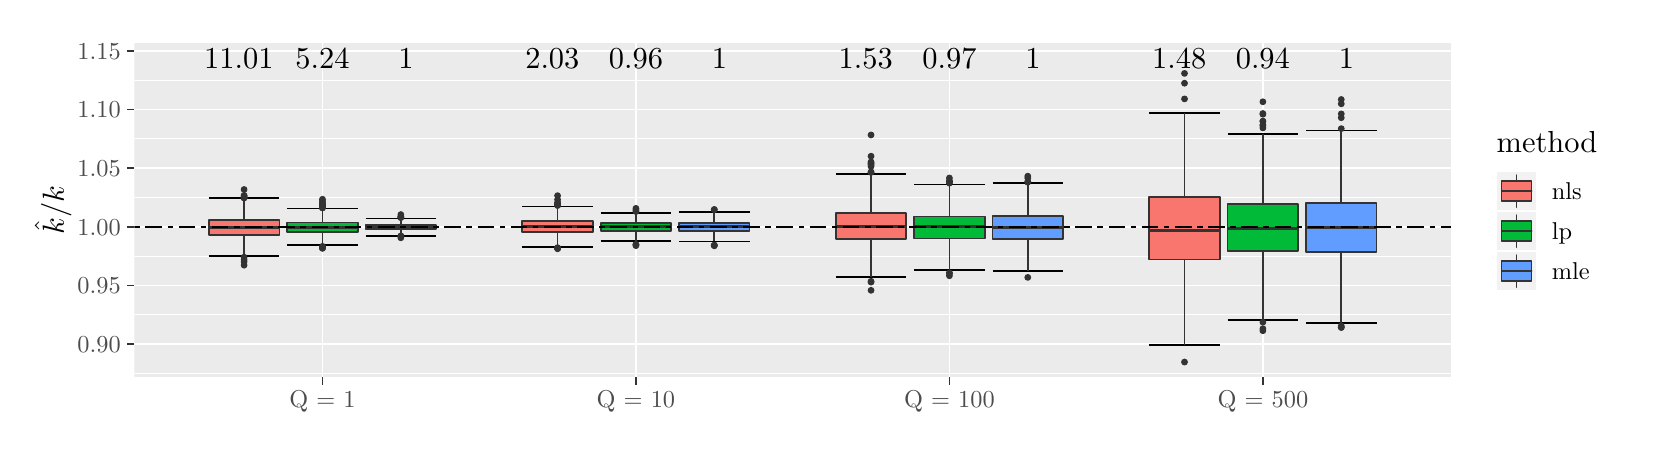
\begin{tikzpicture}[x=1pt,y=1pt]
\definecolor{fillColor}{RGB}{255,255,255}
\path[use as bounding box,fill=fillColor,fill opacity=0.00] (0,0) rectangle (578.16,144.54);
\begin{scope}
\path[clip] (  0.00,  0.00) rectangle (578.16,144.54);
\definecolor{drawColor}{RGB}{255,255,255}
\definecolor{fillColor}{RGB}{255,255,255}

\path[draw=drawColor,line width= 0.6pt,line join=round,line cap=round,fill=fillColor] (  0.00,  0.00) rectangle (578.16,144.54);
\end{scope}
\begin{scope}
\path[clip] ( 38.56, 18.22) rectangle (514.31,139.04);
\definecolor{fillColor}{gray}{0.92}

\path[fill=fillColor] ( 38.56, 18.22) rectangle (514.31,139.04);
\definecolor{drawColor}{RGB}{255,255,255}

\path[draw=drawColor,line width= 0.3pt,line join=round] ( 38.56, 19.64) --
	(514.31, 19.64);

\path[draw=drawColor,line width= 0.3pt,line join=round] ( 38.56, 40.82) --
	(514.31, 40.82);

\path[draw=drawColor,line width= 0.3pt,line join=round] ( 38.56, 62.00) --
	(514.31, 62.00);

\path[draw=drawColor,line width= 0.3pt,line join=round] ( 38.56, 83.18) --
	(514.31, 83.18);

\path[draw=drawColor,line width= 0.3pt,line join=round] ( 38.56,104.36) --
	(514.31,104.36);

\path[draw=drawColor,line width= 0.3pt,line join=round] ( 38.56,125.54) --
	(514.31,125.54);

\path[draw=drawColor,line width= 0.6pt,line join=round] ( 38.56, 30.23) --
	(514.31, 30.23);

\path[draw=drawColor,line width= 0.6pt,line join=round] ( 38.56, 51.41) --
	(514.31, 51.41);

\path[draw=drawColor,line width= 0.6pt,line join=round] ( 38.56, 72.59) --
	(514.31, 72.59);

\path[draw=drawColor,line width= 0.6pt,line join=round] ( 38.56, 93.77) --
	(514.31, 93.77);

\path[draw=drawColor,line width= 0.6pt,line join=round] ( 38.56,114.95) --
	(514.31,114.95);

\path[draw=drawColor,line width= 0.6pt,line join=round] ( 38.56,136.13) --
	(514.31,136.13);

\path[draw=drawColor,line width= 0.6pt,line join=round] (106.52, 18.22) --
	(106.52,139.04);

\path[draw=drawColor,line width= 0.6pt,line join=round] (219.79, 18.22) --
	(219.79,139.04);

\path[draw=drawColor,line width= 0.6pt,line join=round] (333.07, 18.22) --
	(333.07,139.04);

\path[draw=drawColor,line width= 0.6pt,line join=round] (446.34, 18.22) --
	(446.34,139.04);
\definecolor{drawColor}{RGB}{0,0,0}

\path[draw=drawColor,line width= 0.6pt,line join=round] ( 65.46, 82.89) --
	( 90.94, 82.89);

\path[draw=drawColor,line width= 0.6pt,line join=round] ( 78.20, 82.89) --
	( 78.20, 61.95);

\path[draw=drawColor,line width= 0.6pt,line join=round] ( 65.46, 61.95) --
	( 90.94, 61.95);

\path[draw=drawColor,line width= 0.6pt,line join=round] ( 93.78, 79.25) --
	(119.26, 79.25);

\path[draw=drawColor,line width= 0.6pt,line join=round] (106.52, 79.25) --
	(106.52, 66.05);

\path[draw=drawColor,line width= 0.6pt,line join=round] ( 93.78, 66.05) --
	(119.26, 66.05);

\path[draw=drawColor,line width= 0.6pt,line join=round] (122.09, 75.61) --
	(147.58, 75.61);

\path[draw=drawColor,line width= 0.6pt,line join=round] (134.84, 75.61) --
	(134.84, 69.37);

\path[draw=drawColor,line width= 0.6pt,line join=round] (122.09, 69.37) --
	(147.58, 69.37);

\path[draw=drawColor,line width= 0.6pt,line join=round] (178.73, 79.91) --
	(204.22, 79.91);

\path[draw=drawColor,line width= 0.6pt,line join=round] (191.48, 79.91) --
	(191.48, 65.19);

\path[draw=drawColor,line width= 0.6pt,line join=round] (178.73, 65.19) --
	(204.22, 65.19);

\path[draw=drawColor,line width= 0.6pt,line join=round] (207.05, 77.62) --
	(232.54, 77.62);

\path[draw=drawColor,line width= 0.6pt,line join=round] (219.79, 77.62) --
	(219.79, 67.35);

\path[draw=drawColor,line width= 0.6pt,line join=round] (207.05, 67.35) --
	(232.54, 67.35);

\path[draw=drawColor,line width= 0.6pt,line join=round] (235.37, 78.01) --
	(260.86, 78.01);

\path[draw=drawColor,line width= 0.6pt,line join=round] (248.11, 78.01) --
	(248.11, 67.30);

\path[draw=drawColor,line width= 0.6pt,line join=round] (235.37, 67.30) --
	(260.86, 67.30);

\path[draw=drawColor,line width= 0.6pt,line join=round] (292.01, 91.63) --
	(317.49, 91.63);

\path[draw=drawColor,line width= 0.6pt,line join=round] (304.75, 91.63) --
	(304.75, 54.53);

\path[draw=drawColor,line width= 0.6pt,line join=round] (292.01, 54.53) --
	(317.49, 54.53);

\path[draw=drawColor,line width= 0.6pt,line join=round] (320.33, 87.92) --
	(345.81, 87.92);

\path[draw=drawColor,line width= 0.6pt,line join=round] (333.07, 87.92) --
	(333.07, 57.05);

\path[draw=drawColor,line width= 0.6pt,line join=round] (320.33, 57.05) --
	(345.81, 57.05);

\path[draw=drawColor,line width= 0.6pt,line join=round] (348.64, 88.38) --
	(374.13, 88.38);

\path[draw=drawColor,line width= 0.6pt,line join=round] (361.39, 88.38) --
	(361.39, 56.65);

\path[draw=drawColor,line width= 0.6pt,line join=round] (348.64, 56.65) --
	(374.13, 56.65);

\path[draw=drawColor,line width= 0.6pt,line join=round] (405.28,113.69) --
	(430.77,113.69);

\path[draw=drawColor,line width= 0.6pt,line join=round] (418.02,113.69) --
	(418.02, 29.78);

\path[draw=drawColor,line width= 0.6pt,line join=round] (405.28, 29.78) --
	(430.77, 29.78);

\path[draw=drawColor,line width= 0.6pt,line join=round] (433.60,106.06) --
	(459.09,106.06);

\path[draw=drawColor,line width= 0.6pt,line join=round] (446.34,106.06) --
	(446.34, 38.85);

\path[draw=drawColor,line width= 0.6pt,line join=round] (433.60, 38.85) --
	(459.09, 38.85);

\path[draw=drawColor,line width= 0.6pt,line join=round] (461.92,107.44) --
	(487.40,107.44);

\path[draw=drawColor,line width= 0.6pt,line join=round] (474.66,107.44) --
	(474.66, 37.76);

\path[draw=drawColor,line width= 0.6pt,line join=round] (461.92, 37.76) --
	(487.40, 37.76);
\definecolor{drawColor}{gray}{0.20}
\definecolor{fillColor}{gray}{0.20}

\path[draw=drawColor,line width= 0.4pt,line join=round,line cap=round,fill=fillColor] ( 78.20, 58.72) circle (  1.02);

\path[draw=drawColor,line width= 0.4pt,line join=round,line cap=round,fill=fillColor] ( 78.20, 83.11) circle (  1.02);

\path[draw=drawColor,line width= 0.4pt,line join=round,line cap=round,fill=fillColor] ( 78.20, 83.79) circle (  1.02);

\path[draw=drawColor,line width= 0.4pt,line join=round,line cap=round,fill=fillColor] ( 78.20, 83.06) circle (  1.02);

\path[draw=drawColor,line width= 0.4pt,line join=round,line cap=round,fill=fillColor] ( 78.20, 83.40) circle (  1.02);

\path[draw=drawColor,line width= 0.4pt,line join=round,line cap=round,fill=fillColor] ( 78.20, 61.62) circle (  1.02);

\path[draw=drawColor,line width= 0.4pt,line join=round,line cap=round,fill=fillColor] ( 78.20, 86.06) circle (  1.02);

\path[draw=drawColor,line width= 0.4pt,line join=round,line cap=round,fill=fillColor] ( 78.20, 83.05) circle (  1.02);

\path[draw=drawColor,line width= 0.4pt,line join=round,line cap=round,fill=fillColor] ( 78.20, 60.72) circle (  1.02);

\path[draw=drawColor,line width= 0.4pt,line join=round,line cap=round,fill=fillColor] ( 78.20, 59.94) circle (  1.02);

\path[draw=drawColor,line width= 0.4pt,line join=round,line cap=round,fill=fillColor] ( 78.20, 83.92) circle (  1.02);

\path[draw=drawColor,line width= 0.6pt,line join=round] ( 78.20, 75.01) -- ( 78.20, 82.89);

\path[draw=drawColor,line width= 0.6pt,line join=round] ( 78.20, 69.73) -- ( 78.20, 61.95);
\definecolor{fillColor}{RGB}{248,118,109}

\path[draw=drawColor,line width= 0.6pt,line join=round,line cap=round,fill=fillColor] ( 65.46, 75.01) --
	( 65.46, 69.73) --
	( 90.94, 69.73) --
	( 90.94, 75.01) --
	( 65.46, 75.01) --
	cycle;

\path[draw=drawColor,line width= 1.1pt,line join=round] ( 65.46, 72.35) -- ( 90.94, 72.35);
\definecolor{fillColor}{gray}{0.20}

\path[draw=drawColor,line width= 0.4pt,line join=round,line cap=round,fill=fillColor] (106.52, 79.83) circle (  1.02);

\path[draw=drawColor,line width= 0.4pt,line join=round,line cap=round,fill=fillColor] (106.52, 79.53) circle (  1.02);

\path[draw=drawColor,line width= 0.4pt,line join=round,line cap=round,fill=fillColor] (106.52, 64.90) circle (  1.02);

\path[draw=drawColor,line width= 0.4pt,line join=round,line cap=round,fill=fillColor] (106.52, 64.83) circle (  1.02);

\path[draw=drawColor,line width= 0.4pt,line join=round,line cap=round,fill=fillColor] (106.52, 81.94) circle (  1.02);

\path[draw=drawColor,line width= 0.4pt,line join=round,line cap=round,fill=fillColor] (106.52, 79.39) circle (  1.02);

\path[draw=drawColor,line width= 0.4pt,line join=round,line cap=round,fill=fillColor] (106.52, 79.97) circle (  1.02);

\path[draw=drawColor,line width= 0.4pt,line join=round,line cap=round,fill=fillColor] (106.52, 81.14) circle (  1.02);

\path[draw=drawColor,line width= 0.4pt,line join=round,line cap=round,fill=fillColor] (106.52, 79.55) circle (  1.02);

\path[draw=drawColor,line width= 0.4pt,line join=round,line cap=round,fill=fillColor] (106.52, 65.51) circle (  1.02);

\path[draw=drawColor,line width= 0.4pt,line join=round,line cap=round,fill=fillColor] (106.52, 79.69) circle (  1.02);

\path[draw=drawColor,line width= 0.4pt,line join=round,line cap=round,fill=fillColor] (106.52, 80.25) circle (  1.02);

\path[draw=drawColor,line width= 0.4pt,line join=round,line cap=round,fill=fillColor] (106.52, 80.32) circle (  1.02);

\path[draw=drawColor,line width= 0.4pt,line join=round,line cap=round,fill=fillColor] (106.52, 81.14) circle (  1.02);

\path[draw=drawColor,line width= 0.4pt,line join=round,line cap=round,fill=fillColor] (106.52, 80.74) circle (  1.02);

\path[draw=drawColor,line width= 0.4pt,line join=round,line cap=round,fill=fillColor] (106.52, 82.53) circle (  1.02);

\path[draw=drawColor,line width= 0.4pt,line join=round,line cap=round,fill=fillColor] (106.52, 65.22) circle (  1.02);

\path[draw=drawColor,line width= 0.4pt,line join=round,line cap=round,fill=fillColor] (106.52, 65.33) circle (  1.02);

\path[draw=drawColor,line width= 0.4pt,line join=round,line cap=round,fill=fillColor] (106.52, 64.92) circle (  1.02);

\path[draw=drawColor,line width= 0.6pt,line join=round] (106.52, 74.17) -- (106.52, 79.25);

\path[draw=drawColor,line width= 0.6pt,line join=round] (106.52, 70.73) -- (106.52, 66.05);
\definecolor{fillColor}{RGB}{0,186,56}

\path[draw=drawColor,line width= 0.6pt,line join=round,line cap=round,fill=fillColor] ( 93.78, 74.17) --
	( 93.78, 70.73) --
	(119.26, 70.73) --
	(119.26, 74.17) --
	( 93.78, 74.17) --
	cycle;

\path[draw=drawColor,line width= 1.1pt,line join=round] ( 93.78, 72.49) -- (119.26, 72.49);
\definecolor{fillColor}{gray}{0.20}

\path[draw=drawColor,line width= 0.4pt,line join=round,line cap=round,fill=fillColor] (134.84, 76.16) circle (  1.02);

\path[draw=drawColor,line width= 0.4pt,line join=round,line cap=round,fill=fillColor] (134.84, 77.00) circle (  1.02);

\path[draw=drawColor,line width= 0.4pt,line join=round,line cap=round,fill=fillColor] (134.84, 75.89) circle (  1.02);

\path[draw=drawColor,line width= 0.4pt,line join=round,line cap=round,fill=fillColor] (134.84, 76.28) circle (  1.02);

\path[draw=drawColor,line width= 0.4pt,line join=round,line cap=round,fill=fillColor] (134.84, 69.27) circle (  1.02);

\path[draw=drawColor,line width= 0.4pt,line join=round,line cap=round,fill=fillColor] (134.84, 68.61) circle (  1.02);

\path[draw=drawColor,line width= 0.4pt,line join=round,line cap=round,fill=fillColor] (134.84, 69.18) circle (  1.02);

\path[draw=drawColor,line width= 0.4pt,line join=round,line cap=round,fill=fillColor] (134.84, 76.06) circle (  1.02);

\path[draw=drawColor,line width= 0.6pt,line join=round] (134.84, 73.26) -- (134.84, 75.61);

\path[draw=drawColor,line width= 0.6pt,line join=round] (134.84, 71.67) -- (134.84, 69.37);
\definecolor{fillColor}{RGB}{97,156,255}

\path[draw=drawColor,line width= 0.6pt,line join=round,line cap=round,fill=fillColor] (122.09, 73.26) --
	(122.09, 71.67) --
	(147.58, 71.67) --
	(147.58, 73.26) --
	(122.09, 73.26) --
	cycle;

\path[draw=drawColor,line width= 1.1pt,line join=round] (122.09, 72.44) -- (147.58, 72.44);
\definecolor{fillColor}{gray}{0.20}

\path[draw=drawColor,line width= 0.4pt,line join=round,line cap=round,fill=fillColor] (191.48, 80.48) circle (  1.02);

\path[draw=drawColor,line width= 0.4pt,line join=round,line cap=round,fill=fillColor] (191.48, 64.85) circle (  1.02);

\path[draw=drawColor,line width= 0.4pt,line join=round,line cap=round,fill=fillColor] (191.48, 83.84) circle (  1.02);

\path[draw=drawColor,line width= 0.4pt,line join=round,line cap=round,fill=fillColor] (191.48, 80.62) circle (  1.02);

\path[draw=drawColor,line width= 0.4pt,line join=round,line cap=round,fill=fillColor] (191.48, 64.65) circle (  1.02);

\path[draw=drawColor,line width= 0.4pt,line join=round,line cap=round,fill=fillColor] (191.48, 64.88) circle (  1.02);

\path[draw=drawColor,line width= 0.4pt,line join=round,line cap=round,fill=fillColor] (191.48, 64.97) circle (  1.02);

\path[draw=drawColor,line width= 0.4pt,line join=round,line cap=round,fill=fillColor] (191.48, 82.42) circle (  1.02);

\path[draw=drawColor,line width= 0.4pt,line join=round,line cap=round,fill=fillColor] (191.48, 81.42) circle (  1.02);

\path[draw=drawColor,line width= 0.4pt,line join=round,line cap=round,fill=fillColor] (191.48, 80.92) circle (  1.02);

\path[draw=drawColor,line width= 0.4pt,line join=round,line cap=round,fill=fillColor] (191.48, 80.30) circle (  1.02);

\path[draw=drawColor,line width= 0.4pt,line join=round,line cap=round,fill=fillColor] (191.48, 80.36) circle (  1.02);

\path[draw=drawColor,line width= 0.4pt,line join=round,line cap=round,fill=fillColor] (191.48, 64.99) circle (  1.02);

\path[draw=drawColor,line width= 0.6pt,line join=round] (191.48, 74.57) -- (191.48, 79.91);

\path[draw=drawColor,line width= 0.6pt,line join=round] (191.48, 70.78) -- (191.48, 65.19);
\definecolor{fillColor}{RGB}{248,118,109}

\path[draw=drawColor,line width= 0.6pt,line join=round,line cap=round,fill=fillColor] (178.73, 74.57) --
	(178.73, 70.78) --
	(204.22, 70.78) --
	(204.22, 74.57) --
	(178.73, 74.57) --
	cycle;

\path[draw=drawColor,line width= 1.1pt,line join=round] (178.73, 72.52) -- (204.22, 72.52);
\definecolor{fillColor}{gray}{0.20}

\path[draw=drawColor,line width= 0.4pt,line join=round,line cap=round,fill=fillColor] (219.79, 66.18) circle (  1.02);

\path[draw=drawColor,line width= 0.4pt,line join=round,line cap=round,fill=fillColor] (219.79, 66.20) circle (  1.02);

\path[draw=drawColor,line width= 0.4pt,line join=round,line cap=round,fill=fillColor] (219.79, 65.77) circle (  1.02);

\path[draw=drawColor,line width= 0.4pt,line join=round,line cap=round,fill=fillColor] (219.79, 78.10) circle (  1.02);

\path[draw=drawColor,line width= 0.4pt,line join=round,line cap=round,fill=fillColor] (219.79, 79.25) circle (  1.02);

\path[draw=drawColor,line width= 0.4pt,line join=round,line cap=round,fill=fillColor] (219.79, 78.65) circle (  1.02);

\path[draw=drawColor,line width= 0.6pt,line join=round] (219.79, 73.90) -- (219.79, 77.62);

\path[draw=drawColor,line width= 0.6pt,line join=round] (219.79, 71.15) -- (219.79, 67.35);
\definecolor{fillColor}{RGB}{0,186,56}

\path[draw=drawColor,line width= 0.6pt,line join=round,line cap=round,fill=fillColor] (207.05, 73.90) --
	(207.05, 71.15) --
	(232.54, 71.15) --
	(232.54, 73.90) --
	(207.05, 73.90) --
	cycle;

\path[draw=drawColor,line width= 1.1pt,line join=round] (207.05, 72.52) -- (232.54, 72.52);
\definecolor{fillColor}{gray}{0.20}

\path[draw=drawColor,line width= 0.4pt,line join=round,line cap=round,fill=fillColor] (248.11, 65.93) circle (  1.02);

\path[draw=drawColor,line width= 0.4pt,line join=round,line cap=round,fill=fillColor] (248.11, 65.92) circle (  1.02);

\path[draw=drawColor,line width= 0.4pt,line join=round,line cap=round,fill=fillColor] (248.11, 65.72) circle (  1.02);

\path[draw=drawColor,line width= 0.4pt,line join=round,line cap=round,fill=fillColor] (248.11, 78.80) circle (  1.02);

\path[draw=drawColor,line width= 0.4pt,line join=round,line cap=round,fill=fillColor] (248.11, 78.82) circle (  1.02);

\path[draw=drawColor,line width= 0.6pt,line join=round] (248.11, 73.93) -- (248.11, 78.01);

\path[draw=drawColor,line width= 0.6pt,line join=round] (248.11, 71.15) -- (248.11, 67.30);
\definecolor{fillColor}{RGB}{97,156,255}

\path[draw=drawColor,line width= 0.6pt,line join=round,line cap=round,fill=fillColor] (235.37, 73.93) --
	(235.37, 71.15) --
	(260.86, 71.15) --
	(260.86, 73.93) --
	(235.37, 73.93) --
	cycle;

\path[draw=drawColor,line width= 1.1pt,line join=round] (235.37, 72.58) -- (260.86, 72.58);
\definecolor{fillColor}{gray}{0.20}

\path[draw=drawColor,line width= 0.4pt,line join=round,line cap=round,fill=fillColor] (304.75, 95.30) circle (  1.02);

\path[draw=drawColor,line width= 0.4pt,line join=round,line cap=round,fill=fillColor] (304.75, 96.02) circle (  1.02);

\path[draw=drawColor,line width= 0.4pt,line join=round,line cap=round,fill=fillColor] (304.75, 92.24) circle (  1.02);

\path[draw=drawColor,line width= 0.4pt,line join=round,line cap=round,fill=fillColor] (304.75, 52.89) circle (  1.02);

\path[draw=drawColor,line width= 0.4pt,line join=round,line cap=round,fill=fillColor] (304.75,105.77) circle (  1.02);

\path[draw=drawColor,line width= 0.4pt,line join=round,line cap=round,fill=fillColor] (304.75, 98.09) circle (  1.02);

\path[draw=drawColor,line width= 0.4pt,line join=round,line cap=round,fill=fillColor] (304.75, 92.39) circle (  1.02);

\path[draw=drawColor,line width= 0.4pt,line join=round,line cap=round,fill=fillColor] (304.75, 49.63) circle (  1.02);

\path[draw=drawColor,line width= 0.4pt,line join=round,line cap=round,fill=fillColor] (304.75, 94.97) circle (  1.02);

\path[draw=drawColor,line width= 0.4pt,line join=round,line cap=round,fill=fillColor] (304.75, 94.41) circle (  1.02);

\path[draw=drawColor,line width= 0.4pt,line join=round,line cap=round,fill=fillColor] (304.75, 52.58) circle (  1.02);

\path[draw=drawColor,line width= 0.4pt,line join=round,line cap=round,fill=fillColor] (304.75, 95.69) circle (  1.02);

\path[draw=drawColor,line width= 0.6pt,line join=round] (304.75, 77.68) -- (304.75, 91.63);

\path[draw=drawColor,line width= 0.6pt,line join=round] (304.75, 68.10) -- (304.75, 54.53);
\definecolor{fillColor}{RGB}{248,118,109}

\path[draw=drawColor,line width= 0.6pt,line join=round,line cap=round,fill=fillColor] (292.01, 77.68) --
	(292.01, 68.10) --
	(317.49, 68.10) --
	(317.49, 77.68) --
	(292.01, 77.68) --
	cycle;

\path[draw=drawColor,line width= 1.1pt,line join=round] (292.01, 72.84) -- (317.49, 72.84);
\definecolor{fillColor}{gray}{0.20}

\path[draw=drawColor,line width= 0.4pt,line join=round,line cap=round,fill=fillColor] (333.07, 55.96) circle (  1.02);

\path[draw=drawColor,line width= 0.4pt,line join=round,line cap=round,fill=fillColor] (333.07, 88.84) circle (  1.02);

\path[draw=drawColor,line width= 0.4pt,line join=round,line cap=round,fill=fillColor] (333.07, 90.22) circle (  1.02);

\path[draw=drawColor,line width= 0.4pt,line join=round,line cap=round,fill=fillColor] (333.07, 89.22) circle (  1.02);

\path[draw=drawColor,line width= 0.4pt,line join=round,line cap=round,fill=fillColor] (333.07, 55.74) circle (  1.02);

\path[draw=drawColor,line width= 0.4pt,line join=round,line cap=round,fill=fillColor] (333.07, 54.90) circle (  1.02);

\path[draw=drawColor,line width= 0.4pt,line join=round,line cap=round,fill=fillColor] (333.07, 88.85) circle (  1.02);

\path[draw=drawColor,line width= 0.4pt,line join=round,line cap=round,fill=fillColor] (333.07, 88.35) circle (  1.02);

\path[draw=drawColor,line width= 0.6pt,line join=round] (333.07, 76.25) -- (333.07, 87.92);

\path[draw=drawColor,line width= 0.6pt,line join=round] (333.07, 68.38) -- (333.07, 57.05);
\definecolor{fillColor}{RGB}{0,186,56}

\path[draw=drawColor,line width= 0.6pt,line join=round,line cap=round,fill=fillColor] (320.33, 76.25) --
	(320.33, 68.38) --
	(345.81, 68.38) --
	(345.81, 76.25) --
	(320.33, 76.25) --
	cycle;

\path[draw=drawColor,line width= 1.1pt,line join=round] (320.33, 72.64) -- (345.81, 72.64);
\definecolor{fillColor}{gray}{0.20}

\path[draw=drawColor,line width= 0.4pt,line join=round,line cap=round,fill=fillColor] (361.39, 90.89) circle (  1.02);

\path[draw=drawColor,line width= 0.4pt,line join=round,line cap=round,fill=fillColor] (361.39, 90.19) circle (  1.02);

\path[draw=drawColor,line width= 0.4pt,line join=round,line cap=round,fill=fillColor] (361.39, 54.30) circle (  1.02);

\path[draw=drawColor,line width= 0.4pt,line join=round,line cap=round,fill=fillColor] (361.39, 88.90) circle (  1.02);

\path[draw=drawColor,line width= 0.4pt,line join=round,line cap=round,fill=fillColor] (361.39, 88.70) circle (  1.02);

\path[draw=drawColor,line width= 0.6pt,line join=round] (361.39, 76.42) -- (361.39, 88.38);

\path[draw=drawColor,line width= 0.6pt,line join=round] (361.39, 68.25) -- (361.39, 56.65);
\definecolor{fillColor}{RGB}{97,156,255}

\path[draw=drawColor,line width= 0.6pt,line join=round,line cap=round,fill=fillColor] (348.64, 76.42) --
	(348.64, 68.25) --
	(374.13, 68.25) --
	(374.13, 76.42) --
	(348.64, 76.42) --
	cycle;

\path[draw=drawColor,line width= 1.1pt,line join=round] (348.64, 72.45) -- (374.13, 72.45);
\definecolor{fillColor}{gray}{0.20}

\path[draw=drawColor,line width= 0.4pt,line join=round,line cap=round,fill=fillColor] (418.02,128.01) circle (  1.02);

\path[draw=drawColor,line width= 0.4pt,line join=round,line cap=round,fill=fillColor] (418.02,124.47) circle (  1.02);

\path[draw=drawColor,line width= 0.4pt,line join=round,line cap=round,fill=fillColor] (418.02, 23.71) circle (  1.02);

\path[draw=drawColor,line width= 0.4pt,line join=round,line cap=round,fill=fillColor] (418.02,118.80) circle (  1.02);

\path[draw=drawColor,line width= 0.6pt,line join=round] (418.02, 83.28) -- (418.02,113.69);

\path[draw=drawColor,line width= 0.6pt,line join=round] (418.02, 60.79) -- (418.02, 29.78);
\definecolor{fillColor}{RGB}{248,118,109}

\path[draw=drawColor,line width= 0.6pt,line join=round,line cap=round,fill=fillColor] (405.28, 83.28) --
	(405.28, 60.79) --
	(430.77, 60.79) --
	(430.77, 83.28) --
	(405.28, 83.28) --
	cycle;

\path[draw=drawColor,line width= 1.1pt,line join=round] (405.28, 71.39) -- (430.77, 71.39);
\definecolor{fillColor}{gray}{0.20}

\path[draw=drawColor,line width= 0.4pt,line join=round,line cap=round,fill=fillColor] (446.34,109.14) circle (  1.02);

\path[draw=drawColor,line width= 0.4pt,line join=round,line cap=round,fill=fillColor] (446.34,117.76) circle (  1.02);

\path[draw=drawColor,line width= 0.4pt,line join=round,line cap=round,fill=fillColor] (446.34,108.31) circle (  1.02);

\path[draw=drawColor,line width= 0.4pt,line join=round,line cap=round,fill=fillColor] (446.34,113.26) circle (  1.02);

\path[draw=drawColor,line width= 0.4pt,line join=round,line cap=round,fill=fillColor] (446.34, 35.76) circle (  1.02);

\path[draw=drawColor,line width= 0.4pt,line join=round,line cap=round,fill=fillColor] (446.34,113.52) circle (  1.02);

\path[draw=drawColor,line width= 0.4pt,line join=round,line cap=round,fill=fillColor] (446.34,110.76) circle (  1.02);

\path[draw=drawColor,line width= 0.4pt,line join=round,line cap=round,fill=fillColor] (446.34, 35.04) circle (  1.02);

\path[draw=drawColor,line width= 0.4pt,line join=round,line cap=round,fill=fillColor] (446.34,109.38) circle (  1.02);

\path[draw=drawColor,line width= 0.4pt,line join=round,line cap=round,fill=fillColor] (446.34, 38.12) circle (  1.02);

\path[draw=drawColor,line width= 0.4pt,line join=round,line cap=round,fill=fillColor] (446.34,110.67) circle (  1.02);

\path[draw=drawColor,line width= 0.6pt,line join=round] (446.34, 80.74) -- (446.34,106.06);

\path[draw=drawColor,line width= 0.6pt,line join=round] (446.34, 63.83) -- (446.34, 38.85);
\definecolor{fillColor}{RGB}{0,186,56}

\path[draw=drawColor,line width= 0.6pt,line join=round,line cap=round,fill=fillColor] (433.60, 80.74) --
	(433.60, 63.83) --
	(459.09, 63.83) --
	(459.09, 80.74) --
	(433.60, 80.74) --
	cycle;

\path[draw=drawColor,line width= 1.1pt,line join=round] (433.60, 71.96) -- (459.09, 71.96);
\definecolor{fillColor}{gray}{0.20}

\path[draw=drawColor,line width= 0.4pt,line join=round,line cap=round,fill=fillColor] (474.66,118.59) circle (  1.02);

\path[draw=drawColor,line width= 0.4pt,line join=round,line cap=round,fill=fillColor] (474.66,113.38) circle (  1.02);

\path[draw=drawColor,line width= 0.4pt,line join=round,line cap=round,fill=fillColor] (474.66,108.05) circle (  1.02);

\path[draw=drawColor,line width= 0.4pt,line join=round,line cap=round,fill=fillColor] (474.66,117.03) circle (  1.02);

\path[draw=drawColor,line width= 0.4pt,line join=round,line cap=round,fill=fillColor] (474.66, 36.20) circle (  1.02);

\path[draw=drawColor,line width= 0.4pt,line join=round,line cap=round,fill=fillColor] (474.66, 36.28) circle (  1.02);

\path[draw=drawColor,line width= 0.4pt,line join=round,line cap=round,fill=fillColor] (474.66, 36.77) circle (  1.02);

\path[draw=drawColor,line width= 0.4pt,line join=round,line cap=round,fill=fillColor] (474.66,112.00) circle (  1.02);

\path[draw=drawColor,line width= 0.6pt,line join=round] (474.66, 81.16) -- (474.66,107.44);

\path[draw=drawColor,line width= 0.6pt,line join=round] (474.66, 63.59) -- (474.66, 37.76);
\definecolor{fillColor}{RGB}{97,156,255}

\path[draw=drawColor,line width= 0.6pt,line join=round,line cap=round,fill=fillColor] (461.92, 81.16) --
	(461.92, 63.59) --
	(487.40, 63.59) --
	(487.40, 81.16) --
	(461.92, 81.16) --
	cycle;

\path[draw=drawColor,line width= 1.1pt,line join=round] (461.92, 72.47) -- (487.40, 72.47);
\definecolor{drawColor}{RGB}{0,0,0}

\path[draw=drawColor,line width= 0.6pt,dash pattern=on 2pt off 2pt on 6pt off 2pt ,line join=round] ( 38.56, 72.59) -- (514.31, 72.59);

\node[text=drawColor,anchor=base,inner sep=0pt, outer sep=0pt, scale=  1.10] at (136.73,129.75) {1};

\node[text=drawColor,anchor=base,inner sep=0pt, outer sep=0pt, scale=  1.10] at (106.52,129.75) {5.24};

\node[text=drawColor,anchor=base,inner sep=0pt, outer sep=0pt, scale=  1.10] at ( 76.31,129.75) {11.01};

\node[text=drawColor,anchor=base,inner sep=0pt, outer sep=0pt, scale=  1.10] at (250.00,129.75) {1};

\node[text=drawColor,anchor=base,inner sep=0pt, outer sep=0pt, scale=  1.10] at (219.79,129.75) {0.96};

\node[text=drawColor,anchor=base,inner sep=0pt, outer sep=0pt, scale=  1.10] at (189.59,129.75) {2.03};

\node[text=drawColor,anchor=base,inner sep=0pt, outer sep=0pt, scale=  1.10] at (363.28,129.75) {1};

\node[text=drawColor,anchor=base,inner sep=0pt, outer sep=0pt, scale=  1.10] at (333.07,129.75) {0.97};

\node[text=drawColor,anchor=base,inner sep=0pt, outer sep=0pt, scale=  1.10] at (302.86,129.75) {1.53};

\node[text=drawColor,anchor=base,inner sep=0pt, outer sep=0pt, scale=  1.10] at (476.55,129.75) {1};

\node[text=drawColor,anchor=base,inner sep=0pt, outer sep=0pt, scale=  1.10] at (446.34,129.75) {0.94};

\node[text=drawColor,anchor=base,inner sep=0pt, outer sep=0pt, scale=  1.10] at (416.14,129.75) {1.48};
\end{scope}
\begin{scope}
\path[clip] (  0.00,  0.00) rectangle (578.16,144.54);
\definecolor{drawColor}{gray}{0.30}

\node[text=drawColor,anchor=base east,inner sep=0pt, outer sep=0pt, scale=  0.88] at ( 33.61, 27.20) {0.90};

\node[text=drawColor,anchor=base east,inner sep=0pt, outer sep=0pt, scale=  0.88] at ( 33.61, 48.38) {0.95};

\node[text=drawColor,anchor=base east,inner sep=0pt, outer sep=0pt, scale=  0.88] at ( 33.61, 69.56) {1.00};

\node[text=drawColor,anchor=base east,inner sep=0pt, outer sep=0pt, scale=  0.88] at ( 33.61, 90.74) {1.05};

\node[text=drawColor,anchor=base east,inner sep=0pt, outer sep=0pt, scale=  0.88] at ( 33.61,111.92) {1.10};

\node[text=drawColor,anchor=base east,inner sep=0pt, outer sep=0pt, scale=  0.88] at ( 33.61,133.10) {1.15};
\end{scope}
\begin{scope}
\path[clip] (  0.00,  0.00) rectangle (578.16,144.54);
\definecolor{drawColor}{gray}{0.20}

\path[draw=drawColor,line width= 0.6pt,line join=round] ( 35.81, 30.23) --
	( 38.56, 30.23);

\path[draw=drawColor,line width= 0.6pt,line join=round] ( 35.81, 51.41) --
	( 38.56, 51.41);

\path[draw=drawColor,line width= 0.6pt,line join=round] ( 35.81, 72.59) --
	( 38.56, 72.59);

\path[draw=drawColor,line width= 0.6pt,line join=round] ( 35.81, 93.77) --
	( 38.56, 93.77);

\path[draw=drawColor,line width= 0.6pt,line join=round] ( 35.81,114.95) --
	( 38.56,114.95);

\path[draw=drawColor,line width= 0.6pt,line join=round] ( 35.81,136.13) --
	( 38.56,136.13);
\end{scope}
\begin{scope}
\path[clip] (  0.00,  0.00) rectangle (578.16,144.54);
\definecolor{drawColor}{gray}{0.20}

\path[draw=drawColor,line width= 0.6pt,line join=round] (106.52, 15.47) --
	(106.52, 18.22);

\path[draw=drawColor,line width= 0.6pt,line join=round] (219.79, 15.47) --
	(219.79, 18.22);

\path[draw=drawColor,line width= 0.6pt,line join=round] (333.07, 15.47) --
	(333.07, 18.22);

\path[draw=drawColor,line width= 0.6pt,line join=round] (446.34, 15.47) --
	(446.34, 18.22);
\end{scope}
\begin{scope}
\path[clip] (  0.00,  0.00) rectangle (578.16,144.54);
\definecolor{drawColor}{gray}{0.30}

\node[text=drawColor,anchor=base,inner sep=0pt, outer sep=0pt, scale=  0.88] at (106.52,  7.21) {Q = 1};

\node[text=drawColor,anchor=base,inner sep=0pt, outer sep=0pt, scale=  0.88] at (219.79,  7.21) {Q = 10};

\node[text=drawColor,anchor=base,inner sep=0pt, outer sep=0pt, scale=  0.88] at (333.07,  7.21) {Q = 100};

\node[text=drawColor,anchor=base,inner sep=0pt, outer sep=0pt, scale=  0.88] at (446.34,  7.21) {Q = 500};
\end{scope}
\begin{scope}
\path[clip] (  0.00,  0.00) rectangle (578.16,144.54);
\definecolor{drawColor}{RGB}{0,0,0}

\node[text=drawColor,rotate= 90.00,anchor=base,inner sep=0pt, outer sep=0pt, scale=  1.10] at ( 13.08, 78.63) {$\hat{k}/k$};
\end{scope}
\begin{scope}
\path[clip] (  0.00,  0.00) rectangle (578.16,144.54);
\definecolor{fillColor}{RGB}{255,255,255}

\path[fill=fillColor] (525.31, 43.84) rectangle (572.66,113.42);
\end{scope}
\begin{scope}
\path[clip] (  0.00,  0.00) rectangle (578.16,144.54);
\definecolor{drawColor}{RGB}{0,0,0}

\node[text=drawColor,anchor=base west,inner sep=0pt, outer sep=0pt, scale=  1.10] at (530.81, 99.27) {method};
\end{scope}
\begin{scope}
\path[clip] (  0.00,  0.00) rectangle (578.16,144.54);
\definecolor{drawColor}{RGB}{255,255,255}
\definecolor{fillColor}{gray}{0.95}

\path[draw=drawColor,line width= 0.6pt,line join=round,line cap=round,fill=fillColor] (530.81, 78.25) rectangle (545.26, 92.70);
\end{scope}
\begin{scope}
\path[clip] (  0.00,  0.00) rectangle (578.16,144.54);
\definecolor{drawColor}{gray}{0.20}

\path[draw=drawColor,line width= 0.6pt,line join=round,line cap=round] (538.03, 79.70) --
	(538.03, 81.86);

\path[draw=drawColor,line width= 0.6pt,line join=round,line cap=round] (538.03, 89.09) --
	(538.03, 91.26);
\definecolor{fillColor}{RGB}{248,118,109}

\path[draw=drawColor,line width= 0.6pt,line join=round,line cap=round,fill=fillColor] (532.61, 81.86) rectangle (543.45, 89.09);

\path[draw=drawColor,line width= 0.6pt,line join=round,line cap=round] (532.61, 85.48) --
	(543.45, 85.48);
\end{scope}
\begin{scope}
\path[clip] (  0.00,  0.00) rectangle (578.16,144.54);
\definecolor{drawColor}{RGB}{255,255,255}
\definecolor{fillColor}{gray}{0.95}

\path[draw=drawColor,line width= 0.6pt,line join=round,line cap=round,fill=fillColor] (530.81, 63.80) rectangle (545.26, 78.25);
\end{scope}
\begin{scope}
\path[clip] (  0.00,  0.00) rectangle (578.16,144.54);
\definecolor{drawColor}{gray}{0.20}

\path[draw=drawColor,line width= 0.6pt,line join=round,line cap=round] (538.03, 65.24) --
	(538.03, 67.41);

\path[draw=drawColor,line width= 0.6pt,line join=round,line cap=round] (538.03, 74.64) --
	(538.03, 76.81);
\definecolor{fillColor}{RGB}{0,186,56}

\path[draw=drawColor,line width= 0.6pt,line join=round,line cap=round,fill=fillColor] (532.61, 67.41) rectangle (543.45, 74.64);

\path[draw=drawColor,line width= 0.6pt,line join=round,line cap=round] (532.61, 71.02) --
	(543.45, 71.02);
\end{scope}
\begin{scope}
\path[clip] (  0.00,  0.00) rectangle (578.16,144.54);
\definecolor{drawColor}{RGB}{255,255,255}
\definecolor{fillColor}{gray}{0.95}

\path[draw=drawColor,line width= 0.6pt,line join=round,line cap=round,fill=fillColor] (530.81, 49.34) rectangle (545.26, 63.80);
\end{scope}
\begin{scope}
\path[clip] (  0.00,  0.00) rectangle (578.16,144.54);
\definecolor{drawColor}{gray}{0.20}

\path[draw=drawColor,line width= 0.6pt,line join=round,line cap=round] (538.03, 50.79) --
	(538.03, 52.96);

\path[draw=drawColor,line width= 0.6pt,line join=round,line cap=round] (538.03, 60.18) --
	(538.03, 62.35);
\definecolor{fillColor}{RGB}{97,156,255}

\path[draw=drawColor,line width= 0.6pt,line join=round,line cap=round,fill=fillColor] (532.61, 52.96) rectangle (543.45, 60.18);

\path[draw=drawColor,line width= 0.6pt,line join=round,line cap=round] (532.61, 56.57) --
	(543.45, 56.57);
\end{scope}
\begin{scope}
\path[clip] (  0.00,  0.00) rectangle (578.16,144.54);
\definecolor{drawColor}{RGB}{0,0,0}

\node[text=drawColor,anchor=base west,inner sep=0pt, outer sep=0pt, scale=  0.88] at (550.76, 82.45) {nls};
\end{scope}
\begin{scope}
\path[clip] (  0.00,  0.00) rectangle (578.16,144.54);
\definecolor{drawColor}{RGB}{0,0,0}

\node[text=drawColor,anchor=base west,inner sep=0pt, outer sep=0pt, scale=  0.88] at (550.76, 67.99) {lp};
\end{scope}
\begin{scope}
\path[clip] (  0.00,  0.00) rectangle (578.16,144.54);
\definecolor{drawColor}{RGB}{0,0,0}

\node[text=drawColor,anchor=base west,inner sep=0pt, outer sep=0pt, scale=  0.88] at (550.76, 53.54) {mle};
\end{scope}
\end{tikzpicture}
}
  \end{subfigure}
  \hfill
  \begin{subfigure}
    \centering
    \resizebox{1.1\linewidth}{!}{% Created by tikzDevice version 0.12.3 on 2019-09-28 13:50:10
% !TEX encoding = UTF-8 Unicode
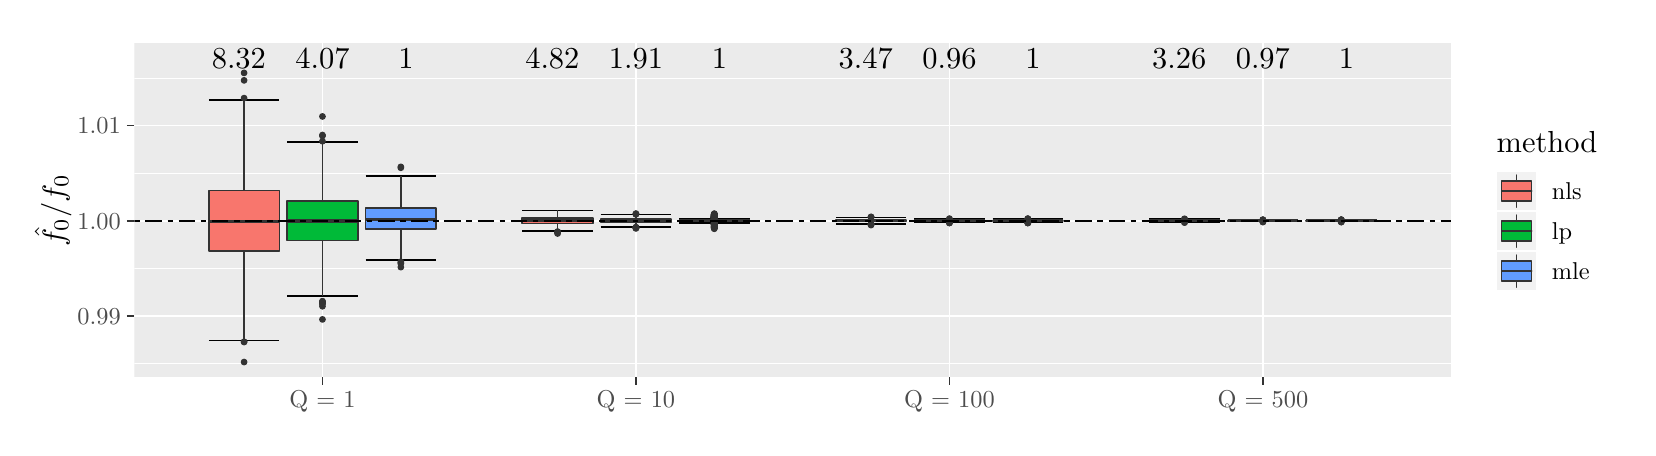
\begin{tikzpicture}[x=1pt,y=1pt]
\definecolor{fillColor}{RGB}{255,255,255}
\path[use as bounding box,fill=fillColor,fill opacity=0.00] (0,0) rectangle (578.16,144.54);
\begin{scope}
\path[clip] (  0.00,  0.00) rectangle (578.16,144.54);
\definecolor{drawColor}{RGB}{255,255,255}
\definecolor{fillColor}{RGB}{255,255,255}

\path[draw=drawColor,line width= 0.6pt,line join=round,line cap=round,fill=fillColor] (  0.00,  0.00) rectangle (578.16,144.54);
\end{scope}
\begin{scope}
\path[clip] ( 38.56, 18.22) rectangle (514.31,139.04);
\definecolor{fillColor}{gray}{0.92}

\path[fill=fillColor] ( 38.56, 18.22) rectangle (514.31,139.04);
\definecolor{drawColor}{RGB}{255,255,255}

\path[draw=drawColor,line width= 0.3pt,line join=round] ( 38.56, 23.12) --
	(514.31, 23.12);

\path[draw=drawColor,line width= 0.3pt,line join=round] ( 38.56, 57.54) --
	(514.31, 57.54);

\path[draw=drawColor,line width= 0.3pt,line join=round] ( 38.56, 91.95) --
	(514.31, 91.95);

\path[draw=drawColor,line width= 0.3pt,line join=round] ( 38.56,126.37) --
	(514.31,126.37);

\path[draw=drawColor,line width= 0.6pt,line join=round] ( 38.56, 40.33) --
	(514.31, 40.33);

\path[draw=drawColor,line width= 0.6pt,line join=round] ( 38.56, 74.75) --
	(514.31, 74.75);

\path[draw=drawColor,line width= 0.6pt,line join=round] ( 38.56,109.16) --
	(514.31,109.16);

\path[draw=drawColor,line width= 0.6pt,line join=round] (106.52, 18.22) --
	(106.52,139.04);

\path[draw=drawColor,line width= 0.6pt,line join=round] (219.79, 18.22) --
	(219.79,139.04);

\path[draw=drawColor,line width= 0.6pt,line join=round] (333.07, 18.22) --
	(333.07,139.04);

\path[draw=drawColor,line width= 0.6pt,line join=round] (446.34, 18.22) --
	(446.34,139.04);
\definecolor{drawColor}{RGB}{0,0,0}

\path[draw=drawColor,line width= 0.6pt,line join=round] ( 65.46,118.40) --
	( 90.94,118.40);

\path[draw=drawColor,line width= 0.6pt,line join=round] ( 78.20,118.40) --
	( 78.20, 31.50);

\path[draw=drawColor,line width= 0.6pt,line join=round] ( 65.46, 31.50) --
	( 90.94, 31.50);

\path[draw=drawColor,line width= 0.6pt,line join=round] ( 93.78,103.18) --
	(119.26,103.18);

\path[draw=drawColor,line width= 0.6pt,line join=round] (106.52,103.18) --
	(106.52, 47.51);

\path[draw=drawColor,line width= 0.6pt,line join=round] ( 93.78, 47.51) --
	(119.26, 47.51);

\path[draw=drawColor,line width= 0.6pt,line join=round] (122.09, 91.00) --
	(147.58, 91.00);

\path[draw=drawColor,line width= 0.6pt,line join=round] (134.84, 91.00) --
	(134.84, 60.48);

\path[draw=drawColor,line width= 0.6pt,line join=round] (122.09, 60.48) --
	(147.58, 60.48);

\path[draw=drawColor,line width= 0.6pt,line join=round] (178.73, 78.49) --
	(204.22, 78.49);

\path[draw=drawColor,line width= 0.6pt,line join=round] (191.48, 78.49) --
	(191.48, 71.04);

\path[draw=drawColor,line width= 0.6pt,line join=round] (178.73, 71.04) --
	(204.22, 71.04);

\path[draw=drawColor,line width= 0.6pt,line join=round] (207.05, 77.00) --
	(232.54, 77.00);

\path[draw=drawColor,line width= 0.6pt,line join=round] (219.79, 77.00) --
	(219.79, 72.45);

\path[draw=drawColor,line width= 0.6pt,line join=round] (207.05, 72.45) --
	(232.54, 72.45);

\path[draw=drawColor,line width= 0.6pt,line join=round] (235.37, 75.44) --
	(260.86, 75.44);

\path[draw=drawColor,line width= 0.6pt,line join=round] (248.11, 75.44) --
	(248.11, 74.01);

\path[draw=drawColor,line width= 0.6pt,line join=round] (235.37, 74.01) --
	(260.86, 74.01);

\path[draw=drawColor,line width= 0.6pt,line join=round] (292.01, 75.94) --
	(317.49, 75.94);

\path[draw=drawColor,line width= 0.6pt,line join=round] (304.75, 75.94) --
	(304.75, 73.55);

\path[draw=drawColor,line width= 0.6pt,line join=round] (292.01, 73.55) --
	(317.49, 73.55);

\path[draw=drawColor,line width= 0.6pt,line join=round] (320.33, 75.40) --
	(345.81, 75.40);

\path[draw=drawColor,line width= 0.6pt,line join=round] (333.07, 75.40) --
	(333.07, 74.10);

\path[draw=drawColor,line width= 0.6pt,line join=round] (320.33, 74.10) --
	(345.81, 74.10);

\path[draw=drawColor,line width= 0.6pt,line join=round] (348.64, 75.40) --
	(374.13, 75.40);

\path[draw=drawColor,line width= 0.6pt,line join=round] (361.39, 75.40) --
	(361.39, 74.11);

\path[draw=drawColor,line width= 0.6pt,line join=round] (348.64, 74.11) --
	(374.13, 74.11);

\path[draw=drawColor,line width= 0.6pt,line join=round] (405.28, 75.30) --
	(430.77, 75.30);

\path[draw=drawColor,line width= 0.6pt,line join=round] (418.02, 75.30) --
	(418.02, 74.22);

\path[draw=drawColor,line width= 0.6pt,line join=round] (405.28, 74.22) --
	(430.77, 74.22);

\path[draw=drawColor,line width= 0.6pt,line join=round] (433.60, 75.04) --
	(459.09, 75.04);

\path[draw=drawColor,line width= 0.6pt,line join=round] (446.34, 75.04) --
	(446.34, 74.45);

\path[draw=drawColor,line width= 0.6pt,line join=round] (433.60, 74.45) --
	(459.09, 74.45);

\path[draw=drawColor,line width= 0.6pt,line join=round] (461.92, 75.04) --
	(487.40, 75.04);

\path[draw=drawColor,line width= 0.6pt,line join=round] (474.66, 75.04) --
	(474.66, 74.46);

\path[draw=drawColor,line width= 0.6pt,line join=round] (461.92, 74.46) --
	(487.40, 74.46);
\definecolor{drawColor}{gray}{0.20}
\definecolor{fillColor}{gray}{0.20}

\path[draw=drawColor,line width= 0.4pt,line join=round,line cap=round,fill=fillColor] ( 78.20,119.08) circle (  1.02);

\path[draw=drawColor,line width= 0.4pt,line join=round,line cap=round,fill=fillColor] ( 78.20, 23.71) circle (  1.02);

\path[draw=drawColor,line width= 0.4pt,line join=round,line cap=round,fill=fillColor] ( 78.20, 30.97) circle (  1.02);

\path[draw=drawColor,line width= 0.4pt,line join=round,line cap=round,fill=fillColor] ( 78.20,125.50) circle (  1.02);

\path[draw=drawColor,line width= 0.4pt,line join=round,line cap=round,fill=fillColor] ( 78.20,128.20) circle (  1.02);

\path[draw=drawColor,line width= 0.4pt,line join=round,line cap=round,fill=fillColor] ( 78.20, 31.02) circle (  1.02);

\path[draw=drawColor,line width= 0.6pt,line join=round] ( 78.20, 85.75) -- ( 78.20,118.40);

\path[draw=drawColor,line width= 0.6pt,line join=round] ( 78.20, 63.90) -- ( 78.20, 31.50);
\definecolor{fillColor}{RGB}{248,118,109}

\path[draw=drawColor,line width= 0.6pt,line join=round,line cap=round,fill=fillColor] ( 65.46, 85.75) --
	( 65.46, 63.90) --
	( 90.94, 63.90) --
	( 90.94, 85.75) --
	( 65.46, 85.75) --
	cycle;

\path[draw=drawColor,line width= 1.1pt,line join=round] ( 65.46, 74.39) -- ( 90.94, 74.39);
\definecolor{fillColor}{gray}{0.20}

\path[draw=drawColor,line width= 0.4pt,line join=round,line cap=round,fill=fillColor] (106.52,105.41) circle (  1.02);

\path[draw=drawColor,line width= 0.4pt,line join=round,line cap=round,fill=fillColor] (106.52, 45.72) circle (  1.02);

\path[draw=drawColor,line width= 0.4pt,line join=round,line cap=round,fill=fillColor] (106.52,105.74) circle (  1.02);

\path[draw=drawColor,line width= 0.4pt,line join=round,line cap=round,fill=fillColor] (106.52,112.46) circle (  1.02);

\path[draw=drawColor,line width= 0.4pt,line join=round,line cap=round,fill=fillColor] (106.52, 45.26) circle (  1.02);

\path[draw=drawColor,line width= 0.4pt,line join=round,line cap=round,fill=fillColor] (106.52,103.51) circle (  1.02);

\path[draw=drawColor,line width= 0.4pt,line join=round,line cap=round,fill=fillColor] (106.52, 45.31) circle (  1.02);

\path[draw=drawColor,line width= 0.4pt,line join=round,line cap=round,fill=fillColor] (106.52, 39.12) circle (  1.02);

\path[draw=drawColor,line width= 0.4pt,line join=round,line cap=round,fill=fillColor] (106.52, 43.88) circle (  1.02);

\path[draw=drawColor,line width= 0.4pt,line join=round,line cap=round,fill=fillColor] (106.52, 45.02) circle (  1.02);

\path[draw=drawColor,line width= 0.4pt,line join=round,line cap=round,fill=fillColor] (106.52, 44.74) circle (  1.02);

\path[draw=drawColor,line width= 0.4pt,line join=round,line cap=round,fill=fillColor] (106.52, 45.22) circle (  1.02);

\path[draw=drawColor,line width= 0.6pt,line join=round] (106.52, 81.85) -- (106.52,103.18);

\path[draw=drawColor,line width= 0.6pt,line join=round] (106.52, 67.59) -- (106.52, 47.51);
\definecolor{fillColor}{RGB}{0,186,56}

\path[draw=drawColor,line width= 0.6pt,line join=round,line cap=round,fill=fillColor] ( 93.78, 81.85) --
	( 93.78, 67.59) --
	(119.26, 67.59) --
	(119.26, 81.85) --
	( 93.78, 81.85) --
	cycle;

\path[draw=drawColor,line width= 1.1pt,line join=round] ( 93.78, 74.68) -- (119.26, 74.68);
\definecolor{fillColor}{gray}{0.20}

\path[draw=drawColor,line width= 0.4pt,line join=round,line cap=round,fill=fillColor] (134.84, 93.92) circle (  1.02);

\path[draw=drawColor,line width= 0.4pt,line join=round,line cap=round,fill=fillColor] (134.84, 58.01) circle (  1.02);

\path[draw=drawColor,line width= 0.4pt,line join=round,line cap=round,fill=fillColor] (134.84, 59.34) circle (  1.02);

\path[draw=drawColor,line width= 0.4pt,line join=round,line cap=round,fill=fillColor] (134.84, 94.25) circle (  1.02);

\path[draw=drawColor,line width= 0.4pt,line join=round,line cap=round,fill=fillColor] (134.84, 59.54) circle (  1.02);

\path[draw=drawColor,line width= 0.4pt,line join=round,line cap=round,fill=fillColor] (134.84, 59.95) circle (  1.02);

\path[draw=drawColor,line width= 0.6pt,line join=round] (134.84, 79.45) -- (134.84, 91.00);

\path[draw=drawColor,line width= 0.6pt,line join=round] (134.84, 71.71) -- (134.84, 60.48);
\definecolor{fillColor}{RGB}{97,156,255}

\path[draw=drawColor,line width= 0.6pt,line join=round,line cap=round,fill=fillColor] (122.09, 79.45) --
	(122.09, 71.71) --
	(147.58, 71.71) --
	(147.58, 79.45) --
	(122.09, 79.45) --
	cycle;

\path[draw=drawColor,line width= 1.1pt,line join=round] (122.09, 75.39) -- (147.58, 75.39);
\definecolor{fillColor}{gray}{0.20}

\path[draw=drawColor,line width= 0.4pt,line join=round,line cap=round,fill=fillColor] (191.48, 70.81) circle (  1.02);

\path[draw=drawColor,line width= 0.4pt,line join=round,line cap=round,fill=fillColor] (191.48, 70.17) circle (  1.02);

\path[draw=drawColor,line width= 0.4pt,line join=round,line cap=round,fill=fillColor] (191.48, 70.48) circle (  1.02);

\path[draw=drawColor,line width= 0.4pt,line join=round,line cap=round,fill=fillColor] (191.48, 70.79) circle (  1.02);

\path[draw=drawColor,line width= 0.6pt,line join=round] (191.48, 75.68) -- (191.48, 78.49);

\path[draw=drawColor,line width= 0.6pt,line join=round] (191.48, 73.75) -- (191.48, 71.04);
\definecolor{fillColor}{RGB}{248,118,109}

\path[draw=drawColor,line width= 0.6pt,line join=round,line cap=round,fill=fillColor] (178.73, 75.68) --
	(178.73, 73.75) --
	(204.22, 73.75) --
	(204.22, 75.68) --
	(178.73, 75.68) --
	cycle;

\path[draw=drawColor,line width= 1.1pt,line join=round] (178.73, 74.72) -- (204.22, 74.72);
\definecolor{fillColor}{gray}{0.20}

\path[draw=drawColor,line width= 0.4pt,line join=round,line cap=round,fill=fillColor] (219.79, 77.36) circle (  1.02);

\path[draw=drawColor,line width= 0.4pt,line join=round,line cap=round,fill=fillColor] (219.79, 72.10) circle (  1.02);

\path[draw=drawColor,line width= 0.4pt,line join=round,line cap=round,fill=fillColor] (219.79, 72.33) circle (  1.02);

\path[draw=drawColor,line width= 0.4pt,line join=round,line cap=round,fill=fillColor] (219.79, 77.16) circle (  1.02);

\path[draw=drawColor,line width= 0.4pt,line join=round,line cap=round,fill=fillColor] (219.79, 72.30) circle (  1.02);

\path[draw=drawColor,line width= 0.4pt,line join=round,line cap=round,fill=fillColor] (219.79, 72.03) circle (  1.02);

\path[draw=drawColor,line width= 0.4pt,line join=round,line cap=round,fill=fillColor] (219.79, 77.12) circle (  1.02);

\path[draw=drawColor,line width= 0.4pt,line join=round,line cap=round,fill=fillColor] (219.79, 72.40) circle (  1.02);

\path[draw=drawColor,line width= 0.4pt,line join=round,line cap=round,fill=fillColor] (219.79, 72.31) circle (  1.02);

\path[draw=drawColor,line width= 0.4pt,line join=round,line cap=round,fill=fillColor] (219.79, 72.37) circle (  1.02);

\path[draw=drawColor,line width= 0.6pt,line join=round] (219.79, 75.33) -- (219.79, 77.00);

\path[draw=drawColor,line width= 0.6pt,line join=round] (219.79, 74.17) -- (219.79, 72.45);
\definecolor{fillColor}{RGB}{0,186,56}

\path[draw=drawColor,line width= 0.6pt,line join=round,line cap=round,fill=fillColor] (207.05, 75.33) --
	(207.05, 74.17) --
	(232.54, 74.17) --
	(232.54, 75.33) --
	(207.05, 75.33) --
	cycle;

\path[draw=drawColor,line width= 1.1pt,line join=round] (207.05, 74.75) -- (232.54, 74.75);
\definecolor{fillColor}{gray}{0.20}

\path[draw=drawColor,line width= 0.4pt,line join=round,line cap=round,fill=fillColor] (248.11, 76.17) circle (  1.02);

\path[draw=drawColor,line width= 0.4pt,line join=round,line cap=round,fill=fillColor] (248.11, 72.43) circle (  1.02);

\path[draw=drawColor,line width= 0.4pt,line join=round,line cap=round,fill=fillColor] (248.11, 76.15) circle (  1.02);

\path[draw=drawColor,line width= 0.4pt,line join=round,line cap=round,fill=fillColor] (248.11, 75.44) circle (  1.02);

\path[draw=drawColor,line width= 0.4pt,line join=round,line cap=round,fill=fillColor] (248.11, 73.54) circle (  1.02);

\path[draw=drawColor,line width= 0.4pt,line join=round,line cap=round,fill=fillColor] (248.11, 73.97) circle (  1.02);

\path[draw=drawColor,line width= 0.4pt,line join=round,line cap=round,fill=fillColor] (248.11, 73.81) circle (  1.02);

\path[draw=drawColor,line width= 0.4pt,line join=round,line cap=round,fill=fillColor] (248.11, 76.44) circle (  1.02);

\path[draw=drawColor,line width= 0.4pt,line join=round,line cap=round,fill=fillColor] (248.11, 73.67) circle (  1.02);

\path[draw=drawColor,line width= 0.4pt,line join=round,line cap=round,fill=fillColor] (248.11, 76.06) circle (  1.02);

\path[draw=drawColor,line width= 0.4pt,line join=round,line cap=round,fill=fillColor] (248.11, 75.87) circle (  1.02);

\path[draw=drawColor,line width= 0.4pt,line join=round,line cap=round,fill=fillColor] (248.11, 75.58) circle (  1.02);

\path[draw=drawColor,line width= 0.4pt,line join=round,line cap=round,fill=fillColor] (248.11, 76.05) circle (  1.02);

\path[draw=drawColor,line width= 0.4pt,line join=round,line cap=round,fill=fillColor] (248.11, 76.64) circle (  1.02);

\path[draw=drawColor,line width= 0.4pt,line join=round,line cap=round,fill=fillColor] (248.11, 75.46) circle (  1.02);

\path[draw=drawColor,line width= 0.4pt,line join=round,line cap=round,fill=fillColor] (248.11, 75.82) circle (  1.02);

\path[draw=drawColor,line width= 0.4pt,line join=round,line cap=round,fill=fillColor] (248.11, 75.83) circle (  1.02);

\path[draw=drawColor,line width= 0.4pt,line join=round,line cap=round,fill=fillColor] (248.11, 75.65) circle (  1.02);

\path[draw=drawColor,line width= 0.4pt,line join=round,line cap=round,fill=fillColor] (248.11, 75.81) circle (  1.02);

\path[draw=drawColor,line width= 0.4pt,line join=round,line cap=round,fill=fillColor] (248.11, 73.16) circle (  1.02);

\path[draw=drawColor,line width= 0.4pt,line join=round,line cap=round,fill=fillColor] (248.11, 77.22) circle (  1.02);

\path[draw=drawColor,line width= 0.4pt,line join=round,line cap=round,fill=fillColor] (248.11, 75.80) circle (  1.02);

\path[draw=drawColor,line width= 0.4pt,line join=round,line cap=round,fill=fillColor] (248.11, 73.97) circle (  1.02);

\path[draw=drawColor,line width= 0.4pt,line join=round,line cap=round,fill=fillColor] (248.11, 75.58) circle (  1.02);

\path[draw=drawColor,line width= 0.4pt,line join=round,line cap=round,fill=fillColor] (248.11, 75.85) circle (  1.02);

\path[draw=drawColor,line width= 0.4pt,line join=round,line cap=round,fill=fillColor] (248.11, 72.36) circle (  1.02);

\path[draw=drawColor,line width= 0.4pt,line join=round,line cap=round,fill=fillColor] (248.11, 76.42) circle (  1.02);

\path[draw=drawColor,line width= 0.4pt,line join=round,line cap=round,fill=fillColor] (248.11, 75.89) circle (  1.02);

\path[draw=drawColor,line width= 0.4pt,line join=round,line cap=round,fill=fillColor] (248.11, 76.03) circle (  1.02);

\path[draw=drawColor,line width= 0.4pt,line join=round,line cap=round,fill=fillColor] (248.11, 76.59) circle (  1.02);

\path[draw=drawColor,line width= 0.4pt,line join=round,line cap=round,fill=fillColor] (248.11, 75.99) circle (  1.02);

\path[draw=drawColor,line width= 0.4pt,line join=round,line cap=round,fill=fillColor] (248.11, 76.16) circle (  1.02);

\path[draw=drawColor,line width= 0.4pt,line join=round,line cap=round,fill=fillColor] (248.11, 76.20) circle (  1.02);

\path[draw=drawColor,line width= 0.4pt,line join=round,line cap=round,fill=fillColor] (248.11, 76.19) circle (  1.02);

\path[draw=drawColor,line width= 0.4pt,line join=round,line cap=round,fill=fillColor] (248.11, 75.46) circle (  1.02);

\path[draw=drawColor,line width= 0.4pt,line join=round,line cap=round,fill=fillColor] (248.11, 75.91) circle (  1.02);

\path[draw=drawColor,line width= 0.4pt,line join=round,line cap=round,fill=fillColor] (248.11, 75.73) circle (  1.02);

\path[draw=drawColor,line width= 0.4pt,line join=round,line cap=round,fill=fillColor] (248.11, 75.92) circle (  1.02);

\path[draw=drawColor,line width= 0.4pt,line join=round,line cap=round,fill=fillColor] (248.11, 75.45) circle (  1.02);

\path[draw=drawColor,line width= 0.4pt,line join=round,line cap=round,fill=fillColor] (248.11, 76.15) circle (  1.02);

\path[draw=drawColor,line width= 0.4pt,line join=round,line cap=round,fill=fillColor] (248.11, 72.57) circle (  1.02);

\path[draw=drawColor,line width= 0.4pt,line join=round,line cap=round,fill=fillColor] (248.11, 71.99) circle (  1.02);

\path[draw=drawColor,line width= 0.4pt,line join=round,line cap=round,fill=fillColor] (248.11, 73.78) circle (  1.02);

\path[draw=drawColor,line width= 0.4pt,line join=round,line cap=round,fill=fillColor] (248.11, 76.22) circle (  1.02);

\path[draw=drawColor,line width= 0.4pt,line join=round,line cap=round,fill=fillColor] (248.11, 75.75) circle (  1.02);

\path[draw=drawColor,line width= 0.4pt,line join=round,line cap=round,fill=fillColor] (248.11, 76.20) circle (  1.02);

\path[draw=drawColor,line width= 0.4pt,line join=round,line cap=round,fill=fillColor] (248.11, 76.21) circle (  1.02);

\path[draw=drawColor,line width= 0.4pt,line join=round,line cap=round,fill=fillColor] (248.11, 75.72) circle (  1.02);

\path[draw=drawColor,line width= 0.4pt,line join=round,line cap=round,fill=fillColor] (248.11, 76.14) circle (  1.02);

\path[draw=drawColor,line width= 0.4pt,line join=round,line cap=round,fill=fillColor] (248.11, 75.74) circle (  1.02);

\path[draw=drawColor,line width= 0.4pt,line join=round,line cap=round,fill=fillColor] (248.11, 75.58) circle (  1.02);

\path[draw=drawColor,line width= 0.4pt,line join=round,line cap=round,fill=fillColor] (248.11, 76.13) circle (  1.02);

\path[draw=drawColor,line width= 0.4pt,line join=round,line cap=round,fill=fillColor] (248.11, 76.97) circle (  1.02);

\path[draw=drawColor,line width= 0.4pt,line join=round,line cap=round,fill=fillColor] (248.11, 73.63) circle (  1.02);

\path[draw=drawColor,line width= 0.4pt,line join=round,line cap=round,fill=fillColor] (248.11, 76.95) circle (  1.02);

\path[draw=drawColor,line width= 0.4pt,line join=round,line cap=round,fill=fillColor] (248.11, 75.71) circle (  1.02);

\path[draw=drawColor,line width= 0.4pt,line join=round,line cap=round,fill=fillColor] (248.11, 76.95) circle (  1.02);

\path[draw=drawColor,line width= 0.4pt,line join=round,line cap=round,fill=fillColor] (248.11, 75.47) circle (  1.02);

\path[draw=drawColor,line width= 0.4pt,line join=round,line cap=round,fill=fillColor] (248.11, 75.82) circle (  1.02);

\path[draw=drawColor,line width= 0.4pt,line join=round,line cap=round,fill=fillColor] (248.11, 75.50) circle (  1.02);

\path[draw=drawColor,line width= 0.4pt,line join=round,line cap=round,fill=fillColor] (248.11, 76.33) circle (  1.02);

\path[draw=drawColor,line width= 0.4pt,line join=round,line cap=round,fill=fillColor] (248.11, 73.94) circle (  1.02);

\path[draw=drawColor,line width= 0.4pt,line join=round,line cap=round,fill=fillColor] (248.11, 75.76) circle (  1.02);

\path[draw=drawColor,line width= 0.4pt,line join=round,line cap=round,fill=fillColor] (248.11, 73.54) circle (  1.02);

\path[draw=drawColor,line width= 0.4pt,line join=round,line cap=round,fill=fillColor] (248.11, 73.61) circle (  1.02);

\path[draw=drawColor,line width= 0.4pt,line join=round,line cap=round,fill=fillColor] (248.11, 73.10) circle (  1.02);

\path[draw=drawColor,line width= 0.4pt,line join=round,line cap=round,fill=fillColor] (248.11, 76.98) circle (  1.02);

\path[draw=drawColor,line width= 0.4pt,line join=round,line cap=round,fill=fillColor] (248.11, 75.94) circle (  1.02);

\path[draw=drawColor,line width= 0.4pt,line join=round,line cap=round,fill=fillColor] (248.11, 76.10) circle (  1.02);

\path[draw=drawColor,line width= 0.4pt,line join=round,line cap=round,fill=fillColor] (248.11, 73.88) circle (  1.02);

\path[draw=drawColor,line width= 0.4pt,line join=round,line cap=round,fill=fillColor] (248.11, 76.44) circle (  1.02);

\path[draw=drawColor,line width= 0.4pt,line join=round,line cap=round,fill=fillColor] (248.11, 75.59) circle (  1.02);

\path[draw=drawColor,line width= 0.4pt,line join=round,line cap=round,fill=fillColor] (248.11, 76.35) circle (  1.02);

\path[draw=drawColor,line width= 0.4pt,line join=round,line cap=round,fill=fillColor] (248.11, 73.91) circle (  1.02);

\path[draw=drawColor,line width= 0.4pt,line join=round,line cap=round,fill=fillColor] (248.11, 72.87) circle (  1.02);

\path[draw=drawColor,line width= 0.4pt,line join=round,line cap=round,fill=fillColor] (248.11, 76.77) circle (  1.02);

\path[draw=drawColor,line width= 0.4pt,line join=round,line cap=round,fill=fillColor] (248.11, 77.02) circle (  1.02);

\path[draw=drawColor,line width= 0.4pt,line join=round,line cap=round,fill=fillColor] (248.11, 75.48) circle (  1.02);

\path[draw=drawColor,line width= 0.4pt,line join=round,line cap=round,fill=fillColor] (248.11, 76.66) circle (  1.02);

\path[draw=drawColor,line width= 0.4pt,line join=round,line cap=round,fill=fillColor] (248.11, 75.69) circle (  1.02);

\path[draw=drawColor,line width= 0.4pt,line join=round,line cap=round,fill=fillColor] (248.11, 76.75) circle (  1.02);

\path[draw=drawColor,line width= 0.4pt,line join=round,line cap=round,fill=fillColor] (248.11, 72.43) circle (  1.02);

\path[draw=drawColor,line width= 0.4pt,line join=round,line cap=round,fill=fillColor] (248.11, 75.73) circle (  1.02);

\path[draw=drawColor,line width= 0.4pt,line join=round,line cap=round,fill=fillColor] (248.11, 75.63) circle (  1.02);

\path[draw=drawColor,line width= 0.4pt,line join=round,line cap=round,fill=fillColor] (248.11, 75.45) circle (  1.02);

\path[draw=drawColor,line width= 0.4pt,line join=round,line cap=round,fill=fillColor] (248.11, 73.53) circle (  1.02);

\path[draw=drawColor,line width= 0.4pt,line join=round,line cap=round,fill=fillColor] (248.11, 75.90) circle (  1.02);

\path[draw=drawColor,line width= 0.4pt,line join=round,line cap=round,fill=fillColor] (248.11, 76.14) circle (  1.02);

\path[draw=drawColor,line width= 0.4pt,line join=round,line cap=round,fill=fillColor] (248.11, 77.33) circle (  1.02);

\path[draw=drawColor,line width= 0.4pt,line join=round,line cap=round,fill=fillColor] (248.11, 77.11) circle (  1.02);

\path[draw=drawColor,line width= 0.4pt,line join=round,line cap=round,fill=fillColor] (248.11, 75.74) circle (  1.02);

\path[draw=drawColor,line width= 0.4pt,line join=round,line cap=round,fill=fillColor] (248.11, 75.92) circle (  1.02);

\path[draw=drawColor,line width= 0.4pt,line join=round,line cap=round,fill=fillColor] (248.11, 76.46) circle (  1.02);

\path[draw=drawColor,line width= 0.4pt,line join=round,line cap=round,fill=fillColor] (248.11, 76.18) circle (  1.02);

\path[draw=drawColor,line width= 0.4pt,line join=round,line cap=round,fill=fillColor] (248.11, 73.44) circle (  1.02);

\path[draw=drawColor,line width= 0.4pt,line join=round,line cap=round,fill=fillColor] (248.11, 75.83) circle (  1.02);

\path[draw=drawColor,line width= 0.4pt,line join=round,line cap=round,fill=fillColor] (248.11, 73.63) circle (  1.02);

\path[draw=drawColor,line width= 0.4pt,line join=round,line cap=round,fill=fillColor] (248.11, 76.12) circle (  1.02);

\path[draw=drawColor,line width= 0.4pt,line join=round,line cap=round,fill=fillColor] (248.11, 75.85) circle (  1.02);

\path[draw=drawColor,line width= 0.4pt,line join=round,line cap=round,fill=fillColor] (248.11, 75.63) circle (  1.02);

\path[draw=drawColor,line width= 0.4pt,line join=round,line cap=round,fill=fillColor] (248.11, 76.43) circle (  1.02);

\path[draw=drawColor,line width= 0.4pt,line join=round,line cap=round,fill=fillColor] (248.11, 71.90) circle (  1.02);

\path[draw=drawColor,line width= 0.4pt,line join=round,line cap=round,fill=fillColor] (248.11, 73.30) circle (  1.02);

\path[draw=drawColor,line width= 0.4pt,line join=round,line cap=round,fill=fillColor] (248.11, 75.71) circle (  1.02);

\path[draw=drawColor,line width= 0.4pt,line join=round,line cap=round,fill=fillColor] (248.11, 76.20) circle (  1.02);

\path[draw=drawColor,line width= 0.4pt,line join=round,line cap=round,fill=fillColor] (248.11, 73.26) circle (  1.02);

\path[draw=drawColor,line width= 0.4pt,line join=round,line cap=round,fill=fillColor] (248.11, 73.39) circle (  1.02);

\path[draw=drawColor,line width= 0.4pt,line join=round,line cap=round,fill=fillColor] (248.11, 75.94) circle (  1.02);

\path[draw=drawColor,line width= 0.4pt,line join=round,line cap=round,fill=fillColor] (248.11, 76.23) circle (  1.02);

\path[draw=drawColor,line width= 0.4pt,line join=round,line cap=round,fill=fillColor] (248.11, 75.45) circle (  1.02);

\path[draw=drawColor,line width= 0.4pt,line join=round,line cap=round,fill=fillColor] (248.11, 76.22) circle (  1.02);

\path[draw=drawColor,line width= 0.4pt,line join=round,line cap=round,fill=fillColor] (248.11, 72.80) circle (  1.02);

\path[draw=drawColor,line width= 0.4pt,line join=round,line cap=round,fill=fillColor] (248.11, 73.84) circle (  1.02);

\path[draw=drawColor,line width= 0.4pt,line join=round,line cap=round,fill=fillColor] (248.11, 72.45) circle (  1.02);

\path[draw=drawColor,line width= 0.4pt,line join=round,line cap=round,fill=fillColor] (248.11, 75.62) circle (  1.02);

\path[draw=drawColor,line width= 0.4pt,line join=round,line cap=round,fill=fillColor] (248.11, 76.07) circle (  1.02);

\path[draw=drawColor,line width= 0.4pt,line join=round,line cap=round,fill=fillColor] (248.11, 76.62) circle (  1.02);

\path[draw=drawColor,line width= 0.4pt,line join=round,line cap=round,fill=fillColor] (248.11, 76.22) circle (  1.02);

\path[draw=drawColor,line width= 0.4pt,line join=round,line cap=round,fill=fillColor] (248.11, 72.95) circle (  1.02);

\path[draw=drawColor,line width= 0.4pt,line join=round,line cap=round,fill=fillColor] (248.11, 75.63) circle (  1.02);

\path[draw=drawColor,line width= 0.4pt,line join=round,line cap=round,fill=fillColor] (248.11, 73.96) circle (  1.02);

\path[draw=drawColor,line width= 0.4pt,line join=round,line cap=round,fill=fillColor] (248.11, 75.65) circle (  1.02);

\path[draw=drawColor,line width= 0.4pt,line join=round,line cap=round,fill=fillColor] (248.11, 75.99) circle (  1.02);

\path[draw=drawColor,line width= 0.4pt,line join=round,line cap=round,fill=fillColor] (248.11, 76.96) circle (  1.02);

\path[draw=drawColor,line width= 0.4pt,line join=round,line cap=round,fill=fillColor] (248.11, 75.48) circle (  1.02);

\path[draw=drawColor,line width= 0.4pt,line join=round,line cap=round,fill=fillColor] (248.11, 76.19) circle (  1.02);

\path[draw=drawColor,line width= 0.4pt,line join=round,line cap=round,fill=fillColor] (248.11, 75.91) circle (  1.02);

\path[draw=drawColor,line width= 0.4pt,line join=round,line cap=round,fill=fillColor] (248.11, 73.30) circle (  1.02);

\path[draw=drawColor,line width= 0.4pt,line join=round,line cap=round,fill=fillColor] (248.11, 72.71) circle (  1.02);

\path[draw=drawColor,line width= 0.4pt,line join=round,line cap=round,fill=fillColor] (248.11, 73.34) circle (  1.02);

\path[draw=drawColor,line width= 0.4pt,line join=round,line cap=round,fill=fillColor] (248.11, 76.46) circle (  1.02);

\path[draw=drawColor,line width= 0.4pt,line join=round,line cap=round,fill=fillColor] (248.11, 73.93) circle (  1.02);

\path[draw=drawColor,line width= 0.4pt,line join=round,line cap=round,fill=fillColor] (248.11, 72.50) circle (  1.02);

\path[draw=drawColor,line width= 0.4pt,line join=round,line cap=round,fill=fillColor] (248.11, 76.03) circle (  1.02);

\path[draw=drawColor,line width= 0.4pt,line join=round,line cap=round,fill=fillColor] (248.11, 75.89) circle (  1.02);

\path[draw=drawColor,line width= 0.4pt,line join=round,line cap=round,fill=fillColor] (248.11, 76.03) circle (  1.02);

\path[draw=drawColor,line width= 0.4pt,line join=round,line cap=round,fill=fillColor] (248.11, 76.41) circle (  1.02);

\path[draw=drawColor,line width= 0.4pt,line join=round,line cap=round,fill=fillColor] (248.11, 76.06) circle (  1.02);

\path[draw=drawColor,line width= 0.4pt,line join=round,line cap=round,fill=fillColor] (248.11, 72.25) circle (  1.02);

\path[draw=drawColor,line width= 0.4pt,line join=round,line cap=round,fill=fillColor] (248.11, 75.78) circle (  1.02);

\path[draw=drawColor,line width= 0.4pt,line join=round,line cap=round,fill=fillColor] (248.11, 76.66) circle (  1.02);

\path[draw=drawColor,line width= 0.4pt,line join=round,line cap=round,fill=fillColor] (248.11, 73.68) circle (  1.02);

\path[draw=drawColor,line width= 0.4pt,line join=round,line cap=round,fill=fillColor] (248.11, 75.46) circle (  1.02);

\path[draw=drawColor,line width= 0.4pt,line join=round,line cap=round,fill=fillColor] (248.11, 73.97) circle (  1.02);

\path[draw=drawColor,line width= 0.4pt,line join=round,line cap=round,fill=fillColor] (248.11, 76.13) circle (  1.02);

\path[draw=drawColor,line width= 0.4pt,line join=round,line cap=round,fill=fillColor] (248.11, 75.74) circle (  1.02);

\path[draw=drawColor,line width= 0.4pt,line join=round,line cap=round,fill=fillColor] (248.11, 73.50) circle (  1.02);

\path[draw=drawColor,line width= 0.4pt,line join=round,line cap=round,fill=fillColor] (248.11, 72.68) circle (  1.02);

\path[draw=drawColor,line width= 0.4pt,line join=round,line cap=round,fill=fillColor] (248.11, 73.47) circle (  1.02);

\path[draw=drawColor,line width= 0.4pt,line join=round,line cap=round,fill=fillColor] (248.11, 76.66) circle (  1.02);

\path[draw=drawColor,line width= 0.4pt,line join=round,line cap=round,fill=fillColor] (248.11, 75.87) circle (  1.02);

\path[draw=drawColor,line width= 0.4pt,line join=round,line cap=round,fill=fillColor] (248.11, 73.49) circle (  1.02);

\path[draw=drawColor,line width= 0.4pt,line join=round,line cap=round,fill=fillColor] (248.11, 75.67) circle (  1.02);

\path[draw=drawColor,line width= 0.4pt,line join=round,line cap=round,fill=fillColor] (248.11, 76.72) circle (  1.02);

\path[draw=drawColor,line width= 0.4pt,line join=round,line cap=round,fill=fillColor] (248.11, 76.02) circle (  1.02);

\path[draw=drawColor,line width= 0.4pt,line join=round,line cap=round,fill=fillColor] (248.11, 76.01) circle (  1.02);

\path[draw=drawColor,line width= 0.4pt,line join=round,line cap=round,fill=fillColor] (248.11, 76.76) circle (  1.02);

\path[draw=drawColor,line width= 0.4pt,line join=round,line cap=round,fill=fillColor] (248.11, 76.45) circle (  1.02);

\path[draw=drawColor,line width= 0.4pt,line join=round,line cap=round,fill=fillColor] (248.11, 75.63) circle (  1.02);

\path[draw=drawColor,line width= 0.4pt,line join=round,line cap=round,fill=fillColor] (248.11, 75.89) circle (  1.02);

\path[draw=drawColor,line width= 0.4pt,line join=round,line cap=round,fill=fillColor] (248.11, 75.88) circle (  1.02);

\path[draw=drawColor,line width= 0.4pt,line join=round,line cap=round,fill=fillColor] (248.11, 75.81) circle (  1.02);

\path[draw=drawColor,line width= 0.6pt,line join=round] (248.11, 74.89) -- (248.11, 75.44);

\path[draw=drawColor,line width= 0.6pt,line join=round] (248.11, 74.53) -- (248.11, 74.01);
\definecolor{fillColor}{RGB}{97,156,255}

\path[draw=drawColor,line width= 0.6pt,line join=round,line cap=round,fill=fillColor] (235.37, 74.89) --
	(235.37, 74.53) --
	(260.86, 74.53) --
	(260.86, 74.89) --
	(235.37, 74.89) --
	cycle;

\path[draw=drawColor,line width= 1.1pt,line join=round] (235.37, 74.70) -- (260.86, 74.70);
\definecolor{fillColor}{gray}{0.20}

\path[draw=drawColor,line width= 0.4pt,line join=round,line cap=round,fill=fillColor] (304.75, 76.17) circle (  1.02);

\path[draw=drawColor,line width= 0.4pt,line join=round,line cap=round,fill=fillColor] (304.75, 73.20) circle (  1.02);

\path[draw=drawColor,line width= 0.4pt,line join=round,line cap=round,fill=fillColor] (304.75, 76.05) circle (  1.02);

\path[draw=drawColor,line width= 0.4pt,line join=round,line cap=round,fill=fillColor] (304.75, 73.52) circle (  1.02);

\path[draw=drawColor,line width= 0.4pt,line join=round,line cap=round,fill=fillColor] (304.75, 73.51) circle (  1.02);

\path[draw=drawColor,line width= 0.4pt,line join=round,line cap=round,fill=fillColor] (304.75, 73.47) circle (  1.02);

\path[draw=drawColor,line width= 0.4pt,line join=round,line cap=round,fill=fillColor] (304.75, 76.05) circle (  1.02);

\path[draw=drawColor,line width= 0.4pt,line join=round,line cap=round,fill=fillColor] (304.75, 73.53) circle (  1.02);

\path[draw=drawColor,line width= 0.6pt,line join=round] (304.75, 75.06) -- (304.75, 75.94);

\path[draw=drawColor,line width= 0.6pt,line join=round] (304.75, 74.45) -- (304.75, 73.55);
\definecolor{fillColor}{RGB}{248,118,109}

\path[draw=drawColor,line width= 0.6pt,line join=round,line cap=round,fill=fillColor] (292.01, 75.06) --
	(292.01, 74.45) --
	(317.49, 74.45) --
	(317.49, 75.06) --
	(292.01, 75.06) --
	cycle;

\path[draw=drawColor,line width= 1.1pt,line join=round] (292.01, 74.75) -- (317.49, 74.75);
\definecolor{fillColor}{gray}{0.20}

\path[draw=drawColor,line width= 0.4pt,line join=round,line cap=round,fill=fillColor] (333.07, 74.06) circle (  1.02);

\path[draw=drawColor,line width= 0.4pt,line join=round,line cap=round,fill=fillColor] (333.07, 75.53) circle (  1.02);

\path[draw=drawColor,line width= 0.4pt,line join=round,line cap=round,fill=fillColor] (333.07, 75.41) circle (  1.02);

\path[draw=drawColor,line width= 0.4pt,line join=round,line cap=round,fill=fillColor] (333.07, 74.03) circle (  1.02);

\path[draw=drawColor,line width= 0.4pt,line join=round,line cap=round,fill=fillColor] (333.07, 73.96) circle (  1.02);

\path[draw=drawColor,line width= 0.6pt,line join=round] (333.07, 74.91) -- (333.07, 75.40);

\path[draw=drawColor,line width= 0.6pt,line join=round] (333.07, 74.59) -- (333.07, 74.10);
\definecolor{fillColor}{RGB}{0,186,56}

\path[draw=drawColor,line width= 0.6pt,line join=round,line cap=round,fill=fillColor] (320.33, 74.91) --
	(320.33, 74.59) --
	(345.81, 74.59) --
	(345.81, 74.91) --
	(320.33, 74.91) --
	cycle;

\path[draw=drawColor,line width= 1.1pt,line join=round] (320.33, 74.74) -- (345.81, 74.74);
\definecolor{fillColor}{gray}{0.20}

\path[draw=drawColor,line width= 0.4pt,line join=round,line cap=round,fill=fillColor] (361.39, 74.05) circle (  1.02);

\path[draw=drawColor,line width= 0.4pt,line join=round,line cap=round,fill=fillColor] (361.39, 75.51) circle (  1.02);

\path[draw=drawColor,line width= 0.4pt,line join=round,line cap=round,fill=fillColor] (361.39, 75.49) circle (  1.02);

\path[draw=drawColor,line width= 0.4pt,line join=round,line cap=round,fill=fillColor] (361.39, 75.42) circle (  1.02);

\path[draw=drawColor,line width= 0.4pt,line join=round,line cap=round,fill=fillColor] (361.39, 74.07) circle (  1.02);

\path[draw=drawColor,line width= 0.4pt,line join=round,line cap=round,fill=fillColor] (361.39, 74.00) circle (  1.02);

\path[draw=drawColor,line width= 0.4pt,line join=round,line cap=round,fill=fillColor] (361.39, 74.02) circle (  1.02);

\path[draw=drawColor,line width= 0.4pt,line join=round,line cap=round,fill=fillColor] (361.39, 73.97) circle (  1.02);

\path[draw=drawColor,line width= 0.6pt,line join=round] (361.39, 74.91) -- (361.39, 75.40);

\path[draw=drawColor,line width= 0.6pt,line join=round] (361.39, 74.58) -- (361.39, 74.11);
\definecolor{fillColor}{RGB}{97,156,255}

\path[draw=drawColor,line width= 0.6pt,line join=round,line cap=round,fill=fillColor] (348.64, 74.91) --
	(348.64, 74.58) --
	(374.13, 74.58) --
	(374.13, 74.91) --
	(348.64, 74.91) --
	cycle;

\path[draw=drawColor,line width= 1.1pt,line join=round] (348.64, 74.74) -- (374.13, 74.74);
\definecolor{fillColor}{gray}{0.20}

\path[draw=drawColor,line width= 0.4pt,line join=round,line cap=round,fill=fillColor] (418.02, 75.37) circle (  1.02);

\path[draw=drawColor,line width= 0.4pt,line join=round,line cap=round,fill=fillColor] (418.02, 75.45) circle (  1.02);

\path[draw=drawColor,line width= 0.4pt,line join=round,line cap=round,fill=fillColor] (418.02, 75.36) circle (  1.02);

\path[draw=drawColor,line width= 0.4pt,line join=round,line cap=round,fill=fillColor] (418.02, 74.14) circle (  1.02);

\path[draw=drawColor,line width= 0.4pt,line join=round,line cap=round,fill=fillColor] (418.02, 74.13) circle (  1.02);

\path[draw=drawColor,line width= 0.6pt,line join=round] (418.02, 74.88) -- (418.02, 75.30);

\path[draw=drawColor,line width= 0.6pt,line join=round] (418.02, 74.60) -- (418.02, 74.22);
\definecolor{fillColor}{RGB}{248,118,109}

\path[draw=drawColor,line width= 0.6pt,line join=round,line cap=round,fill=fillColor] (405.28, 74.88) --
	(405.28, 74.60) --
	(430.77, 74.60) --
	(430.77, 74.88) --
	(405.28, 74.88) --
	cycle;

\path[draw=drawColor,line width= 1.1pt,line join=round] (405.28, 74.73) -- (430.77, 74.73);
\definecolor{fillColor}{gray}{0.20}

\path[draw=drawColor,line width= 0.4pt,line join=round,line cap=round,fill=fillColor] (446.34, 75.12) circle (  1.02);

\path[draw=drawColor,line width= 0.4pt,line join=round,line cap=round,fill=fillColor] (446.34, 75.06) circle (  1.02);

\path[draw=drawColor,line width= 0.4pt,line join=round,line cap=round,fill=fillColor] (446.34, 74.37) circle (  1.02);

\path[draw=drawColor,line width= 0.4pt,line join=round,line cap=round,fill=fillColor] (446.34, 75.09) circle (  1.02);

\path[draw=drawColor,line width= 0.4pt,line join=round,line cap=round,fill=fillColor] (446.34, 75.09) circle (  1.02);

\path[draw=drawColor,line width= 0.4pt,line join=round,line cap=round,fill=fillColor] (446.34, 74.33) circle (  1.02);

\path[draw=drawColor,line width= 0.4pt,line join=round,line cap=round,fill=fillColor] (446.34, 74.38) circle (  1.02);

\path[draw=drawColor,line width= 0.6pt,line join=round] (446.34, 74.82) -- (446.34, 75.04);

\path[draw=drawColor,line width= 0.6pt,line join=round] (446.34, 74.67) -- (446.34, 74.45);
\definecolor{fillColor}{RGB}{0,186,56}

\path[draw=drawColor,line width= 0.6pt,line join=round,line cap=round,fill=fillColor] (433.60, 74.82) --
	(433.60, 74.67) --
	(459.09, 74.67) --
	(459.09, 74.82) --
	(433.60, 74.82) --
	cycle;

\path[draw=drawColor,line width= 1.1pt,line join=round] (433.60, 74.74) -- (459.09, 74.74);
\definecolor{fillColor}{gray}{0.20}

\path[draw=drawColor,line width= 0.4pt,line join=round,line cap=round,fill=fillColor] (474.66, 75.14) circle (  1.02);

\path[draw=drawColor,line width= 0.4pt,line join=round,line cap=round,fill=fillColor] (474.66, 75.07) circle (  1.02);

\path[draw=drawColor,line width= 0.4pt,line join=round,line cap=round,fill=fillColor] (474.66, 74.32) circle (  1.02);

\path[draw=drawColor,line width= 0.4pt,line join=round,line cap=round,fill=fillColor] (474.66, 75.11) circle (  1.02);

\path[draw=drawColor,line width= 0.4pt,line join=round,line cap=round,fill=fillColor] (474.66, 75.08) circle (  1.02);

\path[draw=drawColor,line width= 0.4pt,line join=round,line cap=round,fill=fillColor] (474.66, 74.32) circle (  1.02);

\path[draw=drawColor,line width= 0.4pt,line join=round,line cap=round,fill=fillColor] (474.66, 74.43) circle (  1.02);

\path[draw=drawColor,line width= 0.4pt,line join=round,line cap=round,fill=fillColor] (474.66, 74.43) circle (  1.02);

\path[draw=drawColor,line width= 0.4pt,line join=round,line cap=round,fill=fillColor] (474.66, 75.07) circle (  1.02);

\path[draw=drawColor,line width= 0.6pt,line join=round] (474.66, 74.83) -- (474.66, 75.04);

\path[draw=drawColor,line width= 0.6pt,line join=round] (474.66, 74.68) -- (474.66, 74.46);
\definecolor{fillColor}{RGB}{97,156,255}

\path[draw=drawColor,line width= 0.6pt,line join=round,line cap=round,fill=fillColor] (461.92, 74.83) --
	(461.92, 74.68) --
	(487.40, 74.68) --
	(487.40, 74.83) --
	(461.92, 74.83) --
	cycle;

\path[draw=drawColor,line width= 1.1pt,line join=round] (461.92, 74.75) -- (487.40, 74.75);
\definecolor{drawColor}{RGB}{0,0,0}

\path[draw=drawColor,line width= 0.6pt,dash pattern=on 2pt off 2pt on 6pt off 2pt ,line join=round] ( 38.56, 74.75) -- (514.31, 74.75);

\node[text=drawColor,anchor=base,inner sep=0pt, outer sep=0pt, scale=  1.10] at (136.73,129.75) {1};

\node[text=drawColor,anchor=base,inner sep=0pt, outer sep=0pt, scale=  1.10] at (106.52,129.75) {4.07};

\node[text=drawColor,anchor=base,inner sep=0pt, outer sep=0pt, scale=  1.10] at ( 76.31,129.75) {8.32};

\node[text=drawColor,anchor=base,inner sep=0pt, outer sep=0pt, scale=  1.10] at (250.00,129.75) {1};

\node[text=drawColor,anchor=base,inner sep=0pt, outer sep=0pt, scale=  1.10] at (219.79,129.75) {1.91};

\node[text=drawColor,anchor=base,inner sep=0pt, outer sep=0pt, scale=  1.10] at (189.59,129.75) {4.82};

\node[text=drawColor,anchor=base,inner sep=0pt, outer sep=0pt, scale=  1.10] at (363.28,129.75) {1};

\node[text=drawColor,anchor=base,inner sep=0pt, outer sep=0pt, scale=  1.10] at (333.07,129.75) {0.96};

\node[text=drawColor,anchor=base,inner sep=0pt, outer sep=0pt, scale=  1.10] at (302.86,129.75) {3.47};

\node[text=drawColor,anchor=base,inner sep=0pt, outer sep=0pt, scale=  1.10] at (476.55,129.75) {1};

\node[text=drawColor,anchor=base,inner sep=0pt, outer sep=0pt, scale=  1.10] at (446.34,129.75) {0.97};

\node[text=drawColor,anchor=base,inner sep=0pt, outer sep=0pt, scale=  1.10] at (416.14,129.75) {3.26};
\end{scope}
\begin{scope}
\path[clip] (  0.00,  0.00) rectangle (578.16,144.54);
\definecolor{drawColor}{gray}{0.30}

\node[text=drawColor,anchor=base east,inner sep=0pt, outer sep=0pt, scale=  0.88] at ( 33.61, 37.30) {0.99};

\node[text=drawColor,anchor=base east,inner sep=0pt, outer sep=0pt, scale=  0.88] at ( 33.61, 71.71) {1.00};

\node[text=drawColor,anchor=base east,inner sep=0pt, outer sep=0pt, scale=  0.88] at ( 33.61,106.13) {1.01};
\end{scope}
\begin{scope}
\path[clip] (  0.00,  0.00) rectangle (578.16,144.54);
\definecolor{drawColor}{gray}{0.20}

\path[draw=drawColor,line width= 0.6pt,line join=round] ( 35.81, 40.33) --
	( 38.56, 40.33);

\path[draw=drawColor,line width= 0.6pt,line join=round] ( 35.81, 74.75) --
	( 38.56, 74.75);

\path[draw=drawColor,line width= 0.6pt,line join=round] ( 35.81,109.16) --
	( 38.56,109.16);
\end{scope}
\begin{scope}
\path[clip] (  0.00,  0.00) rectangle (578.16,144.54);
\definecolor{drawColor}{gray}{0.20}

\path[draw=drawColor,line width= 0.6pt,line join=round] (106.52, 15.47) --
	(106.52, 18.22);

\path[draw=drawColor,line width= 0.6pt,line join=round] (219.79, 15.47) --
	(219.79, 18.22);

\path[draw=drawColor,line width= 0.6pt,line join=round] (333.07, 15.47) --
	(333.07, 18.22);

\path[draw=drawColor,line width= 0.6pt,line join=round] (446.34, 15.47) --
	(446.34, 18.22);
\end{scope}
\begin{scope}
\path[clip] (  0.00,  0.00) rectangle (578.16,144.54);
\definecolor{drawColor}{gray}{0.30}

\node[text=drawColor,anchor=base,inner sep=0pt, outer sep=0pt, scale=  0.88] at (106.52,  7.21) {Q = 1};

\node[text=drawColor,anchor=base,inner sep=0pt, outer sep=0pt, scale=  0.88] at (219.79,  7.21) {Q = 10};

\node[text=drawColor,anchor=base,inner sep=0pt, outer sep=0pt, scale=  0.88] at (333.07,  7.21) {Q = 100};

\node[text=drawColor,anchor=base,inner sep=0pt, outer sep=0pt, scale=  0.88] at (446.34,  7.21) {Q = 500};
\end{scope}
\begin{scope}
\path[clip] (  0.00,  0.00) rectangle (578.16,144.54);
\definecolor{drawColor}{RGB}{0,0,0}

\node[text=drawColor,rotate= 90.00,anchor=base,inner sep=0pt, outer sep=0pt, scale=  1.10] at ( 13.08, 78.63) {$\hat{f_0}/f_0$};
\end{scope}
\begin{scope}
\path[clip] (  0.00,  0.00) rectangle (578.16,144.54);
\definecolor{fillColor}{RGB}{255,255,255}

\path[fill=fillColor] (525.31, 43.84) rectangle (572.66,113.42);
\end{scope}
\begin{scope}
\path[clip] (  0.00,  0.00) rectangle (578.16,144.54);
\definecolor{drawColor}{RGB}{0,0,0}

\node[text=drawColor,anchor=base west,inner sep=0pt, outer sep=0pt, scale=  1.10] at (530.81, 99.27) {method};
\end{scope}
\begin{scope}
\path[clip] (  0.00,  0.00) rectangle (578.16,144.54);
\definecolor{drawColor}{RGB}{255,255,255}
\definecolor{fillColor}{gray}{0.95}

\path[draw=drawColor,line width= 0.6pt,line join=round,line cap=round,fill=fillColor] (530.81, 78.25) rectangle (545.26, 92.70);
\end{scope}
\begin{scope}
\path[clip] (  0.00,  0.00) rectangle (578.16,144.54);
\definecolor{drawColor}{gray}{0.20}

\path[draw=drawColor,line width= 0.6pt,line join=round,line cap=round] (538.03, 79.70) --
	(538.03, 81.86);

\path[draw=drawColor,line width= 0.6pt,line join=round,line cap=round] (538.03, 89.09) --
	(538.03, 91.26);
\definecolor{fillColor}{RGB}{248,118,109}

\path[draw=drawColor,line width= 0.6pt,line join=round,line cap=round,fill=fillColor] (532.61, 81.86) rectangle (543.45, 89.09);

\path[draw=drawColor,line width= 0.6pt,line join=round,line cap=round] (532.61, 85.48) --
	(543.45, 85.48);
\end{scope}
\begin{scope}
\path[clip] (  0.00,  0.00) rectangle (578.16,144.54);
\definecolor{drawColor}{RGB}{255,255,255}
\definecolor{fillColor}{gray}{0.95}

\path[draw=drawColor,line width= 0.6pt,line join=round,line cap=round,fill=fillColor] (530.81, 63.80) rectangle (545.26, 78.25);
\end{scope}
\begin{scope}
\path[clip] (  0.00,  0.00) rectangle (578.16,144.54);
\definecolor{drawColor}{gray}{0.20}

\path[draw=drawColor,line width= 0.6pt,line join=round,line cap=round] (538.03, 65.24) --
	(538.03, 67.41);

\path[draw=drawColor,line width= 0.6pt,line join=round,line cap=round] (538.03, 74.64) --
	(538.03, 76.81);
\definecolor{fillColor}{RGB}{0,186,56}

\path[draw=drawColor,line width= 0.6pt,line join=round,line cap=round,fill=fillColor] (532.61, 67.41) rectangle (543.45, 74.64);

\path[draw=drawColor,line width= 0.6pt,line join=round,line cap=round] (532.61, 71.02) --
	(543.45, 71.02);
\end{scope}
\begin{scope}
\path[clip] (  0.00,  0.00) rectangle (578.16,144.54);
\definecolor{drawColor}{RGB}{255,255,255}
\definecolor{fillColor}{gray}{0.95}

\path[draw=drawColor,line width= 0.6pt,line join=round,line cap=round,fill=fillColor] (530.81, 49.34) rectangle (545.26, 63.80);
\end{scope}
\begin{scope}
\path[clip] (  0.00,  0.00) rectangle (578.16,144.54);
\definecolor{drawColor}{gray}{0.20}

\path[draw=drawColor,line width= 0.6pt,line join=round,line cap=round] (538.03, 50.79) --
	(538.03, 52.96);

\path[draw=drawColor,line width= 0.6pt,line join=round,line cap=round] (538.03, 60.18) --
	(538.03, 62.35);
\definecolor{fillColor}{RGB}{97,156,255}

\path[draw=drawColor,line width= 0.6pt,line join=round,line cap=round,fill=fillColor] (532.61, 52.96) rectangle (543.45, 60.18);

\path[draw=drawColor,line width= 0.6pt,line join=round,line cap=round] (532.61, 56.57) --
	(543.45, 56.57);
\end{scope}
\begin{scope}
\path[clip] (  0.00,  0.00) rectangle (578.16,144.54);
\definecolor{drawColor}{RGB}{0,0,0}

\node[text=drawColor,anchor=base west,inner sep=0pt, outer sep=0pt, scale=  0.88] at (550.76, 82.45) {nls};
\end{scope}
\begin{scope}
\path[clip] (  0.00,  0.00) rectangle (578.16,144.54);
\definecolor{drawColor}{RGB}{0,0,0}

\node[text=drawColor,anchor=base west,inner sep=0pt, outer sep=0pt, scale=  0.88] at (550.76, 67.99) {lp};
\end{scope}
\begin{scope}
\path[clip] (  0.00,  0.00) rectangle (578.16,144.54);
\definecolor{drawColor}{RGB}{0,0,0}

\node[text=drawColor,anchor=base west,inner sep=0pt, outer sep=0pt, scale=  0.88] at (550.76, 53.54) {mle};
\end{scope}
\end{tikzpicture}
}
  \end{subfigure}
  \caption{Comparison of NLS, LP and MLE estimators in the baseline simulation environment. Numbers indicate MSE ratios of the corresponding estimators relative to MLE.}
\end{figure}

\begin{figure}
  \begin{subfigure}
    \centering
    \resizebox{1.1\linewidth}{!}{% Created by tikzDevice version 0.12.3 on 2019-09-26 18:26:36
% !TEX encoding = UTF-8 Unicode
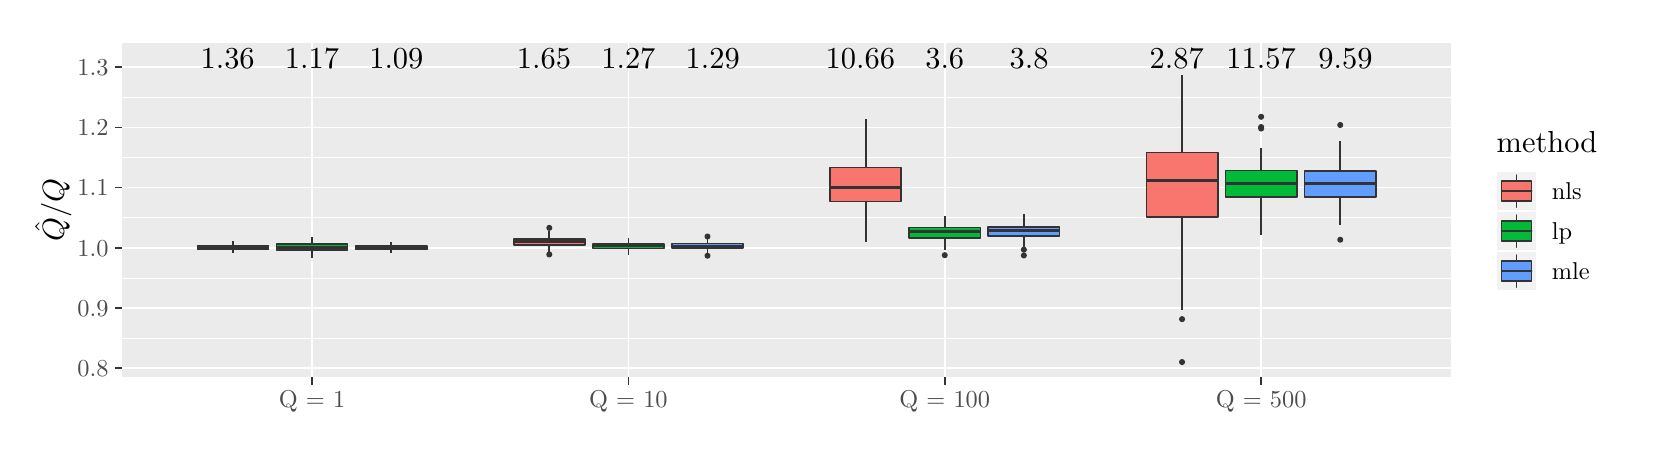
\begin{tikzpicture}[x=1pt,y=1pt]
\definecolor{fillColor}{RGB}{255,255,255}
\path[use as bounding box,fill=fillColor,fill opacity=0.00] (0,0) rectangle (578.16,144.54);
\begin{scope}
\path[clip] (  0.00,  0.00) rectangle (578.16,144.54);
\definecolor{drawColor}{RGB}{255,255,255}
\definecolor{fillColor}{RGB}{255,255,255}

\path[draw=drawColor,line width= 0.6pt,line join=round,line cap=round,fill=fillColor] (  0.00,  0.00) rectangle (578.16,144.54);
\end{scope}
\begin{scope}
\path[clip] ( 34.16, 18.22) rectangle (514.31,139.04);
\definecolor{fillColor}{gray}{0.92}

\path[fill=fillColor] ( 34.16, 18.22) rectangle (514.31,139.04);
\definecolor{drawColor}{RGB}{255,255,255}

\path[draw=drawColor,line width= 0.3pt,line join=round] ( 34.16, 32.36) --
	(514.31, 32.36);

\path[draw=drawColor,line width= 0.3pt,line join=round] ( 34.16, 54.11) --
	(514.31, 54.11);

\path[draw=drawColor,line width= 0.3pt,line join=round] ( 34.16, 75.87) --
	(514.31, 75.87);

\path[draw=drawColor,line width= 0.3pt,line join=round] ( 34.16, 97.63) --
	(514.31, 97.63);

\path[draw=drawColor,line width= 0.3pt,line join=round] ( 34.16,119.39) --
	(514.31,119.39);

\path[draw=drawColor,line width= 0.6pt,line join=round] ( 34.16, 21.48) --
	(514.31, 21.48);

\path[draw=drawColor,line width= 0.6pt,line join=round] ( 34.16, 43.23) --
	(514.31, 43.23);

\path[draw=drawColor,line width= 0.6pt,line join=round] ( 34.16, 64.99) --
	(514.31, 64.99);

\path[draw=drawColor,line width= 0.6pt,line join=round] ( 34.16, 86.75) --
	(514.31, 86.75);

\path[draw=drawColor,line width= 0.6pt,line join=round] ( 34.16,108.51) --
	(514.31,108.51);

\path[draw=drawColor,line width= 0.6pt,line join=round] ( 34.16,130.27) --
	(514.31,130.27);

\path[draw=drawColor,line width= 0.6pt,line join=round] (102.75, 18.22) --
	(102.75,139.04);

\path[draw=drawColor,line width= 0.6pt,line join=round] (217.07, 18.22) --
	(217.07,139.04);

\path[draw=drawColor,line width= 0.6pt,line join=round] (331.39, 18.22) --
	(331.39,139.04);

\path[draw=drawColor,line width= 0.6pt,line join=round] (445.71, 18.22) --
	(445.71,139.04);
\definecolor{drawColor}{gray}{0.20}

\path[draw=drawColor,line width= 0.6pt,line join=round] ( 74.17, 65.87) -- ( 74.17, 67.54);

\path[draw=drawColor,line width= 0.6pt,line join=round] ( 74.17, 64.38) -- ( 74.17, 62.98);
\definecolor{fillColor}{RGB}{248,118,109}

\path[draw=drawColor,line width= 0.6pt,line join=round,line cap=round,fill=fillColor] ( 61.31, 65.87) --
	( 61.31, 64.38) --
	( 87.03, 64.38) --
	( 87.03, 65.87) --
	( 61.31, 65.87) --
	cycle;

\path[draw=drawColor,line width= 1.1pt,line join=round] ( 61.31, 65.05) -- ( 87.03, 65.05);

\path[draw=drawColor,line width= 0.6pt,line join=round] (102.75, 66.26) -- (102.75, 68.74);

\path[draw=drawColor,line width= 0.6pt,line join=round] (102.75, 64.12) -- (102.75, 61.16);
\definecolor{fillColor}{RGB}{0,186,56}

\path[draw=drawColor,line width= 0.6pt,line join=round,line cap=round,fill=fillColor] ( 89.89, 66.26) --
	( 89.89, 64.12) --
	(115.61, 64.12) --
	(115.61, 66.26) --
	( 89.89, 66.26) --
	cycle;

\path[draw=drawColor,line width= 1.1pt,line join=round] ( 89.89, 65.12) -- (115.61, 65.12);

\path[draw=drawColor,line width= 0.6pt,line join=round] (131.33, 65.68) -- (131.33, 66.99);

\path[draw=drawColor,line width= 0.6pt,line join=round] (131.33, 64.43) -- (131.33, 63.21);
\definecolor{fillColor}{RGB}{97,156,255}

\path[draw=drawColor,line width= 0.6pt,line join=round,line cap=round,fill=fillColor] (118.47, 65.68) --
	(118.47, 64.43) --
	(144.19, 64.43) --
	(144.19, 65.68) --
	(118.47, 65.68) --
	cycle;

\path[draw=drawColor,line width= 1.1pt,line join=round] (118.47, 65.18) -- (144.19, 65.18);
\definecolor{fillColor}{gray}{0.20}

\path[draw=drawColor,line width= 0.4pt,line join=round,line cap=round,fill=fillColor] (188.49, 62.59) circle (  0.89);

\path[draw=drawColor,line width= 0.4pt,line join=round,line cap=round,fill=fillColor] (188.49, 72.20) circle (  0.89);

\path[draw=drawColor,line width= 0.6pt,line join=round] (188.49, 68.16) -- (188.49, 71.15);

\path[draw=drawColor,line width= 0.6pt,line join=round] (188.49, 65.99) -- (188.49, 63.11);
\definecolor{fillColor}{RGB}{248,118,109}

\path[draw=drawColor,line width= 0.6pt,line join=round,line cap=round,fill=fillColor] (175.63, 68.16) --
	(175.63, 65.99) --
	(201.35, 65.99) --
	(201.35, 68.16) --
	(175.63, 68.16) --
	cycle;

\path[draw=drawColor,line width= 1.1pt,line join=round] (175.63, 67.23) -- (201.35, 67.23);

\path[draw=drawColor,line width= 0.6pt,line join=round] (217.07, 66.43) -- (217.07, 68.56);

\path[draw=drawColor,line width= 0.6pt,line join=round] (217.07, 64.71) -- (217.07, 62.50);
\definecolor{fillColor}{RGB}{0,186,56}

\path[draw=drawColor,line width= 0.6pt,line join=round,line cap=round,fill=fillColor] (204.21, 66.43) --
	(204.21, 64.71) --
	(229.93, 64.71) --
	(229.93, 66.43) --
	(204.21, 66.43) --
	cycle;

\path[draw=drawColor,line width= 1.1pt,line join=round] (204.21, 65.68) -- (229.93, 65.68);
\definecolor{fillColor}{gray}{0.20}

\path[draw=drawColor,line width= 0.4pt,line join=round,line cap=round,fill=fillColor] (245.65, 69.08) circle (  0.89);

\path[draw=drawColor,line width= 0.4pt,line join=round,line cap=round,fill=fillColor] (245.65, 62.13) circle (  0.89);

\path[draw=drawColor,line width= 0.6pt,line join=round] (245.65, 66.61) -- (245.65, 68.76);

\path[draw=drawColor,line width= 0.6pt,line join=round] (245.65, 64.97) -- (245.65, 63.22);
\definecolor{fillColor}{RGB}{97,156,255}

\path[draw=drawColor,line width= 0.6pt,line join=round,line cap=round,fill=fillColor] (232.79, 66.61) --
	(232.79, 64.97) --
	(258.51, 64.97) --
	(258.51, 66.61) --
	(232.79, 66.61) --
	cycle;

\path[draw=drawColor,line width= 1.1pt,line join=round] (232.79, 65.63) -- (258.51, 65.63);

\path[draw=drawColor,line width= 0.6pt,line join=round] (302.81, 93.98) -- (302.81,111.48);

\path[draw=drawColor,line width= 0.6pt,line join=round] (302.81, 81.73) -- (302.81, 67.13);
\definecolor{fillColor}{RGB}{248,118,109}

\path[draw=drawColor,line width= 0.6pt,line join=round,line cap=round,fill=fillColor] (289.95, 93.98) --
	(289.95, 81.73) --
	(315.67, 81.73) --
	(315.67, 93.98) --
	(289.95, 93.98) --
	cycle;

\path[draw=drawColor,line width= 1.1pt,line join=round] (289.95, 86.92) -- (315.67, 86.92);
\definecolor{fillColor}{gray}{0.20}

\path[draw=drawColor,line width= 0.4pt,line join=round,line cap=round,fill=fillColor] (331.39, 62.33) circle (  0.89);

\path[draw=drawColor,line width= 0.6pt,line join=round] (331.39, 72.36) -- (331.39, 76.37);

\path[draw=drawColor,line width= 0.6pt,line join=round] (331.39, 68.54) -- (331.39, 64.12);
\definecolor{fillColor}{RGB}{0,186,56}

\path[draw=drawColor,line width= 0.6pt,line join=round,line cap=round,fill=fillColor] (318.53, 72.36) --
	(318.53, 68.54) --
	(344.25, 68.54) --
	(344.25, 72.36) --
	(318.53, 72.36) --
	cycle;

\path[draw=drawColor,line width= 1.1pt,line join=round] (318.53, 70.98) -- (344.25, 70.98);
\definecolor{fillColor}{gray}{0.20}

\path[draw=drawColor,line width= 0.4pt,line join=round,line cap=round,fill=fillColor] (359.97, 64.32) circle (  0.89);

\path[draw=drawColor,line width= 0.4pt,line join=round,line cap=round,fill=fillColor] (359.97, 62.23) circle (  0.89);

\path[draw=drawColor,line width= 0.6pt,line join=round] (359.97, 72.50) -- (359.97, 77.26);

\path[draw=drawColor,line width= 0.6pt,line join=round] (359.97, 69.28) -- (359.97, 64.55);
\definecolor{fillColor}{RGB}{97,156,255}

\path[draw=drawColor,line width= 0.6pt,line join=round,line cap=round,fill=fillColor] (347.11, 72.50) --
	(347.11, 69.28) --
	(372.83, 69.28) --
	(372.83, 72.50) --
	(347.11, 72.50) --
	cycle;

\path[draw=drawColor,line width= 1.1pt,line join=round] (347.11, 71.26) -- (372.83, 71.26);
\definecolor{fillColor}{gray}{0.20}

\path[draw=drawColor,line width= 0.4pt,line join=round,line cap=round,fill=fillColor] (417.13, 39.21) circle (  0.89);

\path[draw=drawColor,line width= 0.4pt,line join=round,line cap=round,fill=fillColor] (417.13, 23.71) circle (  0.89);

\path[draw=drawColor,line width= 0.6pt,line join=round] (417.13, 99.47) -- (417.13,127.32);

\path[draw=drawColor,line width= 0.6pt,line join=round] (417.13, 76.06) -- (417.13, 42.40);
\definecolor{fillColor}{RGB}{248,118,109}

\path[draw=drawColor,line width= 0.6pt,line join=round,line cap=round,fill=fillColor] (404.27, 99.47) --
	(404.27, 76.06) --
	(430.00, 76.06) --
	(430.00, 99.47) --
	(404.27, 99.47) --
	cycle;

\path[draw=drawColor,line width= 1.1pt,line join=round] (404.27, 89.42) -- (430.00, 89.42);
\definecolor{fillColor}{gray}{0.20}

\path[draw=drawColor,line width= 0.4pt,line join=round,line cap=round,fill=fillColor] (445.71,108.63) circle (  0.89);

\path[draw=drawColor,line width= 0.4pt,line join=round,line cap=round,fill=fillColor] (445.71,108.09) circle (  0.89);

\path[draw=drawColor,line width= 0.4pt,line join=round,line cap=round,fill=fillColor] (445.71,112.34) circle (  0.89);

\path[draw=drawColor,line width= 0.6pt,line join=round] (445.71, 92.89) -- (445.71,101.08);

\path[draw=drawColor,line width= 0.6pt,line join=round] (445.71, 83.32) -- (445.71, 69.52);
\definecolor{fillColor}{RGB}{0,186,56}

\path[draw=drawColor,line width= 0.6pt,line join=round,line cap=round,fill=fillColor] (432.85, 92.89) --
	(432.85, 83.32) --
	(458.58, 83.32) --
	(458.58, 92.89) --
	(432.85, 92.89) --
	cycle;

\path[draw=drawColor,line width= 1.1pt,line join=round] (432.85, 88.29) -- (458.58, 88.29);
\definecolor{fillColor}{gray}{0.20}

\path[draw=drawColor,line width= 0.4pt,line join=round,line cap=round,fill=fillColor] (474.29, 67.91) circle (  0.89);

\path[draw=drawColor,line width= 0.4pt,line join=round,line cap=round,fill=fillColor] (474.29,109.37) circle (  0.89);

\path[draw=drawColor,line width= 0.6pt,line join=round] (474.29, 92.85) -- (474.29,103.73);

\path[draw=drawColor,line width= 0.6pt,line join=round] (474.29, 83.33) -- (474.29, 73.30);
\definecolor{fillColor}{RGB}{97,156,255}

\path[draw=drawColor,line width= 0.6pt,line join=round,line cap=round,fill=fillColor] (461.43, 92.85) --
	(461.43, 83.33) --
	(487.16, 83.33) --
	(487.16, 92.85) --
	(461.43, 92.85) --
	cycle;

\path[draw=drawColor,line width= 1.1pt,line join=round] (461.43, 88.32) -- (487.16, 88.32);
\definecolor{drawColor}{RGB}{0,0,0}

\node[text=drawColor,anchor=base,inner sep=0pt, outer sep=0pt, scale=  1.10] at (133.23,129.75) {1.09};

\node[text=drawColor,anchor=base,inner sep=0pt, outer sep=0pt, scale=  1.10] at (102.75,129.75) {1.17};

\node[text=drawColor,anchor=base,inner sep=0pt, outer sep=0pt, scale=  1.10] at ( 72.26,129.75) {1.36};

\node[text=drawColor,anchor=base,inner sep=0pt, outer sep=0pt, scale=  1.10] at (247.56,129.75) {1.29};

\node[text=drawColor,anchor=base,inner sep=0pt, outer sep=0pt, scale=  1.10] at (217.07,129.75) {1.27};

\node[text=drawColor,anchor=base,inner sep=0pt, outer sep=0pt, scale=  1.10] at (186.59,129.75) {1.65};

\node[text=drawColor,anchor=base,inner sep=0pt, outer sep=0pt, scale=  1.10] at (361.88,129.75) {3.8};

\node[text=drawColor,anchor=base,inner sep=0pt, outer sep=0pt, scale=  1.10] at (331.39,129.75) {3.6};

\node[text=drawColor,anchor=base,inner sep=0pt, outer sep=0pt, scale=  1.10] at (300.91,129.75) {10.66};

\node[text=drawColor,anchor=base,inner sep=0pt, outer sep=0pt, scale=  1.10] at (476.20,129.75) {9.59};

\node[text=drawColor,anchor=base,inner sep=0pt, outer sep=0pt, scale=  1.10] at (445.71,129.75) {11.57};

\node[text=drawColor,anchor=base,inner sep=0pt, outer sep=0pt, scale=  1.10] at (415.23,129.75) {2.87};
\end{scope}
\begin{scope}
\path[clip] (  0.00,  0.00) rectangle (578.16,144.54);
\definecolor{drawColor}{gray}{0.30}

\node[text=drawColor,anchor=base east,inner sep=0pt, outer sep=0pt, scale=  0.88] at ( 29.21, 18.44) {0.8};

\node[text=drawColor,anchor=base east,inner sep=0pt, outer sep=0pt, scale=  0.88] at ( 29.21, 40.20) {0.9};

\node[text=drawColor,anchor=base east,inner sep=0pt, outer sep=0pt, scale=  0.88] at ( 29.21, 61.96) {1.0};

\node[text=drawColor,anchor=base east,inner sep=0pt, outer sep=0pt, scale=  0.88] at ( 29.21, 83.72) {1.1};

\node[text=drawColor,anchor=base east,inner sep=0pt, outer sep=0pt, scale=  0.88] at ( 29.21,105.48) {1.2};

\node[text=drawColor,anchor=base east,inner sep=0pt, outer sep=0pt, scale=  0.88] at ( 29.21,127.24) {1.3};
\end{scope}
\begin{scope}
\path[clip] (  0.00,  0.00) rectangle (578.16,144.54);
\definecolor{drawColor}{gray}{0.20}

\path[draw=drawColor,line width= 0.6pt,line join=round] ( 31.41, 21.48) --
	( 34.16, 21.48);

\path[draw=drawColor,line width= 0.6pt,line join=round] ( 31.41, 43.23) --
	( 34.16, 43.23);

\path[draw=drawColor,line width= 0.6pt,line join=round] ( 31.41, 64.99) --
	( 34.16, 64.99);

\path[draw=drawColor,line width= 0.6pt,line join=round] ( 31.41, 86.75) --
	( 34.16, 86.75);

\path[draw=drawColor,line width= 0.6pt,line join=round] ( 31.41,108.51) --
	( 34.16,108.51);

\path[draw=drawColor,line width= 0.6pt,line join=round] ( 31.41,130.27) --
	( 34.16,130.27);
\end{scope}
\begin{scope}
\path[clip] (  0.00,  0.00) rectangle (578.16,144.54);
\definecolor{drawColor}{gray}{0.20}

\path[draw=drawColor,line width= 0.6pt,line join=round] (102.75, 15.47) --
	(102.75, 18.22);

\path[draw=drawColor,line width= 0.6pt,line join=round] (217.07, 15.47) --
	(217.07, 18.22);

\path[draw=drawColor,line width= 0.6pt,line join=round] (331.39, 15.47) --
	(331.39, 18.22);

\path[draw=drawColor,line width= 0.6pt,line join=round] (445.71, 15.47) --
	(445.71, 18.22);
\end{scope}
\begin{scope}
\path[clip] (  0.00,  0.00) rectangle (578.16,144.54);
\definecolor{drawColor}{gray}{0.30}

\node[text=drawColor,anchor=base,inner sep=0pt, outer sep=0pt, scale=  0.88] at (102.75,  7.21) {Q = 1};

\node[text=drawColor,anchor=base,inner sep=0pt, outer sep=0pt, scale=  0.88] at (217.07,  7.21) {Q = 10};

\node[text=drawColor,anchor=base,inner sep=0pt, outer sep=0pt, scale=  0.88] at (331.39,  7.21) {Q = 100};

\node[text=drawColor,anchor=base,inner sep=0pt, outer sep=0pt, scale=  0.88] at (445.71,  7.21) {Q = 500};
\end{scope}
\begin{scope}
\path[clip] (  0.00,  0.00) rectangle (578.16,144.54);
\definecolor{drawColor}{RGB}{0,0,0}

\node[text=drawColor,rotate= 90.00,anchor=base,inner sep=0pt, outer sep=0pt, scale=  1.10] at ( 13.08, 78.63) {$\hat{Q}/Q$};
\end{scope}
\begin{scope}
\path[clip] (  0.00,  0.00) rectangle (578.16,144.54);
\definecolor{fillColor}{RGB}{255,255,255}

\path[fill=fillColor] (525.31, 43.84) rectangle (572.66,113.42);
\end{scope}
\begin{scope}
\path[clip] (  0.00,  0.00) rectangle (578.16,144.54);
\definecolor{drawColor}{RGB}{0,0,0}

\node[text=drawColor,anchor=base west,inner sep=0pt, outer sep=0pt, scale=  1.10] at (530.81, 99.27) {method};
\end{scope}
\begin{scope}
\path[clip] (  0.00,  0.00) rectangle (578.16,144.54);
\definecolor{drawColor}{RGB}{255,255,255}
\definecolor{fillColor}{gray}{0.95}

\path[draw=drawColor,line width= 0.6pt,line join=round,line cap=round,fill=fillColor] (530.81, 78.25) rectangle (545.26, 92.70);
\end{scope}
\begin{scope}
\path[clip] (  0.00,  0.00) rectangle (578.16,144.54);
\definecolor{drawColor}{gray}{0.20}

\path[draw=drawColor,line width= 0.6pt,line join=round,line cap=round] (538.03, 79.70) --
	(538.03, 81.86);

\path[draw=drawColor,line width= 0.6pt,line join=round,line cap=round] (538.03, 89.09) --
	(538.03, 91.26);
\definecolor{fillColor}{RGB}{248,118,109}

\path[draw=drawColor,line width= 0.6pt,line join=round,line cap=round,fill=fillColor] (532.61, 81.86) rectangle (543.45, 89.09);

\path[draw=drawColor,line width= 0.6pt,line join=round,line cap=round] (532.61, 85.48) --
	(543.45, 85.48);
\end{scope}
\begin{scope}
\path[clip] (  0.00,  0.00) rectangle (578.16,144.54);
\definecolor{drawColor}{RGB}{255,255,255}
\definecolor{fillColor}{gray}{0.95}

\path[draw=drawColor,line width= 0.6pt,line join=round,line cap=round,fill=fillColor] (530.81, 63.80) rectangle (545.26, 78.25);
\end{scope}
\begin{scope}
\path[clip] (  0.00,  0.00) rectangle (578.16,144.54);
\definecolor{drawColor}{gray}{0.20}

\path[draw=drawColor,line width= 0.6pt,line join=round,line cap=round] (538.03, 65.24) --
	(538.03, 67.41);

\path[draw=drawColor,line width= 0.6pt,line join=round,line cap=round] (538.03, 74.64) --
	(538.03, 76.81);
\definecolor{fillColor}{RGB}{0,186,56}

\path[draw=drawColor,line width= 0.6pt,line join=round,line cap=round,fill=fillColor] (532.61, 67.41) rectangle (543.45, 74.64);

\path[draw=drawColor,line width= 0.6pt,line join=round,line cap=round] (532.61, 71.02) --
	(543.45, 71.02);
\end{scope}
\begin{scope}
\path[clip] (  0.00,  0.00) rectangle (578.16,144.54);
\definecolor{drawColor}{RGB}{255,255,255}
\definecolor{fillColor}{gray}{0.95}

\path[draw=drawColor,line width= 0.6pt,line join=round,line cap=round,fill=fillColor] (530.81, 49.34) rectangle (545.26, 63.80);
\end{scope}
\begin{scope}
\path[clip] (  0.00,  0.00) rectangle (578.16,144.54);
\definecolor{drawColor}{gray}{0.20}

\path[draw=drawColor,line width= 0.6pt,line join=round,line cap=round] (538.03, 50.79) --
	(538.03, 52.96);

\path[draw=drawColor,line width= 0.6pt,line join=round,line cap=round] (538.03, 60.18) --
	(538.03, 62.35);
\definecolor{fillColor}{RGB}{97,156,255}

\path[draw=drawColor,line width= 0.6pt,line join=round,line cap=round,fill=fillColor] (532.61, 52.96) rectangle (543.45, 60.18);

\path[draw=drawColor,line width= 0.6pt,line join=round,line cap=round] (532.61, 56.57) --
	(543.45, 56.57);
\end{scope}
\begin{scope}
\path[clip] (  0.00,  0.00) rectangle (578.16,144.54);
\definecolor{drawColor}{RGB}{0,0,0}

\node[text=drawColor,anchor=base west,inner sep=0pt, outer sep=0pt, scale=  0.88] at (550.76, 82.45) {nls};
\end{scope}
\begin{scope}
\path[clip] (  0.00,  0.00) rectangle (578.16,144.54);
\definecolor{drawColor}{RGB}{0,0,0}

\node[text=drawColor,anchor=base west,inner sep=0pt, outer sep=0pt, scale=  0.88] at (550.76, 67.99) {lp};
\end{scope}
\begin{scope}
\path[clip] (  0.00,  0.00) rectangle (578.16,144.54);
\definecolor{drawColor}{RGB}{0,0,0}

\node[text=drawColor,anchor=base west,inner sep=0pt, outer sep=0pt, scale=  0.88] at (550.76, 53.54) {mle};
\end{scope}
\end{tikzpicture}
}
  \end{subfigure}
  \hfill
  \begin{subfigure}
    \centering
    \resizebox{1.1\linewidth}{!}{% Created by tikzDevice version 0.12.3 on 2019-09-30 10:38:11
% !TEX encoding = UTF-8 Unicode
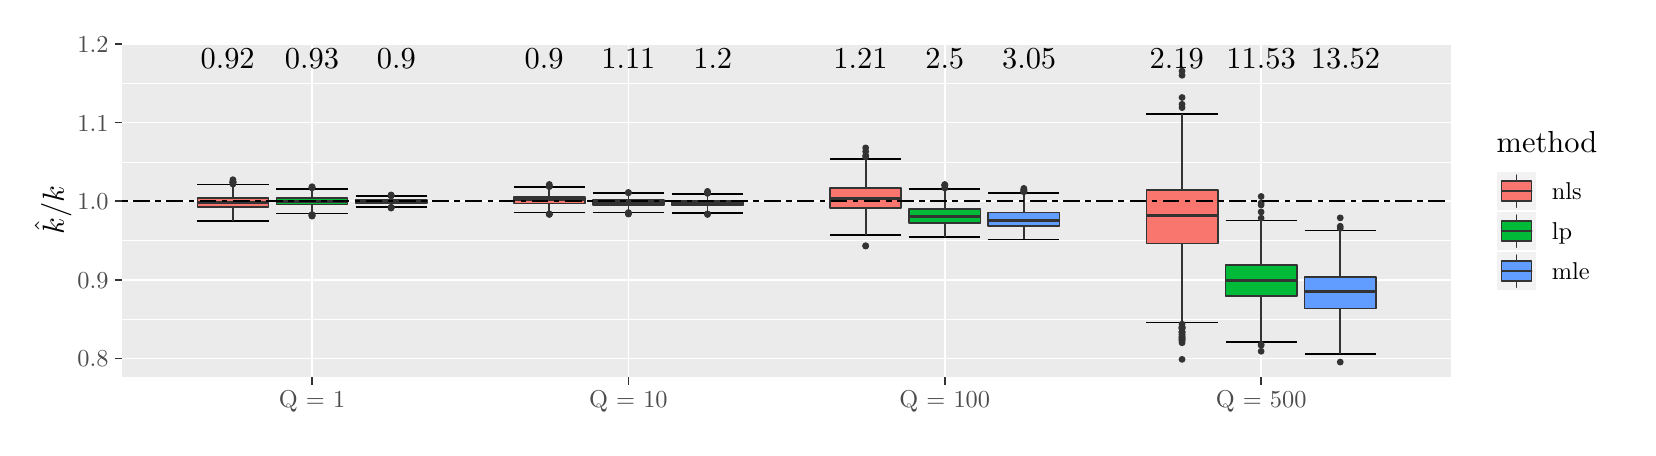
\begin{tikzpicture}[x=1pt,y=1pt]
\definecolor{fillColor}{RGB}{255,255,255}
\path[use as bounding box,fill=fillColor,fill opacity=0.00] (0,0) rectangle (578.16,144.54);
\begin{scope}
\path[clip] (  0.00,  0.00) rectangle (578.16,144.54);
\definecolor{drawColor}{RGB}{255,255,255}
\definecolor{fillColor}{RGB}{255,255,255}

\path[draw=drawColor,line width= 0.6pt,line join=round,line cap=round,fill=fillColor] (  0.00,  0.00) rectangle (578.16,144.54);
\end{scope}
\begin{scope}
\path[clip] ( 34.16, 18.22) rectangle (514.31,139.04);
\definecolor{fillColor}{gray}{0.92}

\path[fill=fillColor] ( 34.16, 18.22) rectangle (514.31,139.04);
\definecolor{drawColor}{RGB}{255,255,255}

\path[draw=drawColor,line width= 0.3pt,line join=round] ( 34.16, 39.18) --
	(514.31, 39.18);

\path[draw=drawColor,line width= 0.3pt,line join=round] ( 34.16, 67.60) --
	(514.31, 67.60);

\path[draw=drawColor,line width= 0.3pt,line join=round] ( 34.16, 96.01) --
	(514.31, 96.01);

\path[draw=drawColor,line width= 0.3pt,line join=round] ( 34.16,124.42) --
	(514.31,124.42);

\path[draw=drawColor,line width= 0.6pt,line join=round] ( 34.16, 24.98) --
	(514.31, 24.98);

\path[draw=drawColor,line width= 0.6pt,line join=round] ( 34.16, 53.39) --
	(514.31, 53.39);

\path[draw=drawColor,line width= 0.6pt,line join=round] ( 34.16, 81.80) --
	(514.31, 81.80);

\path[draw=drawColor,line width= 0.6pt,line join=round] ( 34.16,110.22) --
	(514.31,110.22);

\path[draw=drawColor,line width= 0.6pt,line join=round] ( 34.16,138.63) --
	(514.31,138.63);

\path[draw=drawColor,line width= 0.6pt,line join=round] (102.75, 18.22) --
	(102.75,139.04);

\path[draw=drawColor,line width= 0.6pt,line join=round] (217.07, 18.22) --
	(217.07,139.04);

\path[draw=drawColor,line width= 0.6pt,line join=round] (331.39, 18.22) --
	(331.39,139.04);

\path[draw=drawColor,line width= 0.6pt,line join=round] (445.71, 18.22) --
	(445.71,139.04);
\definecolor{drawColor}{RGB}{0,0,0}

\path[draw=drawColor,line width= 0.6pt,line join=round] ( 61.31, 87.90) --
	( 87.03, 87.90);

\path[draw=drawColor,line width= 0.6pt,line join=round] ( 74.17, 87.90) --
	( 74.17, 74.79);

\path[draw=drawColor,line width= 0.6pt,line join=round] ( 61.31, 74.79) --
	( 87.03, 74.79);

\path[draw=drawColor,line width= 0.6pt,line join=round] ( 89.89, 86.33) --
	(115.61, 86.33);

\path[draw=drawColor,line width= 0.6pt,line join=round] (102.75, 86.33) --
	(102.75, 77.39);

\path[draw=drawColor,line width= 0.6pt,line join=round] ( 89.89, 77.39) --
	(115.61, 77.39);

\path[draw=drawColor,line width= 0.6pt,line join=round] (118.47, 83.67) --
	(144.19, 83.67);

\path[draw=drawColor,line width= 0.6pt,line join=round] (131.33, 83.67) --
	(131.33, 79.68);

\path[draw=drawColor,line width= 0.6pt,line join=round] (118.47, 79.68) --
	(144.19, 79.68);

\path[draw=drawColor,line width= 0.6pt,line join=round] (175.63, 87.02) --
	(201.35, 87.02);

\path[draw=drawColor,line width= 0.6pt,line join=round] (188.49, 87.02) --
	(188.49, 77.72);

\path[draw=drawColor,line width= 0.6pt,line join=round] (175.63, 77.72) --
	(201.35, 77.72);

\path[draw=drawColor,line width= 0.6pt,line join=round] (204.21, 84.72) --
	(229.93, 84.72);

\path[draw=drawColor,line width= 0.6pt,line join=round] (217.07, 84.72) --
	(217.07, 77.79);

\path[draw=drawColor,line width= 0.6pt,line join=round] (204.21, 77.79) --
	(229.93, 77.79);

\path[draw=drawColor,line width= 0.6pt,line join=round] (232.79, 84.46) --
	(258.51, 84.46);

\path[draw=drawColor,line width= 0.6pt,line join=round] (245.65, 84.46) --
	(245.65, 77.64);

\path[draw=drawColor,line width= 0.6pt,line join=round] (232.79, 77.64) --
	(258.51, 77.64);

\path[draw=drawColor,line width= 0.6pt,line join=round] (289.95, 97.11) --
	(315.67, 97.11);

\path[draw=drawColor,line width= 0.6pt,line join=round] (302.81, 97.11) --
	(302.81, 69.55);

\path[draw=drawColor,line width= 0.6pt,line join=round] (289.95, 69.55) --
	(315.67, 69.55);

\path[draw=drawColor,line width= 0.6pt,line join=round] (318.53, 86.15) --
	(344.25, 86.15);

\path[draw=drawColor,line width= 0.6pt,line join=round] (331.39, 86.15) --
	(331.39, 68.79);

\path[draw=drawColor,line width= 0.6pt,line join=round] (318.53, 68.79) --
	(344.25, 68.79);

\path[draw=drawColor,line width= 0.6pt,line join=round] (347.11, 84.72) --
	(372.83, 84.72);

\path[draw=drawColor,line width= 0.6pt,line join=round] (359.97, 84.72) --
	(359.97, 68.02);

\path[draw=drawColor,line width= 0.6pt,line join=round] (347.11, 68.02) --
	(372.83, 68.02);

\path[draw=drawColor,line width= 0.6pt,line join=round] (404.27,113.28) --
	(430.00,113.28);

\path[draw=drawColor,line width= 0.6pt,line join=round] (417.13,113.28) --
	(417.13, 38.06);

\path[draw=drawColor,line width= 0.6pt,line join=round] (404.27, 38.06) --
	(430.00, 38.06);

\path[draw=drawColor,line width= 0.6pt,line join=round] (432.85, 74.82) --
	(458.58, 74.82);

\path[draw=drawColor,line width= 0.6pt,line join=round] (445.71, 74.82) --
	(445.71, 30.94);

\path[draw=drawColor,line width= 0.6pt,line join=round] (432.85, 30.94) --
	(458.58, 30.94);

\path[draw=drawColor,line width= 0.6pt,line join=round] (461.43, 71.20) --
	(487.16, 71.20);

\path[draw=drawColor,line width= 0.6pt,line join=round] (474.29, 71.20) --
	(474.29, 26.65);

\path[draw=drawColor,line width= 0.6pt,line join=round] (461.43, 26.65) --
	(487.16, 26.65);
\definecolor{drawColor}{gray}{0.20}
\definecolor{fillColor}{gray}{0.20}

\path[draw=drawColor,line width= 0.4pt,line join=round,line cap=round,fill=fillColor] ( 74.17, 88.78) circle (  1.02);

\path[draw=drawColor,line width= 0.4pt,line join=round,line cap=round,fill=fillColor] ( 74.17, 88.79) circle (  1.02);

\path[draw=drawColor,line width= 0.4pt,line join=round,line cap=round,fill=fillColor] ( 74.17, 88.02) circle (  1.02);

\path[draw=drawColor,line width= 0.4pt,line join=round,line cap=round,fill=fillColor] ( 74.17, 88.52) circle (  1.02);

\path[draw=drawColor,line width= 0.4pt,line join=round,line cap=round,fill=fillColor] ( 74.17, 89.60) circle (  1.02);

\path[draw=drawColor,line width= 0.4pt,line join=round,line cap=round,fill=fillColor] ( 74.17, 88.91) circle (  1.02);

\path[draw=drawColor,line width= 0.4pt,line join=round,line cap=round,fill=fillColor] ( 74.17, 88.61) circle (  1.02);

\path[draw=drawColor,line width= 0.6pt,line join=round] ( 74.17, 83.00) -- ( 74.17, 87.90);

\path[draw=drawColor,line width= 0.6pt,line join=round] ( 74.17, 79.67) -- ( 74.17, 74.79);
\definecolor{fillColor}{RGB}{248,118,109}

\path[draw=drawColor,line width= 0.6pt,line join=round,line cap=round,fill=fillColor] ( 61.31, 83.00) --
	( 61.31, 79.67) --
	( 87.03, 79.67) --
	( 87.03, 83.00) --
	( 61.31, 83.00) --
	cycle;

\path[draw=drawColor,line width= 1.1pt,line join=round] ( 61.31, 81.28) -- ( 87.03, 81.28);
\definecolor{fillColor}{gray}{0.20}

\path[draw=drawColor,line width= 0.4pt,line join=round,line cap=round,fill=fillColor] (102.75, 76.59) circle (  1.02);

\path[draw=drawColor,line width= 0.4pt,line join=round,line cap=round,fill=fillColor] (102.75, 77.00) circle (  1.02);

\path[draw=drawColor,line width= 0.4pt,line join=round,line cap=round,fill=fillColor] (102.75, 76.83) circle (  1.02);

\path[draw=drawColor,line width= 0.4pt,line join=round,line cap=round,fill=fillColor] (102.75, 86.85) circle (  1.02);

\path[draw=drawColor,line width= 0.4pt,line join=round,line cap=round,fill=fillColor] (102.75, 76.56) circle (  1.02);

\path[draw=drawColor,line width= 0.4pt,line join=round,line cap=round,fill=fillColor] (102.75, 87.07) circle (  1.02);

\path[draw=drawColor,line width= 0.4pt,line join=round,line cap=round,fill=fillColor] (102.75, 76.45) circle (  1.02);

\path[draw=drawColor,line width= 0.4pt,line join=round,line cap=round,fill=fillColor] (102.75, 86.64) circle (  1.02);

\path[draw=drawColor,line width= 0.6pt,line join=round] (102.75, 82.98) -- (102.75, 86.33);

\path[draw=drawColor,line width= 0.6pt,line join=round] (102.75, 80.65) -- (102.75, 77.39);
\definecolor{fillColor}{RGB}{0,186,56}

\path[draw=drawColor,line width= 0.6pt,line join=round,line cap=round,fill=fillColor] ( 89.89, 82.98) --
	( 89.89, 80.65) --
	(115.61, 80.65) --
	(115.61, 82.98) --
	( 89.89, 82.98) --
	cycle;

\path[draw=drawColor,line width= 1.1pt,line join=round] ( 89.89, 81.70) -- (115.61, 81.70);
\definecolor{fillColor}{gray}{0.20}

\path[draw=drawColor,line width= 0.4pt,line join=round,line cap=round,fill=fillColor] (131.33, 84.04) circle (  1.02);

\path[draw=drawColor,line width= 0.4pt,line join=round,line cap=round,fill=fillColor] (131.33, 79.60) circle (  1.02);

\path[draw=drawColor,line width= 0.4pt,line join=round,line cap=round,fill=fillColor] (131.33, 83.76) circle (  1.02);

\path[draw=drawColor,line width= 0.4pt,line join=round,line cap=round,fill=fillColor] (131.33, 84.05) circle (  1.02);

\path[draw=drawColor,line width= 0.4pt,line join=round,line cap=round,fill=fillColor] (131.33, 79.50) circle (  1.02);

\path[draw=drawColor,line width= 0.4pt,line join=round,line cap=round,fill=fillColor] (131.33, 79.34) circle (  1.02);

\path[draw=drawColor,line width= 0.4pt,line join=round,line cap=round,fill=fillColor] (131.33, 83.84) circle (  1.02);

\path[draw=drawColor,line width= 0.4pt,line join=round,line cap=round,fill=fillColor] (131.33, 79.58) circle (  1.02);

\path[draw=drawColor,line width= 0.6pt,line join=round] (131.33, 82.18) -- (131.33, 83.67);

\path[draw=drawColor,line width= 0.6pt,line join=round] (131.33, 81.18) -- (131.33, 79.68);
\definecolor{fillColor}{RGB}{97,156,255}

\path[draw=drawColor,line width= 0.6pt,line join=round,line cap=round,fill=fillColor] (118.47, 82.18) --
	(118.47, 81.18) --
	(144.19, 81.18) --
	(144.19, 82.18) --
	(118.47, 82.18) --
	cycle;

\path[draw=drawColor,line width= 1.1pt,line join=round] (118.47, 81.70) -- (144.19, 81.70);
\definecolor{fillColor}{gray}{0.20}

\path[draw=drawColor,line width= 0.4pt,line join=round,line cap=round,fill=fillColor] (188.49, 77.20) circle (  1.02);

\path[draw=drawColor,line width= 0.4pt,line join=round,line cap=round,fill=fillColor] (188.49, 87.35) circle (  1.02);

\path[draw=drawColor,line width= 0.4pt,line join=round,line cap=round,fill=fillColor] (188.49, 87.18) circle (  1.02);

\path[draw=drawColor,line width= 0.4pt,line join=round,line cap=round,fill=fillColor] (188.49, 87.13) circle (  1.02);

\path[draw=drawColor,line width= 0.4pt,line join=round,line cap=round,fill=fillColor] (188.49, 77.13) circle (  1.02);

\path[draw=drawColor,line width= 0.4pt,line join=round,line cap=round,fill=fillColor] (188.49, 87.88) circle (  1.02);

\path[draw=drawColor,line width= 0.4pt,line join=round,line cap=round,fill=fillColor] (188.49, 77.07) circle (  1.02);

\path[draw=drawColor,line width= 0.6pt,line join=round] (188.49, 83.40) -- (188.49, 87.02);

\path[draw=drawColor,line width= 0.6pt,line join=round] (188.49, 80.97) -- (188.49, 77.72);
\definecolor{fillColor}{RGB}{248,118,109}

\path[draw=drawColor,line width= 0.6pt,line join=round,line cap=round,fill=fillColor] (175.63, 83.40) --
	(175.63, 80.97) --
	(201.35, 80.97) --
	(201.35, 83.40) --
	(175.63, 83.40) --
	cycle;

\path[draw=drawColor,line width= 1.1pt,line join=round] (175.63, 82.30) -- (201.35, 82.30);
\definecolor{fillColor}{gray}{0.20}

\path[draw=drawColor,line width= 0.4pt,line join=round,line cap=round,fill=fillColor] (217.07, 84.99) circle (  1.02);

\path[draw=drawColor,line width= 0.4pt,line join=round,line cap=round,fill=fillColor] (217.07, 77.18) circle (  1.02);

\path[draw=drawColor,line width= 0.4pt,line join=round,line cap=round,fill=fillColor] (217.07, 77.34) circle (  1.02);

\path[draw=drawColor,line width= 0.4pt,line join=round,line cap=round,fill=fillColor] (217.07, 77.63) circle (  1.02);

\path[draw=drawColor,line width= 0.4pt,line join=round,line cap=round,fill=fillColor] (217.07, 77.69) circle (  1.02);

\path[draw=drawColor,line width= 0.4pt,line join=round,line cap=round,fill=fillColor] (217.07, 84.86) circle (  1.02);

\path[draw=drawColor,line width= 0.6pt,line join=round] (217.07, 82.18) -- (217.07, 84.72);

\path[draw=drawColor,line width= 0.6pt,line join=round] (217.07, 80.41) -- (217.07, 77.79);
\definecolor{fillColor}{RGB}{0,186,56}

\path[draw=drawColor,line width= 0.6pt,line join=round,line cap=round,fill=fillColor] (204.21, 82.18) --
	(204.21, 80.41) --
	(229.93, 80.41) --
	(229.93, 82.18) --
	(204.21, 82.18) --
	cycle;

\path[draw=drawColor,line width= 1.1pt,line join=round] (204.21, 81.33) -- (229.93, 81.33);
\definecolor{fillColor}{gray}{0.20}

\path[draw=drawColor,line width= 0.4pt,line join=round,line cap=round,fill=fillColor] (245.65, 85.38) circle (  1.02);

\path[draw=drawColor,line width= 0.4pt,line join=round,line cap=round,fill=fillColor] (245.65, 77.05) circle (  1.02);

\path[draw=drawColor,line width= 0.4pt,line join=round,line cap=round,fill=fillColor] (245.65, 77.23) circle (  1.02);

\path[draw=drawColor,line width= 0.4pt,line join=round,line cap=round,fill=fillColor] (245.65, 84.68) circle (  1.02);

\path[draw=drawColor,line width= 0.4pt,line join=round,line cap=round,fill=fillColor] (245.65, 84.76) circle (  1.02);

\path[draw=drawColor,line width= 0.6pt,line join=round] (245.65, 82.01) -- (245.65, 84.46);

\path[draw=drawColor,line width= 0.6pt,line join=round] (245.65, 80.23) -- (245.65, 77.64);
\definecolor{fillColor}{RGB}{97,156,255}

\path[draw=drawColor,line width= 0.6pt,line join=round,line cap=round,fill=fillColor] (232.79, 82.01) --
	(232.79, 80.23) --
	(258.51, 80.23) --
	(258.51, 82.01) --
	(232.79, 82.01) --
	cycle;

\path[draw=drawColor,line width= 1.1pt,line join=round] (232.79, 81.09) -- (258.51, 81.09);
\definecolor{fillColor}{gray}{0.20}

\path[draw=drawColor,line width= 0.4pt,line join=round,line cap=round,fill=fillColor] (302.81,101.11) circle (  1.02);

\path[draw=drawColor,line width= 0.4pt,line join=round,line cap=round,fill=fillColor] (302.81, 97.85) circle (  1.02);

\path[draw=drawColor,line width= 0.4pt,line join=round,line cap=round,fill=fillColor] (302.81, 99.77) circle (  1.02);

\path[draw=drawColor,line width= 0.4pt,line join=round,line cap=round,fill=fillColor] (302.81, 65.64) circle (  1.02);

\path[draw=drawColor,line width= 0.4pt,line join=round,line cap=round,fill=fillColor] (302.81, 98.32) circle (  1.02);

\path[draw=drawColor,line width= 0.4pt,line join=round,line cap=round,fill=fillColor] (302.81, 65.73) circle (  1.02);

\path[draw=drawColor,line width= 0.6pt,line join=round] (302.81, 86.49) -- (302.81, 97.11);

\path[draw=drawColor,line width= 0.6pt,line join=round] (302.81, 79.35) -- (302.81, 69.55);
\definecolor{fillColor}{RGB}{248,118,109}

\path[draw=drawColor,line width= 0.6pt,line join=round,line cap=round,fill=fillColor] (289.95, 86.49) --
	(289.95, 79.35) --
	(315.67, 79.35) --
	(315.67, 86.49) --
	(289.95, 86.49) --
	cycle;

\path[draw=drawColor,line width= 1.1pt,line join=round] (289.95, 82.84) -- (315.67, 82.84);
\definecolor{fillColor}{gray}{0.20}

\path[draw=drawColor,line width= 0.4pt,line join=round,line cap=round,fill=fillColor] (331.39, 87.54) circle (  1.02);

\path[draw=drawColor,line width= 0.4pt,line join=round,line cap=round,fill=fillColor] (331.39, 87.87) circle (  1.02);

\path[draw=drawColor,line width= 0.4pt,line join=round,line cap=round,fill=fillColor] (331.39, 87.57) circle (  1.02);

\path[draw=drawColor,line width= 0.4pt,line join=round,line cap=round,fill=fillColor] (331.39, 86.59) circle (  1.02);

\path[draw=drawColor,line width= 0.6pt,line join=round] (331.39, 78.95) -- (331.39, 86.15);

\path[draw=drawColor,line width= 0.6pt,line join=round] (331.39, 73.93) -- (331.39, 68.79);
\definecolor{fillColor}{RGB}{0,186,56}

\path[draw=drawColor,line width= 0.6pt,line join=round,line cap=round,fill=fillColor] (318.53, 78.95) --
	(318.53, 73.93) --
	(344.25, 73.93) --
	(344.25, 78.95) --
	(318.53, 78.95) --
	cycle;

\path[draw=drawColor,line width= 1.1pt,line join=round] (318.53, 76.38) -- (344.25, 76.38);
\definecolor{fillColor}{gray}{0.20}

\path[draw=drawColor,line width= 0.4pt,line join=round,line cap=round,fill=fillColor] (359.97, 86.00) circle (  1.02);

\path[draw=drawColor,line width= 0.4pt,line join=round,line cap=round,fill=fillColor] (359.97, 85.52) circle (  1.02);

\path[draw=drawColor,line width= 0.4pt,line join=round,line cap=round,fill=fillColor] (359.97, 85.38) circle (  1.02);

\path[draw=drawColor,line width= 0.4pt,line join=round,line cap=round,fill=fillColor] (359.97, 85.93) circle (  1.02);

\path[draw=drawColor,line width= 0.4pt,line join=round,line cap=round,fill=fillColor] (359.97, 85.41) circle (  1.02);

\path[draw=drawColor,line width= 0.4pt,line join=round,line cap=round,fill=fillColor] (359.97, 85.24) circle (  1.02);

\path[draw=drawColor,line width= 0.4pt,line join=round,line cap=round,fill=fillColor] (359.97, 86.46) circle (  1.02);

\path[draw=drawColor,line width= 0.4pt,line join=round,line cap=round,fill=fillColor] (359.97, 85.72) circle (  1.02);

\path[draw=drawColor,line width= 0.6pt,line join=round] (359.97, 77.77) -- (359.97, 84.72);

\path[draw=drawColor,line width= 0.6pt,line join=round] (359.97, 72.87) -- (359.97, 68.02);
\definecolor{fillColor}{RGB}{97,156,255}

\path[draw=drawColor,line width= 0.6pt,line join=round,line cap=round,fill=fillColor] (347.11, 77.77) --
	(347.11, 72.87) --
	(372.83, 72.87) --
	(372.83, 77.77) --
	(347.11, 77.77) --
	cycle;

\path[draw=drawColor,line width= 1.1pt,line join=round] (347.11, 74.94) -- (372.83, 74.94);
\definecolor{fillColor}{gray}{0.20}

\path[draw=drawColor,line width= 0.4pt,line join=round,line cap=round,fill=fillColor] (417.13,115.65) circle (  1.02);

\path[draw=drawColor,line width= 0.4pt,line join=round,line cap=round,fill=fillColor] (417.13, 32.83) circle (  1.02);

\path[draw=drawColor,line width= 0.4pt,line join=round,line cap=round,fill=fillColor] (417.13, 34.58) circle (  1.02);

\path[draw=drawColor,line width= 0.4pt,line join=round,line cap=round,fill=fillColor] (417.13, 33.59) circle (  1.02);

\path[draw=drawColor,line width= 0.4pt,line join=round,line cap=round,fill=fillColor] (417.13,128.84) circle (  1.02);

\path[draw=drawColor,line width= 0.4pt,line join=round,line cap=round,fill=fillColor] (417.13,119.31) circle (  1.02);

\path[draw=drawColor,line width= 0.4pt,line join=round,line cap=round,fill=fillColor] (417.13, 31.56) circle (  1.02);

\path[draw=drawColor,line width= 0.4pt,line join=round,line cap=round,fill=fillColor] (417.13, 33.64) circle (  1.02);

\path[draw=drawColor,line width= 0.4pt,line join=round,line cap=round,fill=fillColor] (417.13, 32.75) circle (  1.02);

\path[draw=drawColor,line width= 0.4pt,line join=round,line cap=round,fill=fillColor] (417.13, 30.68) circle (  1.02);

\path[draw=drawColor,line width= 0.4pt,line join=round,line cap=round,fill=fillColor] (417.13,127.33) circle (  1.02);

\path[draw=drawColor,line width= 0.4pt,line join=round,line cap=round,fill=fillColor] (417.13, 34.67) circle (  1.02);

\path[draw=drawColor,line width= 0.4pt,line join=round,line cap=round,fill=fillColor] (417.13, 24.68) circle (  1.02);

\path[draw=drawColor,line width= 0.4pt,line join=round,line cap=round,fill=fillColor] (417.13, 36.50) circle (  1.02);

\path[draw=drawColor,line width= 0.4pt,line join=round,line cap=round,fill=fillColor] (417.13, 36.25) circle (  1.02);

\path[draw=drawColor,line width= 0.4pt,line join=round,line cap=round,fill=fillColor] (417.13, 34.35) circle (  1.02);

\path[draw=drawColor,line width= 0.4pt,line join=round,line cap=round,fill=fillColor] (417.13,116.86) circle (  1.02);

\path[draw=drawColor,line width= 0.4pt,line join=round,line cap=round,fill=fillColor] (417.13, 32.03) circle (  1.02);

\path[draw=drawColor,line width= 0.4pt,line join=round,line cap=round,fill=fillColor] (417.13, 36.11) circle (  1.02);

\path[draw=drawColor,line width= 0.4pt,line join=round,line cap=round,fill=fillColor] (417.13, 31.35) circle (  1.02);

\path[draw=drawColor,line width= 0.4pt,line join=round,line cap=round,fill=fillColor] (417.13, 32.03) circle (  1.02);

\path[draw=drawColor,line width= 0.4pt,line join=round,line cap=round,fill=fillColor] (417.13, 35.70) circle (  1.02);

\path[draw=drawColor,line width= 0.4pt,line join=round,line cap=round,fill=fillColor] (417.13, 32.52) circle (  1.02);

\path[draw=drawColor,line width= 0.4pt,line join=round,line cap=round,fill=fillColor] (417.13, 37.40) circle (  1.02);

\path[draw=drawColor,line width= 0.4pt,line join=round,line cap=round,fill=fillColor] (417.13, 35.92) circle (  1.02);

\path[draw=drawColor,line width= 0.6pt,line join=round] (417.13, 86.00) -- (417.13,113.28);

\path[draw=drawColor,line width= 0.6pt,line join=round] (417.13, 66.58) -- (417.13, 38.06);
\definecolor{fillColor}{RGB}{248,118,109}

\path[draw=drawColor,line width= 0.6pt,line join=round,line cap=round,fill=fillColor] (404.27, 86.00) --
	(404.27, 66.58) --
	(430.00, 66.58) --
	(430.00, 86.00) --
	(404.27, 86.00) --
	cycle;

\path[draw=drawColor,line width= 1.1pt,line join=round] (404.27, 76.66) -- (430.00, 76.66);
\definecolor{fillColor}{gray}{0.20}

\path[draw=drawColor,line width= 0.4pt,line join=round,line cap=round,fill=fillColor] (445.71, 81.20) circle (  1.02);

\path[draw=drawColor,line width= 0.4pt,line join=round,line cap=round,fill=fillColor] (445.71, 75.69) circle (  1.02);

\path[draw=drawColor,line width= 0.4pt,line join=round,line cap=round,fill=fillColor] (445.71, 83.54) circle (  1.02);

\path[draw=drawColor,line width= 0.4pt,line join=round,line cap=round,fill=fillColor] (445.71, 77.95) circle (  1.02);

\path[draw=drawColor,line width= 0.4pt,line join=round,line cap=round,fill=fillColor] (445.71, 27.61) circle (  1.02);

\path[draw=drawColor,line width= 0.4pt,line join=round,line cap=round,fill=fillColor] (445.71, 29.79) circle (  1.02);

\path[draw=drawColor,line width= 0.4pt,line join=round,line cap=round,fill=fillColor] (445.71, 30.06) circle (  1.02);

\path[draw=drawColor,line width= 0.4pt,line join=round,line cap=round,fill=fillColor] (445.71, 80.46) circle (  1.02);

\path[draw=drawColor,line width= 0.6pt,line join=round] (445.71, 58.84) -- (445.71, 74.82);

\path[draw=drawColor,line width= 0.6pt,line join=round] (445.71, 47.64) -- (445.71, 30.94);
\definecolor{fillColor}{RGB}{0,186,56}

\path[draw=drawColor,line width= 0.6pt,line join=round,line cap=round,fill=fillColor] (432.85, 58.84) --
	(432.85, 47.64) --
	(458.58, 47.64) --
	(458.58, 58.84) --
	(432.85, 58.84) --
	cycle;

\path[draw=drawColor,line width= 1.1pt,line join=round] (432.85, 53.11) -- (458.58, 53.11);
\definecolor{fillColor}{gray}{0.20}

\path[draw=drawColor,line width= 0.4pt,line join=round,line cap=round,fill=fillColor] (474.29, 23.71) circle (  1.02);

\path[draw=drawColor,line width= 0.4pt,line join=round,line cap=round,fill=fillColor] (474.29, 75.82) circle (  1.02);

\path[draw=drawColor,line width= 0.4pt,line join=round,line cap=round,fill=fillColor] (474.29, 72.06) circle (  1.02);

\path[draw=drawColor,line width= 0.4pt,line join=round,line cap=round,fill=fillColor] (474.29, 72.78) circle (  1.02);

\path[draw=drawColor,line width= 0.6pt,line join=round] (474.29, 54.47) -- (474.29, 71.20);

\path[draw=drawColor,line width= 0.6pt,line join=round] (474.29, 43.10) -- (474.29, 26.65);
\definecolor{fillColor}{RGB}{97,156,255}

\path[draw=drawColor,line width= 0.6pt,line join=round,line cap=round,fill=fillColor] (461.43, 54.47) --
	(461.43, 43.10) --
	(487.16, 43.10) --
	(487.16, 54.47) --
	(461.43, 54.47) --
	cycle;

\path[draw=drawColor,line width= 1.1pt,line join=round] (461.43, 49.11) -- (487.16, 49.11);
\definecolor{drawColor}{RGB}{0,0,0}

\path[draw=drawColor,line width= 0.6pt,dash pattern=on 2pt off 2pt on 6pt off 2pt ,line join=round] ( 34.16, 81.80) -- (514.31, 81.80);

\node[text=drawColor,anchor=base,inner sep=0pt, outer sep=0pt, scale=  1.10] at (133.23,129.75) {0.9};

\node[text=drawColor,anchor=base,inner sep=0pt, outer sep=0pt, scale=  1.10] at (102.75,129.75) {0.93};

\node[text=drawColor,anchor=base,inner sep=0pt, outer sep=0pt, scale=  1.10] at ( 72.26,129.75) {0.92};

\node[text=drawColor,anchor=base,inner sep=0pt, outer sep=0pt, scale=  1.10] at (247.56,129.75) {1.2};

\node[text=drawColor,anchor=base,inner sep=0pt, outer sep=0pt, scale=  1.10] at (217.07,129.75) {1.11};

\node[text=drawColor,anchor=base,inner sep=0pt, outer sep=0pt, scale=  1.10] at (186.59,129.75) {0.9};

\node[text=drawColor,anchor=base,inner sep=0pt, outer sep=0pt, scale=  1.10] at (361.88,129.75) {3.05};

\node[text=drawColor,anchor=base,inner sep=0pt, outer sep=0pt, scale=  1.10] at (331.39,129.75) {2.5};

\node[text=drawColor,anchor=base,inner sep=0pt, outer sep=0pt, scale=  1.10] at (300.91,129.75) {1.21};

\node[text=drawColor,anchor=base,inner sep=0pt, outer sep=0pt, scale=  1.10] at (476.20,129.75) {13.52};

\node[text=drawColor,anchor=base,inner sep=0pt, outer sep=0pt, scale=  1.10] at (445.71,129.75) {11.53};

\node[text=drawColor,anchor=base,inner sep=0pt, outer sep=0pt, scale=  1.10] at (415.23,129.75) {2.19};
\end{scope}
\begin{scope}
\path[clip] (  0.00,  0.00) rectangle (578.16,144.54);
\definecolor{drawColor}{gray}{0.30}

\node[text=drawColor,anchor=base east,inner sep=0pt, outer sep=0pt, scale=  0.88] at ( 29.21, 21.95) {0.8};

\node[text=drawColor,anchor=base east,inner sep=0pt, outer sep=0pt, scale=  0.88] at ( 29.21, 50.36) {0.9};

\node[text=drawColor,anchor=base east,inner sep=0pt, outer sep=0pt, scale=  0.88] at ( 29.21, 78.77) {1.0};

\node[text=drawColor,anchor=base east,inner sep=0pt, outer sep=0pt, scale=  0.88] at ( 29.21,107.19) {1.1};

\node[text=drawColor,anchor=base east,inner sep=0pt, outer sep=0pt, scale=  0.88] at ( 29.21,135.60) {1.2};
\end{scope}
\begin{scope}
\path[clip] (  0.00,  0.00) rectangle (578.16,144.54);
\definecolor{drawColor}{gray}{0.20}

\path[draw=drawColor,line width= 0.6pt,line join=round] ( 31.41, 24.98) --
	( 34.16, 24.98);

\path[draw=drawColor,line width= 0.6pt,line join=round] ( 31.41, 53.39) --
	( 34.16, 53.39);

\path[draw=drawColor,line width= 0.6pt,line join=round] ( 31.41, 81.80) --
	( 34.16, 81.80);

\path[draw=drawColor,line width= 0.6pt,line join=round] ( 31.41,110.22) --
	( 34.16,110.22);

\path[draw=drawColor,line width= 0.6pt,line join=round] ( 31.41,138.63) --
	( 34.16,138.63);
\end{scope}
\begin{scope}
\path[clip] (  0.00,  0.00) rectangle (578.16,144.54);
\definecolor{drawColor}{gray}{0.20}

\path[draw=drawColor,line width= 0.6pt,line join=round] (102.75, 15.47) --
	(102.75, 18.22);

\path[draw=drawColor,line width= 0.6pt,line join=round] (217.07, 15.47) --
	(217.07, 18.22);

\path[draw=drawColor,line width= 0.6pt,line join=round] (331.39, 15.47) --
	(331.39, 18.22);

\path[draw=drawColor,line width= 0.6pt,line join=round] (445.71, 15.47) --
	(445.71, 18.22);
\end{scope}
\begin{scope}
\path[clip] (  0.00,  0.00) rectangle (578.16,144.54);
\definecolor{drawColor}{gray}{0.30}

\node[text=drawColor,anchor=base,inner sep=0pt, outer sep=0pt, scale=  0.88] at (102.75,  7.21) {Q = 1};

\node[text=drawColor,anchor=base,inner sep=0pt, outer sep=0pt, scale=  0.88] at (217.07,  7.21) {Q = 10};

\node[text=drawColor,anchor=base,inner sep=0pt, outer sep=0pt, scale=  0.88] at (331.39,  7.21) {Q = 100};

\node[text=drawColor,anchor=base,inner sep=0pt, outer sep=0pt, scale=  0.88] at (445.71,  7.21) {Q = 500};
\end{scope}
\begin{scope}
\path[clip] (  0.00,  0.00) rectangle (578.16,144.54);
\definecolor{drawColor}{RGB}{0,0,0}

\node[text=drawColor,rotate= 90.00,anchor=base,inner sep=0pt, outer sep=0pt, scale=  1.10] at ( 13.08, 78.63) {$\hat{k}/k$};
\end{scope}
\begin{scope}
\path[clip] (  0.00,  0.00) rectangle (578.16,144.54);
\definecolor{fillColor}{RGB}{255,255,255}

\path[fill=fillColor] (525.31, 43.84) rectangle (572.66,113.42);
\end{scope}
\begin{scope}
\path[clip] (  0.00,  0.00) rectangle (578.16,144.54);
\definecolor{drawColor}{RGB}{0,0,0}

\node[text=drawColor,anchor=base west,inner sep=0pt, outer sep=0pt, scale=  1.10] at (530.81, 99.27) {method};
\end{scope}
\begin{scope}
\path[clip] (  0.00,  0.00) rectangle (578.16,144.54);
\definecolor{drawColor}{RGB}{255,255,255}
\definecolor{fillColor}{gray}{0.95}

\path[draw=drawColor,line width= 0.6pt,line join=round,line cap=round,fill=fillColor] (530.81, 78.25) rectangle (545.26, 92.70);
\end{scope}
\begin{scope}
\path[clip] (  0.00,  0.00) rectangle (578.16,144.54);
\definecolor{drawColor}{gray}{0.20}

\path[draw=drawColor,line width= 0.6pt,line join=round,line cap=round] (538.03, 79.70) --
	(538.03, 81.86);

\path[draw=drawColor,line width= 0.6pt,line join=round,line cap=round] (538.03, 89.09) --
	(538.03, 91.26);
\definecolor{fillColor}{RGB}{248,118,109}

\path[draw=drawColor,line width= 0.6pt,line join=round,line cap=round,fill=fillColor] (532.61, 81.86) rectangle (543.45, 89.09);

\path[draw=drawColor,line width= 0.6pt,line join=round,line cap=round] (532.61, 85.48) --
	(543.45, 85.48);
\end{scope}
\begin{scope}
\path[clip] (  0.00,  0.00) rectangle (578.16,144.54);
\definecolor{drawColor}{RGB}{255,255,255}
\definecolor{fillColor}{gray}{0.95}

\path[draw=drawColor,line width= 0.6pt,line join=round,line cap=round,fill=fillColor] (530.81, 63.80) rectangle (545.26, 78.25);
\end{scope}
\begin{scope}
\path[clip] (  0.00,  0.00) rectangle (578.16,144.54);
\definecolor{drawColor}{gray}{0.20}

\path[draw=drawColor,line width= 0.6pt,line join=round,line cap=round] (538.03, 65.24) --
	(538.03, 67.41);

\path[draw=drawColor,line width= 0.6pt,line join=round,line cap=round] (538.03, 74.64) --
	(538.03, 76.81);
\definecolor{fillColor}{RGB}{0,186,56}

\path[draw=drawColor,line width= 0.6pt,line join=round,line cap=round,fill=fillColor] (532.61, 67.41) rectangle (543.45, 74.64);

\path[draw=drawColor,line width= 0.6pt,line join=round,line cap=round] (532.61, 71.02) --
	(543.45, 71.02);
\end{scope}
\begin{scope}
\path[clip] (  0.00,  0.00) rectangle (578.16,144.54);
\definecolor{drawColor}{RGB}{255,255,255}
\definecolor{fillColor}{gray}{0.95}

\path[draw=drawColor,line width= 0.6pt,line join=round,line cap=round,fill=fillColor] (530.81, 49.34) rectangle (545.26, 63.80);
\end{scope}
\begin{scope}
\path[clip] (  0.00,  0.00) rectangle (578.16,144.54);
\definecolor{drawColor}{gray}{0.20}

\path[draw=drawColor,line width= 0.6pt,line join=round,line cap=round] (538.03, 50.79) --
	(538.03, 52.96);

\path[draw=drawColor,line width= 0.6pt,line join=round,line cap=round] (538.03, 60.18) --
	(538.03, 62.35);
\definecolor{fillColor}{RGB}{97,156,255}

\path[draw=drawColor,line width= 0.6pt,line join=round,line cap=round,fill=fillColor] (532.61, 52.96) rectangle (543.45, 60.18);

\path[draw=drawColor,line width= 0.6pt,line join=round,line cap=round] (532.61, 56.57) --
	(543.45, 56.57);
\end{scope}
\begin{scope}
\path[clip] (  0.00,  0.00) rectangle (578.16,144.54);
\definecolor{drawColor}{RGB}{0,0,0}

\node[text=drawColor,anchor=base west,inner sep=0pt, outer sep=0pt, scale=  0.88] at (550.76, 82.45) {nls};
\end{scope}
\begin{scope}
\path[clip] (  0.00,  0.00) rectangle (578.16,144.54);
\definecolor{drawColor}{RGB}{0,0,0}

\node[text=drawColor,anchor=base west,inner sep=0pt, outer sep=0pt, scale=  0.88] at (550.76, 67.99) {lp};
\end{scope}
\begin{scope}
\path[clip] (  0.00,  0.00) rectangle (578.16,144.54);
\definecolor{drawColor}{RGB}{0,0,0}

\node[text=drawColor,anchor=base west,inner sep=0pt, outer sep=0pt, scale=  0.88] at (550.76, 53.54) {mle};
\end{scope}
\end{tikzpicture}
}
  \end{subfigure}
  \hfill
  \begin{subfigure}
    \centering
    \resizebox{1.1\linewidth}{!}{% Created by tikzDevice version 0.12.3 on 2019-09-30 10:38:14
% !TEX encoding = UTF-8 Unicode
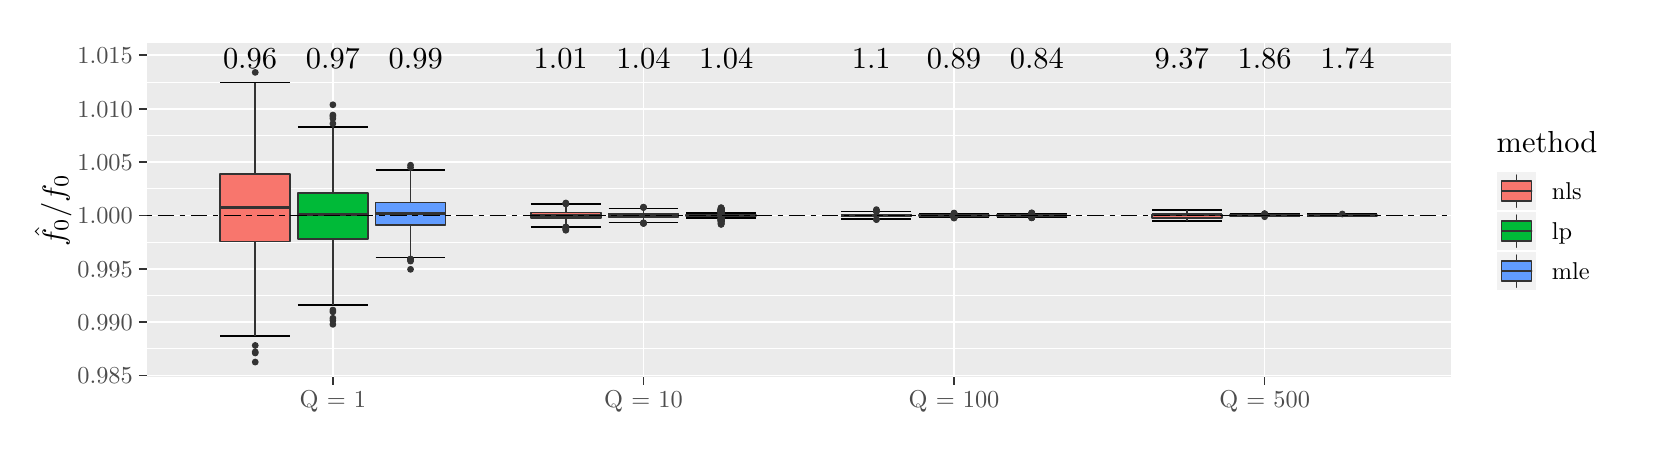
\begin{tikzpicture}[x=1pt,y=1pt]
\definecolor{fillColor}{RGB}{255,255,255}
\path[use as bounding box,fill=fillColor,fill opacity=0.00] (0,0) rectangle (578.16,144.54);
\begin{scope}
\path[clip] (  0.00,  0.00) rectangle (578.16,144.54);
\definecolor{drawColor}{RGB}{255,255,255}
\definecolor{fillColor}{RGB}{255,255,255}

\path[draw=drawColor,line width= 0.6pt,line join=round,line cap=round,fill=fillColor] (  0.00,  0.00) rectangle (578.16,144.54);
\end{scope}
\begin{scope}
\path[clip] ( 42.95, 18.22) rectangle (514.31,139.04);
\definecolor{fillColor}{gray}{0.92}

\path[fill=fillColor] ( 42.95, 18.22) rectangle (514.31,139.04);
\definecolor{drawColor}{RGB}{255,255,255}

\path[draw=drawColor,line width= 0.3pt,line join=round] ( 42.95, 28.49) --
	(514.31, 28.49);

\path[draw=drawColor,line width= 0.3pt,line join=round] ( 42.95, 47.77) --
	(514.31, 47.77);

\path[draw=drawColor,line width= 0.3pt,line join=round] ( 42.95, 67.06) --
	(514.31, 67.06);

\path[draw=drawColor,line width= 0.3pt,line join=round] ( 42.95, 86.34) --
	(514.31, 86.34);

\path[draw=drawColor,line width= 0.3pt,line join=round] ( 42.95,105.63) --
	(514.31,105.63);

\path[draw=drawColor,line width= 0.3pt,line join=round] ( 42.95,124.91) --
	(514.31,124.91);

\path[draw=drawColor,line width= 0.6pt,line join=round] ( 42.95, 18.84) --
	(514.31, 18.84);

\path[draw=drawColor,line width= 0.6pt,line join=round] ( 42.95, 38.13) --
	(514.31, 38.13);

\path[draw=drawColor,line width= 0.6pt,line join=round] ( 42.95, 57.41) --
	(514.31, 57.41);

\path[draw=drawColor,line width= 0.6pt,line join=round] ( 42.95, 76.70) --
	(514.31, 76.70);

\path[draw=drawColor,line width= 0.6pt,line join=round] ( 42.95, 95.99) --
	(514.31, 95.99);

\path[draw=drawColor,line width= 0.6pt,line join=round] ( 42.95,115.27) --
	(514.31,115.27);

\path[draw=drawColor,line width= 0.6pt,line join=round] ( 42.95,134.56) --
	(514.31,134.56);

\path[draw=drawColor,line width= 0.6pt,line join=round] (110.29, 18.22) --
	(110.29,139.04);

\path[draw=drawColor,line width= 0.6pt,line join=round] (222.52, 18.22) --
	(222.52,139.04);

\path[draw=drawColor,line width= 0.6pt,line join=round] (334.74, 18.22) --
	(334.74,139.04);

\path[draw=drawColor,line width= 0.6pt,line join=round] (446.97, 18.22) --
	(446.97,139.04);
\definecolor{drawColor}{RGB}{0,0,0}

\path[draw=drawColor,line width= 0.6pt,line join=round] ( 69.61,124.67) --
	( 94.86,124.67);

\path[draw=drawColor,line width= 0.6pt,line join=round] ( 82.23,124.67) --
	( 82.23, 33.03);

\path[draw=drawColor,line width= 0.6pt,line join=round] ( 69.61, 33.03) --
	( 94.86, 33.03);

\path[draw=drawColor,line width= 0.6pt,line join=round] ( 97.66,108.56) --
	(122.92,108.56);

\path[draw=drawColor,line width= 0.6pt,line join=round] (110.29,108.56) --
	(110.29, 44.37);

\path[draw=drawColor,line width= 0.6pt,line join=round] ( 97.66, 44.37) --
	(122.92, 44.37);

\path[draw=drawColor,line width= 0.6pt,line join=round] (125.72, 93.16) --
	(150.97, 93.16);

\path[draw=drawColor,line width= 0.6pt,line join=round] (138.35, 93.16) --
	(138.35, 61.46);

\path[draw=drawColor,line width= 0.6pt,line join=round] (125.72, 61.46) --
	(150.97, 61.46);

\path[draw=drawColor,line width= 0.6pt,line join=round] (181.83, 80.83) --
	(207.09, 80.83);

\path[draw=drawColor,line width= 0.6pt,line join=round] (194.46, 80.83) --
	(194.46, 72.57);

\path[draw=drawColor,line width= 0.6pt,line join=round] (181.83, 72.57) --
	(207.09, 72.57);

\path[draw=drawColor,line width= 0.6pt,line join=round] (209.89, 79.17) --
	(235.14, 79.17);

\path[draw=drawColor,line width= 0.6pt,line join=round] (222.52, 79.17) --
	(222.52, 74.08);

\path[draw=drawColor,line width= 0.6pt,line join=round] (209.89, 74.08) --
	(235.14, 74.08);

\path[draw=drawColor,line width= 0.6pt,line join=round] (237.95, 77.51) --
	(263.20, 77.51);

\path[draw=drawColor,line width= 0.6pt,line join=round] (250.57, 77.51) --
	(250.57, 75.79);

\path[draw=drawColor,line width= 0.6pt,line join=round] (237.95, 75.79) --
	(263.20, 75.79);

\path[draw=drawColor,line width= 0.6pt,line join=round] (294.06, 78.07) --
	(319.31, 78.07);

\path[draw=drawColor,line width= 0.6pt,line join=round] (306.69, 78.07) --
	(306.69, 75.32);

\path[draw=drawColor,line width= 0.6pt,line join=round] (294.06, 75.32) --
	(319.31, 75.32);

\path[draw=drawColor,line width= 0.6pt,line join=round] (322.12, 77.36) --
	(347.37, 77.36);

\path[draw=drawColor,line width= 0.6pt,line join=round] (334.74, 77.36) --
	(334.74, 76.00);

\path[draw=drawColor,line width= 0.6pt,line join=round] (322.12, 76.00) --
	(347.37, 76.00);

\path[draw=drawColor,line width= 0.6pt,line join=round] (350.18, 77.37) --
	(375.43, 77.37);

\path[draw=drawColor,line width= 0.6pt,line join=round] (362.80, 77.37) --
	(362.80, 76.00);

\path[draw=drawColor,line width= 0.6pt,line join=round] (350.18, 76.00) --
	(375.43, 76.00);

\path[draw=drawColor,line width= 0.6pt,line join=round] (406.29, 78.73) --
	(431.54, 78.73);

\path[draw=drawColor,line width= 0.6pt,line join=round] (418.91, 78.73) --
	(418.91, 74.74);

\path[draw=drawColor,line width= 0.6pt,line join=round] (406.29, 74.74) --
	(431.54, 74.74);

\path[draw=drawColor,line width= 0.6pt,line join=round] (434.35, 77.15) --
	(459.60, 77.15);

\path[draw=drawColor,line width= 0.6pt,line join=round] (446.97, 77.15) --
	(446.97, 76.26);

\path[draw=drawColor,line width= 0.6pt,line join=round] (434.35, 76.26) --
	(459.60, 76.26);

\path[draw=drawColor,line width= 0.6pt,line join=round] (462.40, 77.16) --
	(487.65, 77.16);

\path[draw=drawColor,line width= 0.6pt,line join=round] (475.03, 77.16) --
	(475.03, 76.27);

\path[draw=drawColor,line width= 0.6pt,line join=round] (462.40, 76.27) --
	(487.65, 76.27);
\definecolor{drawColor}{gray}{0.20}
\definecolor{fillColor}{gray}{0.20}

\path[draw=drawColor,line width= 0.4pt,line join=round,line cap=round,fill=fillColor] ( 82.23, 27.38) circle (  1.02);

\path[draw=drawColor,line width= 0.4pt,line join=round,line cap=round,fill=fillColor] ( 82.23, 23.71) circle (  1.02);

\path[draw=drawColor,line width= 0.4pt,line join=round,line cap=round,fill=fillColor] ( 82.23,128.38) circle (  1.02);

\path[draw=drawColor,line width= 0.4pt,line join=round,line cap=round,fill=fillColor] ( 82.23, 29.71) circle (  1.02);

\path[draw=drawColor,line width= 0.4pt,line join=round,line cap=round,fill=fillColor] ( 82.23, 26.99) circle (  1.02);

\path[draw=drawColor,line width= 0.6pt,line join=round] ( 82.23, 91.70) -- ( 82.23,124.67);

\path[draw=drawColor,line width= 0.6pt,line join=round] ( 82.23, 67.31) -- ( 82.23, 33.03);
\definecolor{fillColor}{RGB}{248,118,109}

\path[draw=drawColor,line width= 0.6pt,line join=round,line cap=round,fill=fillColor] ( 69.61, 91.70) --
	( 69.61, 67.31) --
	( 94.86, 67.31) --
	( 94.86, 91.70) --
	( 69.61, 91.70) --
	cycle;

\path[draw=drawColor,line width= 1.1pt,line join=round] ( 69.61, 79.60) -- ( 94.86, 79.60);
\definecolor{fillColor}{gray}{0.20}

\path[draw=drawColor,line width= 0.4pt,line join=round,line cap=round,fill=fillColor] (110.29,112.98) circle (  1.02);

\path[draw=drawColor,line width= 0.4pt,line join=round,line cap=round,fill=fillColor] (110.29, 38.76) circle (  1.02);

\path[draw=drawColor,line width= 0.4pt,line join=round,line cap=round,fill=fillColor] (110.29,112.53) circle (  1.02);

\path[draw=drawColor,line width= 0.4pt,line join=round,line cap=round,fill=fillColor] (110.29,109.87) circle (  1.02);

\path[draw=drawColor,line width= 0.4pt,line join=round,line cap=round,fill=fillColor] (110.29,116.68) circle (  1.02);

\path[draw=drawColor,line width= 0.4pt,line join=round,line cap=round,fill=fillColor] (110.29, 37.34) circle (  1.02);

\path[draw=drawColor,line width= 0.4pt,line join=round,line cap=round,fill=fillColor] (110.29, 42.51) circle (  1.02);

\path[draw=drawColor,line width= 0.4pt,line join=round,line cap=round,fill=fillColor] (110.29,111.73) circle (  1.02);

\path[draw=drawColor,line width= 0.4pt,line join=round,line cap=round,fill=fillColor] (110.29, 39.55) circle (  1.02);

\path[draw=drawColor,line width= 0.4pt,line join=round,line cap=round,fill=fillColor] (110.29, 41.85) circle (  1.02);

\path[draw=drawColor,line width= 0.6pt,line join=round] (110.29, 84.71) -- (110.29,108.56);

\path[draw=drawColor,line width= 0.6pt,line join=round] (110.29, 68.07) -- (110.29, 44.37);
\definecolor{fillColor}{RGB}{0,186,56}

\path[draw=drawColor,line width= 0.6pt,line join=round,line cap=round,fill=fillColor] ( 97.66, 84.71) --
	( 97.66, 68.07) --
	(122.92, 68.07) --
	(122.92, 84.71) --
	( 97.66, 84.71) --
	cycle;

\path[draw=drawColor,line width= 1.1pt,line join=round] ( 97.66, 77.11) -- (122.92, 77.11);
\definecolor{fillColor}{gray}{0.20}

\path[draw=drawColor,line width= 0.4pt,line join=round,line cap=round,fill=fillColor] (138.35, 60.83) circle (  1.02);

\path[draw=drawColor,line width= 0.4pt,line join=round,line cap=round,fill=fillColor] (138.35, 60.81) circle (  1.02);

\path[draw=drawColor,line width= 0.4pt,line join=round,line cap=round,fill=fillColor] (138.35, 57.21) circle (  1.02);

\path[draw=drawColor,line width= 0.4pt,line join=round,line cap=round,fill=fillColor] (138.35, 60.94) circle (  1.02);

\path[draw=drawColor,line width= 0.4pt,line join=round,line cap=round,fill=fillColor] (138.35, 93.99) circle (  1.02);

\path[draw=drawColor,line width= 0.4pt,line join=round,line cap=round,fill=fillColor] (138.35, 94.85) circle (  1.02);

\path[draw=drawColor,line width= 0.4pt,line join=round,line cap=round,fill=fillColor] (138.35, 60.19) circle (  1.02);

\path[draw=drawColor,line width= 0.6pt,line join=round] (138.35, 81.33) -- (138.35, 93.16);

\path[draw=drawColor,line width= 0.6pt,line join=round] (138.35, 73.35) -- (138.35, 61.46);
\definecolor{fillColor}{RGB}{97,156,255}

\path[draw=drawColor,line width= 0.6pt,line join=round,line cap=round,fill=fillColor] (125.72, 81.33) --
	(125.72, 73.35) --
	(150.97, 73.35) --
	(150.97, 81.33) --
	(125.72, 81.33) --
	cycle;

\path[draw=drawColor,line width= 1.1pt,line join=round] (125.72, 77.45) -- (150.97, 77.45);
\definecolor{fillColor}{gray}{0.20}

\path[draw=drawColor,line width= 0.4pt,line join=round,line cap=round,fill=fillColor] (194.46, 71.34) circle (  1.02);

\path[draw=drawColor,line width= 0.4pt,line join=round,line cap=round,fill=fillColor] (194.46, 72.39) circle (  1.02);

\path[draw=drawColor,line width= 0.4pt,line join=round,line cap=round,fill=fillColor] (194.46, 72.40) circle (  1.02);

\path[draw=drawColor,line width= 0.4pt,line join=round,line cap=round,fill=fillColor] (194.46, 71.56) circle (  1.02);

\path[draw=drawColor,line width= 0.4pt,line join=round,line cap=round,fill=fillColor] (194.46, 71.97) circle (  1.02);

\path[draw=drawColor,line width= 0.4pt,line join=round,line cap=round,fill=fillColor] (194.46, 72.45) circle (  1.02);

\path[draw=drawColor,line width= 0.4pt,line join=round,line cap=round,fill=fillColor] (194.46, 80.94) circle (  1.02);

\path[draw=drawColor,line width= 0.4pt,line join=round,line cap=round,fill=fillColor] (194.46, 81.19) circle (  1.02);

\path[draw=drawColor,line width= 0.4pt,line join=round,line cap=round,fill=fillColor] (194.46, 80.86) circle (  1.02);

\path[draw=drawColor,line width= 0.4pt,line join=round,line cap=round,fill=fillColor] (194.46, 72.52) circle (  1.02);

\path[draw=drawColor,line width= 0.4pt,line join=round,line cap=round,fill=fillColor] (194.46, 72.35) circle (  1.02);

\path[draw=drawColor,line width= 0.6pt,line join=round] (194.46, 77.73) -- (194.46, 80.83);

\path[draw=drawColor,line width= 0.6pt,line join=round] (194.46, 75.65) -- (194.46, 72.57);
\definecolor{fillColor}{RGB}{248,118,109}

\path[draw=drawColor,line width= 0.6pt,line join=round,line cap=round,fill=fillColor] (181.83, 77.73) --
	(181.83, 75.65) --
	(207.09, 75.65) --
	(207.09, 77.73) --
	(181.83, 77.73) --
	cycle;

\path[draw=drawColor,line width= 1.1pt,line join=round] (181.83, 76.53) -- (207.09, 76.53);
\definecolor{fillColor}{gray}{0.20}

\path[draw=drawColor,line width= 0.4pt,line join=round,line cap=round,fill=fillColor] (222.52, 73.80) circle (  1.02);

\path[draw=drawColor,line width= 0.4pt,line join=round,line cap=round,fill=fillColor] (222.52, 74.02) circle (  1.02);

\path[draw=drawColor,line width= 0.4pt,line join=round,line cap=round,fill=fillColor] (222.52, 79.57) circle (  1.02);

\path[draw=drawColor,line width= 0.4pt,line join=round,line cap=round,fill=fillColor] (222.52, 79.63) circle (  1.02);

\path[draw=drawColor,line width= 0.4pt,line join=round,line cap=round,fill=fillColor] (222.52, 73.91) circle (  1.02);

\path[draw=drawColor,line width= 0.4pt,line join=round,line cap=round,fill=fillColor] (222.52, 73.82) circle (  1.02);

\path[draw=drawColor,line width= 0.4pt,line join=round,line cap=round,fill=fillColor] (222.52, 79.63) circle (  1.02);

\path[draw=drawColor,line width= 0.6pt,line join=round] (222.52, 77.34) -- (222.52, 79.17);

\path[draw=drawColor,line width= 0.6pt,line join=round] (222.52, 76.02) -- (222.52, 74.08);
\definecolor{fillColor}{RGB}{0,186,56}

\path[draw=drawColor,line width= 0.6pt,line join=round,line cap=round,fill=fillColor] (209.89, 77.34) --
	(209.89, 76.02) --
	(235.14, 76.02) --
	(235.14, 77.34) --
	(209.89, 77.34) --
	cycle;

\path[draw=drawColor,line width= 1.1pt,line join=round] (209.89, 76.68) -- (235.14, 76.68);
\definecolor{fillColor}{gray}{0.20}

\path[draw=drawColor,line width= 0.4pt,line join=round,line cap=round,fill=fillColor] (250.57, 77.89) circle (  1.02);

\path[draw=drawColor,line width= 0.4pt,line join=round,line cap=round,fill=fillColor] (250.57, 75.45) circle (  1.02);

\path[draw=drawColor,line width= 0.4pt,line join=round,line cap=round,fill=fillColor] (250.57, 77.80) circle (  1.02);

\path[draw=drawColor,line width= 0.4pt,line join=round,line cap=round,fill=fillColor] (250.57, 78.38) circle (  1.02);

\path[draw=drawColor,line width= 0.4pt,line join=round,line cap=round,fill=fillColor] (250.57, 78.67) circle (  1.02);

\path[draw=drawColor,line width= 0.4pt,line join=round,line cap=round,fill=fillColor] (250.57, 77.74) circle (  1.02);

\path[draw=drawColor,line width= 0.4pt,line join=round,line cap=round,fill=fillColor] (250.57, 78.49) circle (  1.02);

\path[draw=drawColor,line width= 0.4pt,line join=round,line cap=round,fill=fillColor] (250.57, 75.35) circle (  1.02);

\path[draw=drawColor,line width= 0.4pt,line join=round,line cap=round,fill=fillColor] (250.57, 78.21) circle (  1.02);

\path[draw=drawColor,line width= 0.4pt,line join=round,line cap=round,fill=fillColor] (250.57, 77.53) circle (  1.02);

\path[draw=drawColor,line width= 0.4pt,line join=round,line cap=round,fill=fillColor] (250.57, 73.79) circle (  1.02);

\path[draw=drawColor,line width= 0.4pt,line join=round,line cap=round,fill=fillColor] (250.57, 78.25) circle (  1.02);

\path[draw=drawColor,line width= 0.4pt,line join=round,line cap=round,fill=fillColor] (250.57, 77.92) circle (  1.02);

\path[draw=drawColor,line width= 0.4pt,line join=round,line cap=round,fill=fillColor] (250.57, 78.99) circle (  1.02);

\path[draw=drawColor,line width= 0.4pt,line join=round,line cap=round,fill=fillColor] (250.57, 78.54) circle (  1.02);

\path[draw=drawColor,line width= 0.4pt,line join=round,line cap=round,fill=fillColor] (250.57, 73.90) circle (  1.02);

\path[draw=drawColor,line width= 0.4pt,line join=round,line cap=round,fill=fillColor] (250.57, 78.54) circle (  1.02);

\path[draw=drawColor,line width= 0.4pt,line join=round,line cap=round,fill=fillColor] (250.57, 78.31) circle (  1.02);

\path[draw=drawColor,line width= 0.4pt,line join=round,line cap=round,fill=fillColor] (250.57, 78.07) circle (  1.02);

\path[draw=drawColor,line width= 0.4pt,line join=round,line cap=round,fill=fillColor] (250.57, 78.13) circle (  1.02);

\path[draw=drawColor,line width= 0.4pt,line join=round,line cap=round,fill=fillColor] (250.57, 78.41) circle (  1.02);

\path[draw=drawColor,line width= 0.4pt,line join=round,line cap=round,fill=fillColor] (250.57, 75.69) circle (  1.02);

\path[draw=drawColor,line width= 0.4pt,line join=round,line cap=round,fill=fillColor] (250.57, 74.87) circle (  1.02);

\path[draw=drawColor,line width= 0.4pt,line join=round,line cap=round,fill=fillColor] (250.57, 78.71) circle (  1.02);

\path[draw=drawColor,line width= 0.4pt,line join=round,line cap=round,fill=fillColor] (250.57, 74.37) circle (  1.02);

\path[draw=drawColor,line width= 0.4pt,line join=round,line cap=round,fill=fillColor] (250.57, 77.56) circle (  1.02);

\path[draw=drawColor,line width= 0.4pt,line join=round,line cap=round,fill=fillColor] (250.57, 77.61) circle (  1.02);

\path[draw=drawColor,line width= 0.4pt,line join=round,line cap=round,fill=fillColor] (250.57, 78.44) circle (  1.02);

\path[draw=drawColor,line width= 0.4pt,line join=round,line cap=round,fill=fillColor] (250.57, 78.83) circle (  1.02);

\path[draw=drawColor,line width= 0.4pt,line join=round,line cap=round,fill=fillColor] (250.57, 75.38) circle (  1.02);

\path[draw=drawColor,line width= 0.4pt,line join=round,line cap=round,fill=fillColor] (250.57, 77.91) circle (  1.02);

\path[draw=drawColor,line width= 0.4pt,line join=round,line cap=round,fill=fillColor] (250.57, 78.06) circle (  1.02);

\path[draw=drawColor,line width= 0.4pt,line join=round,line cap=round,fill=fillColor] (250.57, 74.71) circle (  1.02);

\path[draw=drawColor,line width= 0.4pt,line join=round,line cap=round,fill=fillColor] (250.57, 78.86) circle (  1.02);

\path[draw=drawColor,line width= 0.4pt,line join=round,line cap=round,fill=fillColor] (250.57, 79.32) circle (  1.02);

\path[draw=drawColor,line width= 0.4pt,line join=round,line cap=round,fill=fillColor] (250.57, 79.41) circle (  1.02);

\path[draw=drawColor,line width= 0.4pt,line join=round,line cap=round,fill=fillColor] (250.57, 75.15) circle (  1.02);

\path[draw=drawColor,line width= 0.4pt,line join=round,line cap=round,fill=fillColor] (250.57, 77.84) circle (  1.02);

\path[draw=drawColor,line width= 0.4pt,line join=round,line cap=round,fill=fillColor] (250.57, 78.81) circle (  1.02);

\path[draw=drawColor,line width= 0.4pt,line join=round,line cap=round,fill=fillColor] (250.57, 75.69) circle (  1.02);

\path[draw=drawColor,line width= 0.4pt,line join=round,line cap=round,fill=fillColor] (250.57, 74.73) circle (  1.02);

\path[draw=drawColor,line width= 0.4pt,line join=round,line cap=round,fill=fillColor] (250.57, 77.56) circle (  1.02);

\path[draw=drawColor,line width= 0.4pt,line join=round,line cap=round,fill=fillColor] (250.57, 78.14) circle (  1.02);

\path[draw=drawColor,line width= 0.4pt,line join=round,line cap=round,fill=fillColor] (250.57, 79.19) circle (  1.02);

\path[draw=drawColor,line width= 0.4pt,line join=round,line cap=round,fill=fillColor] (250.57, 77.82) circle (  1.02);

\path[draw=drawColor,line width= 0.4pt,line join=round,line cap=round,fill=fillColor] (250.57, 74.92) circle (  1.02);

\path[draw=drawColor,line width= 0.4pt,line join=round,line cap=round,fill=fillColor] (250.57, 77.65) circle (  1.02);

\path[draw=drawColor,line width= 0.4pt,line join=round,line cap=round,fill=fillColor] (250.57, 75.70) circle (  1.02);

\path[draw=drawColor,line width= 0.4pt,line join=round,line cap=round,fill=fillColor] (250.57, 78.04) circle (  1.02);

\path[draw=drawColor,line width= 0.4pt,line join=round,line cap=round,fill=fillColor] (250.57, 77.94) circle (  1.02);

\path[draw=drawColor,line width= 0.4pt,line join=round,line cap=round,fill=fillColor] (250.57, 75.51) circle (  1.02);

\path[draw=drawColor,line width= 0.4pt,line join=round,line cap=round,fill=fillColor] (250.57, 78.28) circle (  1.02);

\path[draw=drawColor,line width= 0.4pt,line join=round,line cap=round,fill=fillColor] (250.57, 75.06) circle (  1.02);

\path[draw=drawColor,line width= 0.4pt,line join=round,line cap=round,fill=fillColor] (250.57, 77.72) circle (  1.02);

\path[draw=drawColor,line width= 0.4pt,line join=round,line cap=round,fill=fillColor] (250.57, 75.71) circle (  1.02);

\path[draw=drawColor,line width= 0.4pt,line join=round,line cap=round,fill=fillColor] (250.57, 77.88) circle (  1.02);

\path[draw=drawColor,line width= 0.4pt,line join=round,line cap=round,fill=fillColor] (250.57, 78.89) circle (  1.02);

\path[draw=drawColor,line width= 0.4pt,line join=round,line cap=round,fill=fillColor] (250.57, 78.56) circle (  1.02);

\path[draw=drawColor,line width= 0.4pt,line join=round,line cap=round,fill=fillColor] (250.57, 79.10) circle (  1.02);

\path[draw=drawColor,line width= 0.4pt,line join=round,line cap=round,fill=fillColor] (250.57, 74.80) circle (  1.02);

\path[draw=drawColor,line width= 0.4pt,line join=round,line cap=round,fill=fillColor] (250.57, 73.50) circle (  1.02);

\path[draw=drawColor,line width= 0.4pt,line join=round,line cap=round,fill=fillColor] (250.57, 78.17) circle (  1.02);

\path[draw=drawColor,line width= 0.4pt,line join=round,line cap=round,fill=fillColor] (250.57, 77.86) circle (  1.02);

\path[draw=drawColor,line width= 0.4pt,line join=round,line cap=round,fill=fillColor] (250.57, 78.34) circle (  1.02);

\path[draw=drawColor,line width= 0.4pt,line join=round,line cap=round,fill=fillColor] (250.57, 78.66) circle (  1.02);

\path[draw=drawColor,line width= 0.4pt,line join=round,line cap=round,fill=fillColor] (250.57, 78.01) circle (  1.02);

\path[draw=drawColor,line width= 0.4pt,line join=round,line cap=round,fill=fillColor] (250.57, 77.72) circle (  1.02);

\path[draw=drawColor,line width= 0.4pt,line join=round,line cap=round,fill=fillColor] (250.57, 78.07) circle (  1.02);

\path[draw=drawColor,line width= 0.4pt,line join=round,line cap=round,fill=fillColor] (250.57, 74.77) circle (  1.02);

\path[draw=drawColor,line width= 0.4pt,line join=round,line cap=round,fill=fillColor] (250.57, 74.04) circle (  1.02);

\path[draw=drawColor,line width= 0.4pt,line join=round,line cap=round,fill=fillColor] (250.57, 74.66) circle (  1.02);

\path[draw=drawColor,line width= 0.4pt,line join=round,line cap=round,fill=fillColor] (250.57, 78.26) circle (  1.02);

\path[draw=drawColor,line width= 0.4pt,line join=round,line cap=round,fill=fillColor] (250.57, 78.12) circle (  1.02);

\path[draw=drawColor,line width= 0.4pt,line join=round,line cap=round,fill=fillColor] (250.57, 77.67) circle (  1.02);

\path[draw=drawColor,line width= 0.4pt,line join=round,line cap=round,fill=fillColor] (250.57, 78.84) circle (  1.02);

\path[draw=drawColor,line width= 0.4pt,line join=round,line cap=round,fill=fillColor] (250.57, 74.88) circle (  1.02);

\path[draw=drawColor,line width= 0.4pt,line join=round,line cap=round,fill=fillColor] (250.57, 78.62) circle (  1.02);

\path[draw=drawColor,line width= 0.4pt,line join=round,line cap=round,fill=fillColor] (250.57, 77.86) circle (  1.02);

\path[draw=drawColor,line width= 0.4pt,line join=round,line cap=round,fill=fillColor] (250.57, 77.62) circle (  1.02);

\path[draw=drawColor,line width= 0.4pt,line join=round,line cap=round,fill=fillColor] (250.57, 78.13) circle (  1.02);

\path[draw=drawColor,line width= 0.4pt,line join=round,line cap=round,fill=fillColor] (250.57, 78.33) circle (  1.02);

\path[draw=drawColor,line width= 0.4pt,line join=round,line cap=round,fill=fillColor] (250.57, 77.85) circle (  1.02);

\path[draw=drawColor,line width= 0.4pt,line join=round,line cap=round,fill=fillColor] (250.57, 75.58) circle (  1.02);

\path[draw=drawColor,line width= 0.4pt,line join=round,line cap=round,fill=fillColor] (250.57, 77.78) circle (  1.02);

\path[draw=drawColor,line width= 0.4pt,line join=round,line cap=round,fill=fillColor] (250.57, 75.34) circle (  1.02);

\path[draw=drawColor,line width= 0.4pt,line join=round,line cap=round,fill=fillColor] (250.57, 77.56) circle (  1.02);

\path[draw=drawColor,line width= 0.4pt,line join=round,line cap=round,fill=fillColor] (250.57, 78.40) circle (  1.02);

\path[draw=drawColor,line width= 0.4pt,line join=round,line cap=round,fill=fillColor] (250.57, 75.21) circle (  1.02);

\path[draw=drawColor,line width= 0.4pt,line join=round,line cap=round,fill=fillColor] (250.57, 74.39) circle (  1.02);

\path[draw=drawColor,line width= 0.4pt,line join=round,line cap=round,fill=fillColor] (250.57, 77.71) circle (  1.02);

\path[draw=drawColor,line width= 0.4pt,line join=round,line cap=round,fill=fillColor] (250.57, 78.10) circle (  1.02);

\path[draw=drawColor,line width= 0.4pt,line join=round,line cap=round,fill=fillColor] (250.57, 78.20) circle (  1.02);

\path[draw=drawColor,line width= 0.4pt,line join=round,line cap=round,fill=fillColor] (250.57, 78.03) circle (  1.02);

\path[draw=drawColor,line width= 0.4pt,line join=round,line cap=round,fill=fillColor] (250.57, 74.50) circle (  1.02);

\path[draw=drawColor,line width= 0.4pt,line join=round,line cap=round,fill=fillColor] (250.57, 78.71) circle (  1.02);

\path[draw=drawColor,line width= 0.4pt,line join=round,line cap=round,fill=fillColor] (250.57, 77.69) circle (  1.02);

\path[draw=drawColor,line width= 0.4pt,line join=round,line cap=round,fill=fillColor] (250.57, 79.12) circle (  1.02);

\path[draw=drawColor,line width= 0.4pt,line join=round,line cap=round,fill=fillColor] (250.57, 78.73) circle (  1.02);

\path[draw=drawColor,line width= 0.4pt,line join=round,line cap=round,fill=fillColor] (250.57, 75.30) circle (  1.02);

\path[draw=drawColor,line width= 0.4pt,line join=round,line cap=round,fill=fillColor] (250.57, 77.66) circle (  1.02);

\path[draw=drawColor,line width= 0.4pt,line join=round,line cap=round,fill=fillColor] (250.57, 77.94) circle (  1.02);

\path[draw=drawColor,line width= 0.4pt,line join=round,line cap=round,fill=fillColor] (250.57, 78.60) circle (  1.02);

\path[draw=drawColor,line width= 0.4pt,line join=round,line cap=round,fill=fillColor] (250.57, 78.42) circle (  1.02);

\path[draw=drawColor,line width= 0.4pt,line join=round,line cap=round,fill=fillColor] (250.57, 77.56) circle (  1.02);

\path[draw=drawColor,line width= 0.4pt,line join=round,line cap=round,fill=fillColor] (250.57, 75.31) circle (  1.02);

\path[draw=drawColor,line width= 0.4pt,line join=round,line cap=round,fill=fillColor] (250.57, 78.62) circle (  1.02);

\path[draw=drawColor,line width= 0.4pt,line join=round,line cap=round,fill=fillColor] (250.57, 78.25) circle (  1.02);

\path[draw=drawColor,line width= 0.4pt,line join=round,line cap=round,fill=fillColor] (250.57, 75.66) circle (  1.02);

\path[draw=drawColor,line width= 0.4pt,line join=round,line cap=round,fill=fillColor] (250.57, 77.58) circle (  1.02);

\path[draw=drawColor,line width= 0.4pt,line join=round,line cap=round,fill=fillColor] (250.57, 77.70) circle (  1.02);

\path[draw=drawColor,line width= 0.4pt,line join=round,line cap=round,fill=fillColor] (250.57, 77.69) circle (  1.02);

\path[draw=drawColor,line width= 0.4pt,line join=round,line cap=round,fill=fillColor] (250.57, 78.44) circle (  1.02);

\path[draw=drawColor,line width= 0.4pt,line join=round,line cap=round,fill=fillColor] (250.57, 75.11) circle (  1.02);

\path[draw=drawColor,line width= 0.4pt,line join=round,line cap=round,fill=fillColor] (250.57, 73.63) circle (  1.02);

\path[draw=drawColor,line width= 0.4pt,line join=round,line cap=round,fill=fillColor] (250.57, 77.65) circle (  1.02);

\path[draw=drawColor,line width= 0.4pt,line join=round,line cap=round,fill=fillColor] (250.57, 78.52) circle (  1.02);

\path[draw=drawColor,line width= 0.4pt,line join=round,line cap=round,fill=fillColor] (250.57, 77.64) circle (  1.02);

\path[draw=drawColor,line width= 0.4pt,line join=round,line cap=round,fill=fillColor] (250.57, 77.77) circle (  1.02);

\path[draw=drawColor,line width= 0.4pt,line join=round,line cap=round,fill=fillColor] (250.57, 78.25) circle (  1.02);

\path[draw=drawColor,line width= 0.4pt,line join=round,line cap=round,fill=fillColor] (250.57, 77.88) circle (  1.02);

\path[draw=drawColor,line width= 0.4pt,line join=round,line cap=round,fill=fillColor] (250.57, 78.21) circle (  1.02);

\path[draw=drawColor,line width= 0.4pt,line join=round,line cap=round,fill=fillColor] (250.57, 77.68) circle (  1.02);

\path[draw=drawColor,line width= 0.4pt,line join=round,line cap=round,fill=fillColor] (250.57, 77.52) circle (  1.02);

\path[draw=drawColor,line width= 0.4pt,line join=round,line cap=round,fill=fillColor] (250.57, 78.49) circle (  1.02);

\path[draw=drawColor,line width= 0.4pt,line join=round,line cap=round,fill=fillColor] (250.57, 75.66) circle (  1.02);

\path[draw=drawColor,line width= 0.4pt,line join=round,line cap=round,fill=fillColor] (250.57, 75.54) circle (  1.02);

\path[draw=drawColor,line width= 0.4pt,line join=round,line cap=round,fill=fillColor] (250.57, 78.62) circle (  1.02);

\path[draw=drawColor,line width= 0.4pt,line join=round,line cap=round,fill=fillColor] (250.57, 78.07) circle (  1.02);

\path[draw=drawColor,line width= 0.4pt,line join=round,line cap=round,fill=fillColor] (250.57, 77.77) circle (  1.02);

\path[draw=drawColor,line width= 0.4pt,line join=round,line cap=round,fill=fillColor] (250.57, 73.49) circle (  1.02);

\path[draw=drawColor,line width= 0.4pt,line join=round,line cap=round,fill=fillColor] (250.57, 78.43) circle (  1.02);

\path[draw=drawColor,line width= 0.4pt,line join=round,line cap=round,fill=fillColor] (250.57, 78.13) circle (  1.02);

\path[draw=drawColor,line width= 0.4pt,line join=round,line cap=round,fill=fillColor] (250.57, 77.92) circle (  1.02);

\path[draw=drawColor,line width= 0.4pt,line join=round,line cap=round,fill=fillColor] (250.57, 75.76) circle (  1.02);

\path[draw=drawColor,line width= 0.4pt,line join=round,line cap=round,fill=fillColor] (250.57, 78.61) circle (  1.02);

\path[draw=drawColor,line width= 0.4pt,line join=round,line cap=round,fill=fillColor] (250.57, 77.63) circle (  1.02);

\path[draw=drawColor,line width= 0.4pt,line join=round,line cap=round,fill=fillColor] (250.57, 77.67) circle (  1.02);

\path[draw=drawColor,line width= 0.4pt,line join=round,line cap=round,fill=fillColor] (250.57, 75.03) circle (  1.02);

\path[draw=drawColor,line width= 0.4pt,line join=round,line cap=round,fill=fillColor] (250.57, 78.29) circle (  1.02);

\path[draw=drawColor,line width= 0.4pt,line join=round,line cap=round,fill=fillColor] (250.57, 75.76) circle (  1.02);

\path[draw=drawColor,line width= 0.4pt,line join=round,line cap=round,fill=fillColor] (250.57, 77.62) circle (  1.02);

\path[draw=drawColor,line width= 0.4pt,line join=round,line cap=round,fill=fillColor] (250.57, 78.20) circle (  1.02);

\path[draw=drawColor,line width= 0.4pt,line join=round,line cap=round,fill=fillColor] (250.57, 77.95) circle (  1.02);

\path[draw=drawColor,line width= 0.4pt,line join=round,line cap=round,fill=fillColor] (250.57, 77.96) circle (  1.02);

\path[draw=drawColor,line width= 0.4pt,line join=round,line cap=round,fill=fillColor] (250.57, 75.20) circle (  1.02);

\path[draw=drawColor,line width= 0.4pt,line join=round,line cap=round,fill=fillColor] (250.57, 75.51) circle (  1.02);

\path[draw=drawColor,line width= 0.4pt,line join=round,line cap=round,fill=fillColor] (250.57, 79.24) circle (  1.02);

\path[draw=drawColor,line width= 0.4pt,line join=round,line cap=round,fill=fillColor] (250.57, 77.69) circle (  1.02);

\path[draw=drawColor,line width= 0.4pt,line join=round,line cap=round,fill=fillColor] (250.57, 78.63) circle (  1.02);

\path[draw=drawColor,line width= 0.4pt,line join=round,line cap=round,fill=fillColor] (250.57, 77.60) circle (  1.02);

\path[draw=drawColor,line width= 0.4pt,line join=round,line cap=round,fill=fillColor] (250.57, 74.92) circle (  1.02);

\path[draw=drawColor,line width= 0.4pt,line join=round,line cap=round,fill=fillColor] (250.57, 77.78) circle (  1.02);

\path[draw=drawColor,line width= 0.4pt,line join=round,line cap=round,fill=fillColor] (250.57, 77.59) circle (  1.02);

\path[draw=drawColor,line width= 0.4pt,line join=round,line cap=round,fill=fillColor] (250.57, 75.73) circle (  1.02);

\path[draw=drawColor,line width= 0.4pt,line join=round,line cap=round,fill=fillColor] (250.57, 77.92) circle (  1.02);

\path[draw=drawColor,line width= 0.4pt,line join=round,line cap=round,fill=fillColor] (250.57, 79.49) circle (  1.02);

\path[draw=drawColor,line width= 0.6pt,line join=round] (250.57, 76.86) -- (250.57, 77.51);

\path[draw=drawColor,line width= 0.6pt,line join=round] (250.57, 76.42) -- (250.57, 75.79);
\definecolor{fillColor}{RGB}{97,156,255}

\path[draw=drawColor,line width= 0.6pt,line join=round,line cap=round,fill=fillColor] (237.95, 76.86) --
	(237.95, 76.42) --
	(263.20, 76.42) --
	(263.20, 76.86) --
	(237.95, 76.86) --
	cycle;

\path[draw=drawColor,line width= 1.1pt,line join=round] (237.95, 76.61) -- (263.20, 76.61);
\definecolor{fillColor}{gray}{0.20}

\path[draw=drawColor,line width= 0.4pt,line join=round,line cap=round,fill=fillColor] (306.69, 78.80) circle (  1.02);

\path[draw=drawColor,line width= 0.4pt,line join=round,line cap=round,fill=fillColor] (306.69, 75.28) circle (  1.02);

\path[draw=drawColor,line width= 0.4pt,line join=round,line cap=round,fill=fillColor] (306.69, 78.35) circle (  1.02);

\path[draw=drawColor,line width= 0.4pt,line join=round,line cap=round,fill=fillColor] (306.69, 78.15) circle (  1.02);

\path[draw=drawColor,line width= 0.4pt,line join=round,line cap=round,fill=fillColor] (306.69, 75.18) circle (  1.02);

\path[draw=drawColor,line width= 0.4pt,line join=round,line cap=round,fill=fillColor] (306.69, 78.13) circle (  1.02);

\path[draw=drawColor,line width= 0.6pt,line join=round] (306.69, 77.06) -- (306.69, 78.07);

\path[draw=drawColor,line width= 0.6pt,line join=round] (306.69, 76.36) -- (306.69, 75.32);
\definecolor{fillColor}{RGB}{248,118,109}

\path[draw=drawColor,line width= 0.6pt,line join=round,line cap=round,fill=fillColor] (294.06, 77.06) --
	(294.06, 76.36) --
	(319.31, 76.36) --
	(319.31, 77.06) --
	(294.06, 77.06) --
	cycle;

\path[draw=drawColor,line width= 1.1pt,line join=round] (294.06, 76.72) -- (319.31, 76.72);
\definecolor{fillColor}{gray}{0.20}

\path[draw=drawColor,line width= 0.4pt,line join=round,line cap=round,fill=fillColor] (334.74, 75.94) circle (  1.02);

\path[draw=drawColor,line width= 0.4pt,line join=round,line cap=round,fill=fillColor] (334.74, 75.77) circle (  1.02);

\path[draw=drawColor,line width= 0.4pt,line join=round,line cap=round,fill=fillColor] (334.74, 75.97) circle (  1.02);

\path[draw=drawColor,line width= 0.4pt,line join=round,line cap=round,fill=fillColor] (334.74, 75.94) circle (  1.02);

\path[draw=drawColor,line width= 0.4pt,line join=round,line cap=round,fill=fillColor] (334.74, 75.94) circle (  1.02);

\path[draw=drawColor,line width= 0.4pt,line join=round,line cap=round,fill=fillColor] (334.74, 77.41) circle (  1.02);

\path[draw=drawColor,line width= 0.4pt,line join=round,line cap=round,fill=fillColor] (334.74, 75.83) circle (  1.02);

\path[draw=drawColor,line width= 0.4pt,line join=round,line cap=round,fill=fillColor] (334.74, 77.55) circle (  1.02);

\path[draw=drawColor,line width= 0.4pt,line join=round,line cap=round,fill=fillColor] (334.74, 75.88) circle (  1.02);

\path[draw=drawColor,line width= 0.4pt,line join=round,line cap=round,fill=fillColor] (334.74, 77.41) circle (  1.02);

\path[draw=drawColor,line width= 0.4pt,line join=round,line cap=round,fill=fillColor] (334.74, 77.40) circle (  1.02);

\path[draw=drawColor,line width= 0.6pt,line join=round] (334.74, 76.86) -- (334.74, 77.36);

\path[draw=drawColor,line width= 0.6pt,line join=round] (334.74, 76.51) -- (334.74, 76.00);
\definecolor{fillColor}{RGB}{0,186,56}

\path[draw=drawColor,line width= 0.6pt,line join=round,line cap=round,fill=fillColor] (322.12, 76.86) --
	(322.12, 76.51) --
	(347.37, 76.51) --
	(347.37, 76.86) --
	(322.12, 76.86) --
	cycle;

\path[draw=drawColor,line width= 1.1pt,line join=round] (322.12, 76.68) -- (347.37, 76.68);
\definecolor{fillColor}{gray}{0.20}

\path[draw=drawColor,line width= 0.4pt,line join=round,line cap=round,fill=fillColor] (362.80, 75.85) circle (  1.02);

\path[draw=drawColor,line width= 0.4pt,line join=round,line cap=round,fill=fillColor] (362.80, 75.85) circle (  1.02);

\path[draw=drawColor,line width= 0.4pt,line join=round,line cap=round,fill=fillColor] (362.80, 75.96) circle (  1.02);

\path[draw=drawColor,line width= 0.4pt,line join=round,line cap=round,fill=fillColor] (362.80, 75.94) circle (  1.02);

\path[draw=drawColor,line width= 0.4pt,line join=round,line cap=round,fill=fillColor] (362.80, 77.47) circle (  1.02);

\path[draw=drawColor,line width= 0.4pt,line join=round,line cap=round,fill=fillColor] (362.80, 77.41) circle (  1.02);

\path[draw=drawColor,line width= 0.4pt,line join=round,line cap=round,fill=fillColor] (362.80, 75.86) circle (  1.02);

\path[draw=drawColor,line width= 0.4pt,line join=round,line cap=round,fill=fillColor] (362.80, 75.96) circle (  1.02);

\path[draw=drawColor,line width= 0.4pt,line join=round,line cap=round,fill=fillColor] (362.80, 77.41) circle (  1.02);

\path[draw=drawColor,line width= 0.4pt,line join=round,line cap=round,fill=fillColor] (362.80, 77.63) circle (  1.02);

\path[draw=drawColor,line width= 0.4pt,line join=round,line cap=round,fill=fillColor] (362.80, 75.98) circle (  1.02);

\path[draw=drawColor,line width= 0.4pt,line join=round,line cap=round,fill=fillColor] (362.80, 77.55) circle (  1.02);

\path[draw=drawColor,line width= 0.6pt,line join=round] (362.80, 76.86) -- (362.80, 77.37);

\path[draw=drawColor,line width= 0.6pt,line join=round] (362.80, 76.51) -- (362.80, 76.00);
\definecolor{fillColor}{RGB}{97,156,255}

\path[draw=drawColor,line width= 0.6pt,line join=round,line cap=round,fill=fillColor] (350.18, 76.86) --
	(350.18, 76.51) --
	(375.43, 76.51) --
	(375.43, 76.86) --
	(350.18, 76.86) --
	cycle;

\path[draw=drawColor,line width= 1.1pt,line join=round] (350.18, 76.69) -- (375.43, 76.69);

\path[draw=drawColor,line width= 0.6pt,line join=round] (418.91, 77.06) -- (418.91, 78.73);

\path[draw=drawColor,line width= 0.6pt,line join=round] (418.91, 75.87) -- (418.91, 74.74);
\definecolor{fillColor}{RGB}{248,118,109}

\path[draw=drawColor,line width= 0.6pt,line join=round,line cap=round,fill=fillColor] (406.29, 77.06) --
	(406.29, 75.87) --
	(431.54, 75.87) --
	(431.54, 77.06) --
	(406.29, 77.06) --
	cycle;

\path[draw=drawColor,line width= 1.1pt,line join=round] (406.29, 76.93) -- (431.54, 76.93);
\definecolor{fillColor}{gray}{0.20}

\path[draw=drawColor,line width= 0.4pt,line join=round,line cap=round,fill=fillColor] (446.97, 76.23) circle (  1.02);

\path[draw=drawColor,line width= 0.4pt,line join=round,line cap=round,fill=fillColor] (446.97, 77.18) circle (  1.02);

\path[draw=drawColor,line width= 0.4pt,line join=round,line cap=round,fill=fillColor] (446.97, 77.29) circle (  1.02);

\path[draw=drawColor,line width= 0.4pt,line join=round,line cap=round,fill=fillColor] (446.97, 77.18) circle (  1.02);

\path[draw=drawColor,line width= 0.4pt,line join=round,line cap=round,fill=fillColor] (446.97, 77.19) circle (  1.02);

\path[draw=drawColor,line width= 0.4pt,line join=round,line cap=round,fill=fillColor] (446.97, 77.28) circle (  1.02);

\path[draw=drawColor,line width= 0.6pt,line join=round] (446.97, 76.82) -- (446.97, 77.15);

\path[draw=drawColor,line width= 0.6pt,line join=round] (446.97, 76.60) -- (446.97, 76.26);
\definecolor{fillColor}{RGB}{0,186,56}

\path[draw=drawColor,line width= 0.6pt,line join=round,line cap=round,fill=fillColor] (434.35, 76.82) --
	(434.35, 76.60) --
	(459.60, 76.60) --
	(459.60, 76.82) --
	(434.35, 76.82) --
	cycle;

\path[draw=drawColor,line width= 1.1pt,line join=round] (434.35, 76.72) -- (459.60, 76.72);
\definecolor{fillColor}{gray}{0.20}

\path[draw=drawColor,line width= 0.4pt,line join=round,line cap=round,fill=fillColor] (475.03, 77.21) circle (  1.02);

\path[draw=drawColor,line width= 0.6pt,line join=round] (475.03, 76.83) -- (475.03, 77.16);

\path[draw=drawColor,line width= 0.6pt,line join=round] (475.03, 76.60) -- (475.03, 76.27);
\definecolor{fillColor}{RGB}{97,156,255}

\path[draw=drawColor,line width= 0.6pt,line join=round,line cap=round,fill=fillColor] (462.40, 76.83) --
	(462.40, 76.60) --
	(487.65, 76.60) --
	(487.65, 76.83) --
	(462.40, 76.83) --
	cycle;

\path[draw=drawColor,line width= 1.1pt,line join=round] (462.40, 76.71) -- (487.65, 76.71);
\definecolor{drawColor}{RGB}{0,0,0}

\path[draw=drawColor,line width= 0.6pt,dash pattern=on 2pt off 2pt on 6pt off 2pt ,line join=round] ( 42.95, 76.70) -- (514.31, 76.70);

\node[text=drawColor,anchor=base,inner sep=0pt, outer sep=0pt, scale=  1.10] at (140.22,129.75) {0.99};

\node[text=drawColor,anchor=base,inner sep=0pt, outer sep=0pt, scale=  1.10] at (110.29,129.75) {0.97};

\node[text=drawColor,anchor=base,inner sep=0pt, outer sep=0pt, scale=  1.10] at ( 80.36,129.75) {0.96};

\node[text=drawColor,anchor=base,inner sep=0pt, outer sep=0pt, scale=  1.10] at (252.44,129.75) {1.04};

\node[text=drawColor,anchor=base,inner sep=0pt, outer sep=0pt, scale=  1.10] at (222.52,129.75) {1.04};

\node[text=drawColor,anchor=base,inner sep=0pt, outer sep=0pt, scale=  1.10] at (192.59,129.75) {1.01};

\node[text=drawColor,anchor=base,inner sep=0pt, outer sep=0pt, scale=  1.10] at (364.67,129.75) {0.84};

\node[text=drawColor,anchor=base,inner sep=0pt, outer sep=0pt, scale=  1.10] at (334.74,129.75) {0.89};

\node[text=drawColor,anchor=base,inner sep=0pt, outer sep=0pt, scale=  1.10] at (304.82,129.75) {1.1};

\node[text=drawColor,anchor=base,inner sep=0pt, outer sep=0pt, scale=  1.10] at (476.90,129.75) {1.74};

\node[text=drawColor,anchor=base,inner sep=0pt, outer sep=0pt, scale=  1.10] at (446.97,129.75) {1.86};

\node[text=drawColor,anchor=base,inner sep=0pt, outer sep=0pt, scale=  1.10] at (417.04,129.75) {9.37};
\end{scope}
\begin{scope}
\path[clip] (  0.00,  0.00) rectangle (578.16,144.54);
\definecolor{drawColor}{gray}{0.30}

\node[text=drawColor,anchor=base east,inner sep=0pt, outer sep=0pt, scale=  0.88] at ( 38.00, 15.81) {0.985};

\node[text=drawColor,anchor=base east,inner sep=0pt, outer sep=0pt, scale=  0.88] at ( 38.00, 35.10) {0.990};

\node[text=drawColor,anchor=base east,inner sep=0pt, outer sep=0pt, scale=  0.88] at ( 38.00, 54.38) {0.995};

\node[text=drawColor,anchor=base east,inner sep=0pt, outer sep=0pt, scale=  0.88] at ( 38.00, 73.67) {1.000};

\node[text=drawColor,anchor=base east,inner sep=0pt, outer sep=0pt, scale=  0.88] at ( 38.00, 92.95) {1.005};

\node[text=drawColor,anchor=base east,inner sep=0pt, outer sep=0pt, scale=  0.88] at ( 38.00,112.24) {1.010};

\node[text=drawColor,anchor=base east,inner sep=0pt, outer sep=0pt, scale=  0.88] at ( 38.00,131.53) {1.015};
\end{scope}
\begin{scope}
\path[clip] (  0.00,  0.00) rectangle (578.16,144.54);
\definecolor{drawColor}{gray}{0.20}

\path[draw=drawColor,line width= 0.6pt,line join=round] ( 40.20, 18.84) --
	( 42.95, 18.84);

\path[draw=drawColor,line width= 0.6pt,line join=round] ( 40.20, 38.13) --
	( 42.95, 38.13);

\path[draw=drawColor,line width= 0.6pt,line join=round] ( 40.20, 57.41) --
	( 42.95, 57.41);

\path[draw=drawColor,line width= 0.6pt,line join=round] ( 40.20, 76.70) --
	( 42.95, 76.70);

\path[draw=drawColor,line width= 0.6pt,line join=round] ( 40.20, 95.99) --
	( 42.95, 95.99);

\path[draw=drawColor,line width= 0.6pt,line join=round] ( 40.20,115.27) --
	( 42.95,115.27);

\path[draw=drawColor,line width= 0.6pt,line join=round] ( 40.20,134.56) --
	( 42.95,134.56);
\end{scope}
\begin{scope}
\path[clip] (  0.00,  0.00) rectangle (578.16,144.54);
\definecolor{drawColor}{gray}{0.20}

\path[draw=drawColor,line width= 0.6pt,line join=round] (110.29, 15.47) --
	(110.29, 18.22);

\path[draw=drawColor,line width= 0.6pt,line join=round] (222.52, 15.47) --
	(222.52, 18.22);

\path[draw=drawColor,line width= 0.6pt,line join=round] (334.74, 15.47) --
	(334.74, 18.22);

\path[draw=drawColor,line width= 0.6pt,line join=round] (446.97, 15.47) --
	(446.97, 18.22);
\end{scope}
\begin{scope}
\path[clip] (  0.00,  0.00) rectangle (578.16,144.54);
\definecolor{drawColor}{gray}{0.30}

\node[text=drawColor,anchor=base,inner sep=0pt, outer sep=0pt, scale=  0.88] at (110.29,  7.21) {Q = 1};

\node[text=drawColor,anchor=base,inner sep=0pt, outer sep=0pt, scale=  0.88] at (222.52,  7.21) {Q = 10};

\node[text=drawColor,anchor=base,inner sep=0pt, outer sep=0pt, scale=  0.88] at (334.74,  7.21) {Q = 100};

\node[text=drawColor,anchor=base,inner sep=0pt, outer sep=0pt, scale=  0.88] at (446.97,  7.21) {Q = 500};
\end{scope}
\begin{scope}
\path[clip] (  0.00,  0.00) rectangle (578.16,144.54);
\definecolor{drawColor}{RGB}{0,0,0}

\node[text=drawColor,rotate= 90.00,anchor=base,inner sep=0pt, outer sep=0pt, scale=  1.10] at ( 13.08, 78.63) {$\hat{f_0}/f_0$};
\end{scope}
\begin{scope}
\path[clip] (  0.00,  0.00) rectangle (578.16,144.54);
\definecolor{fillColor}{RGB}{255,255,255}

\path[fill=fillColor] (525.31, 43.84) rectangle (572.66,113.42);
\end{scope}
\begin{scope}
\path[clip] (  0.00,  0.00) rectangle (578.16,144.54);
\definecolor{drawColor}{RGB}{0,0,0}

\node[text=drawColor,anchor=base west,inner sep=0pt, outer sep=0pt, scale=  1.10] at (530.81, 99.27) {method};
\end{scope}
\begin{scope}
\path[clip] (  0.00,  0.00) rectangle (578.16,144.54);
\definecolor{drawColor}{RGB}{255,255,255}
\definecolor{fillColor}{gray}{0.95}

\path[draw=drawColor,line width= 0.6pt,line join=round,line cap=round,fill=fillColor] (530.81, 78.25) rectangle (545.26, 92.70);
\end{scope}
\begin{scope}
\path[clip] (  0.00,  0.00) rectangle (578.16,144.54);
\definecolor{drawColor}{gray}{0.20}

\path[draw=drawColor,line width= 0.6pt,line join=round,line cap=round] (538.03, 79.70) --
	(538.03, 81.86);

\path[draw=drawColor,line width= 0.6pt,line join=round,line cap=round] (538.03, 89.09) --
	(538.03, 91.26);
\definecolor{fillColor}{RGB}{248,118,109}

\path[draw=drawColor,line width= 0.6pt,line join=round,line cap=round,fill=fillColor] (532.61, 81.86) rectangle (543.45, 89.09);

\path[draw=drawColor,line width= 0.6pt,line join=round,line cap=round] (532.61, 85.48) --
	(543.45, 85.48);
\end{scope}
\begin{scope}
\path[clip] (  0.00,  0.00) rectangle (578.16,144.54);
\definecolor{drawColor}{RGB}{255,255,255}
\definecolor{fillColor}{gray}{0.95}

\path[draw=drawColor,line width= 0.6pt,line join=round,line cap=round,fill=fillColor] (530.81, 63.80) rectangle (545.26, 78.25);
\end{scope}
\begin{scope}
\path[clip] (  0.00,  0.00) rectangle (578.16,144.54);
\definecolor{drawColor}{gray}{0.20}

\path[draw=drawColor,line width= 0.6pt,line join=round,line cap=round] (538.03, 65.24) --
	(538.03, 67.41);

\path[draw=drawColor,line width= 0.6pt,line join=round,line cap=round] (538.03, 74.64) --
	(538.03, 76.81);
\definecolor{fillColor}{RGB}{0,186,56}

\path[draw=drawColor,line width= 0.6pt,line join=round,line cap=round,fill=fillColor] (532.61, 67.41) rectangle (543.45, 74.64);

\path[draw=drawColor,line width= 0.6pt,line join=round,line cap=round] (532.61, 71.02) --
	(543.45, 71.02);
\end{scope}
\begin{scope}
\path[clip] (  0.00,  0.00) rectangle (578.16,144.54);
\definecolor{drawColor}{RGB}{255,255,255}
\definecolor{fillColor}{gray}{0.95}

\path[draw=drawColor,line width= 0.6pt,line join=round,line cap=round,fill=fillColor] (530.81, 49.34) rectangle (545.26, 63.80);
\end{scope}
\begin{scope}
\path[clip] (  0.00,  0.00) rectangle (578.16,144.54);
\definecolor{drawColor}{gray}{0.20}

\path[draw=drawColor,line width= 0.6pt,line join=round,line cap=round] (538.03, 50.79) --
	(538.03, 52.96);

\path[draw=drawColor,line width= 0.6pt,line join=round,line cap=round] (538.03, 60.18) --
	(538.03, 62.35);
\definecolor{fillColor}{RGB}{97,156,255}

\path[draw=drawColor,line width= 0.6pt,line join=round,line cap=round,fill=fillColor] (532.61, 52.96) rectangle (543.45, 60.18);

\path[draw=drawColor,line width= 0.6pt,line join=round,line cap=round] (532.61, 56.57) --
	(543.45, 56.57);
\end{scope}
\begin{scope}
\path[clip] (  0.00,  0.00) rectangle (578.16,144.54);
\definecolor{drawColor}{RGB}{0,0,0}

\node[text=drawColor,anchor=base west,inner sep=0pt, outer sep=0pt, scale=  0.88] at (550.76, 82.45) {nls};
\end{scope}
\begin{scope}
\path[clip] (  0.00,  0.00) rectangle (578.16,144.54);
\definecolor{drawColor}{RGB}{0,0,0}

\node[text=drawColor,anchor=base west,inner sep=0pt, outer sep=0pt, scale=  0.88] at (550.76, 67.99) {lp};
\end{scope}
\begin{scope}
\path[clip] (  0.00,  0.00) rectangle (578.16,144.54);
\definecolor{drawColor}{RGB}{0,0,0}

\node[text=drawColor,anchor=base west,inner sep=0pt, outer sep=0pt, scale=  0.88] at (550.76, 53.54) {mle};
\end{scope}
\end{tikzpicture}
}
  \end{subfigure}
  \caption{Comparison of NLS, LP and MLE preliminary estimators (prior to noise removal) in the noise-contaminated environment. Numbers indicate MSE ratios of the corresponding estimators to their own performance at baseline.}
\end{figure}

\begin{figure}
  \begin{subfigure}
    \centering
    \resizebox{1.1\linewidth}{!}{% Created by tikzDevice version 0.12.3 on 2019-09-30 11:20:19
% !TEX encoding = UTF-8 Unicode
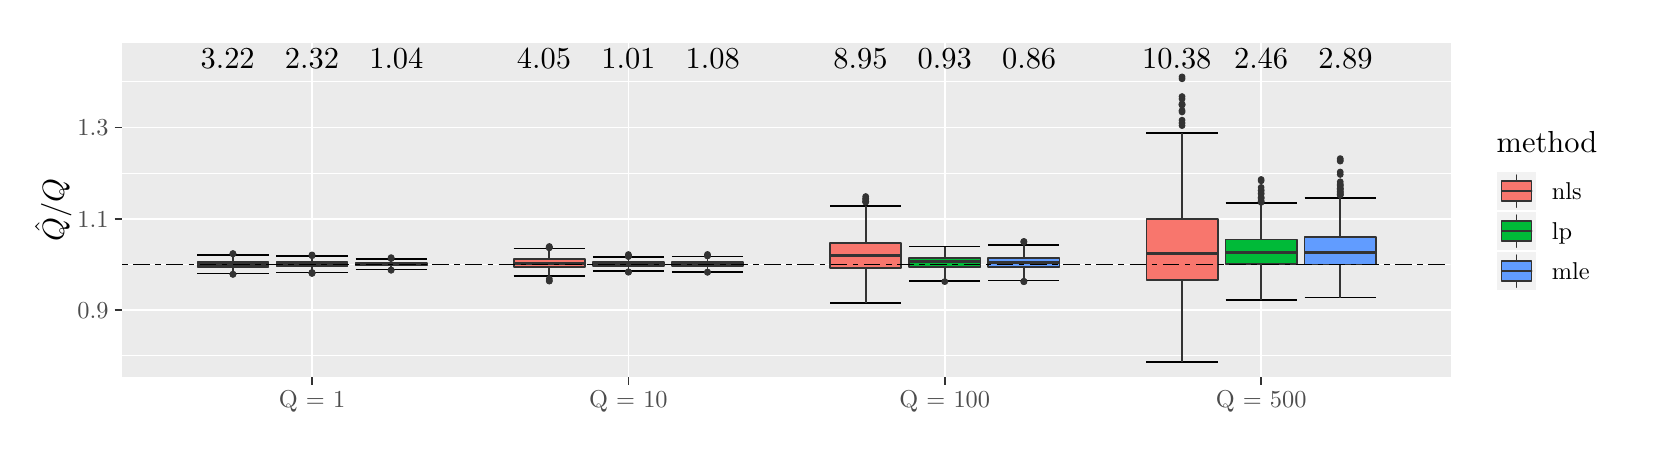
\begin{tikzpicture}[x=1pt,y=1pt]
\definecolor{fillColor}{RGB}{255,255,255}
\path[use as bounding box,fill=fillColor,fill opacity=0.00] (0,0) rectangle (578.16,144.54);
\begin{scope}
\path[clip] (  0.00,  0.00) rectangle (578.16,144.54);
\definecolor{drawColor}{RGB}{255,255,255}
\definecolor{fillColor}{RGB}{255,255,255}

\path[draw=drawColor,line width= 0.6pt,line join=round,line cap=round,fill=fillColor] (  0.00,  0.00) rectangle (578.16,144.54);
\end{scope}
\begin{scope}
\path[clip] ( 34.16, 18.22) rectangle (514.31,139.04);
\definecolor{fillColor}{gray}{0.92}

\path[fill=fillColor] ( 34.16, 18.22) rectangle (514.31,139.04);
\definecolor{drawColor}{RGB}{255,255,255}

\path[draw=drawColor,line width= 0.3pt,line join=round] ( 34.16, 26.06) --
	(514.31, 26.06);

\path[draw=drawColor,line width= 0.3pt,line join=round] ( 34.16, 59.02) --
	(514.31, 59.02);

\path[draw=drawColor,line width= 0.3pt,line join=round] ( 34.16, 91.98) --
	(514.31, 91.98);

\path[draw=drawColor,line width= 0.3pt,line join=round] ( 34.16,124.94) --
	(514.31,124.94);

\path[draw=drawColor,line width= 0.6pt,line join=round] ( 34.16, 42.54) --
	(514.31, 42.54);

\path[draw=drawColor,line width= 0.6pt,line join=round] ( 34.16, 75.50) --
	(514.31, 75.50);

\path[draw=drawColor,line width= 0.6pt,line join=round] ( 34.16,108.46) --
	(514.31,108.46);

\path[draw=drawColor,line width= 0.6pt,line join=round] (102.75, 18.22) --
	(102.75,139.04);

\path[draw=drawColor,line width= 0.6pt,line join=round] (217.07, 18.22) --
	(217.07,139.04);

\path[draw=drawColor,line width= 0.6pt,line join=round] (331.39, 18.22) --
	(331.39,139.04);

\path[draw=drawColor,line width= 0.6pt,line join=round] (445.71, 18.22) --
	(445.71,139.04);
\definecolor{drawColor}{RGB}{0,0,0}

\path[draw=drawColor,line width= 0.6pt,line join=round] ( 61.31, 62.51) --
	( 87.03, 62.51);

\path[draw=drawColor,line width= 0.6pt,line join=round] ( 74.17, 62.51) --
	( 74.17, 55.75);

\path[draw=drawColor,line width= 0.6pt,line join=round] ( 61.31, 55.75) --
	( 87.03, 55.75);

\path[draw=drawColor,line width= 0.6pt,line join=round] ( 89.89, 61.97) --
	(115.61, 61.97);

\path[draw=drawColor,line width= 0.6pt,line join=round] (102.75, 61.97) --
	(102.75, 56.12);

\path[draw=drawColor,line width= 0.6pt,line join=round] ( 89.89, 56.12) --
	(115.61, 56.12);

\path[draw=drawColor,line width= 0.6pt,line join=round] (118.47, 60.94) --
	(144.19, 60.94);

\path[draw=drawColor,line width= 0.6pt,line join=round] (131.33, 60.94) --
	(131.33, 57.10);

\path[draw=drawColor,line width= 0.6pt,line join=round] (118.47, 57.10) --
	(144.19, 57.10);

\path[draw=drawColor,line width= 0.6pt,line join=round] (175.63, 64.79) --
	(201.35, 64.79);

\path[draw=drawColor,line width= 0.6pt,line join=round] (188.49, 64.79) --
	(188.49, 54.70);

\path[draw=drawColor,line width= 0.6pt,line join=round] (175.63, 54.70) --
	(201.35, 54.70);

\path[draw=drawColor,line width= 0.6pt,line join=round] (204.21, 61.71) --
	(229.93, 61.71);

\path[draw=drawColor,line width= 0.6pt,line join=round] (217.07, 61.71) --
	(217.07, 56.61);

\path[draw=drawColor,line width= 0.6pt,line join=round] (204.21, 56.61) --
	(229.93, 56.61);

\path[draw=drawColor,line width= 0.6pt,line join=round] (232.79, 61.90) --
	(258.51, 61.90);

\path[draw=drawColor,line width= 0.6pt,line join=round] (245.65, 61.90) --
	(245.65, 56.37);

\path[draw=drawColor,line width= 0.6pt,line join=round] (232.79, 56.37) --
	(258.51, 56.37);

\path[draw=drawColor,line width= 0.6pt,line join=round] (289.95, 80.09) --
	(315.67, 80.09);

\path[draw=drawColor,line width= 0.6pt,line join=round] (302.81, 80.09) --
	(302.81, 45.07);

\path[draw=drawColor,line width= 0.6pt,line join=round] (289.95, 45.07) --
	(315.67, 45.07);

\path[draw=drawColor,line width= 0.6pt,line join=round] (318.53, 65.42) --
	(344.25, 65.42);

\path[draw=drawColor,line width= 0.6pt,line join=round] (331.39, 65.42) --
	(331.39, 52.97);

\path[draw=drawColor,line width= 0.6pt,line join=round] (318.53, 52.97) --
	(344.25, 52.97);

\path[draw=drawColor,line width= 0.6pt,line join=round] (347.11, 65.96) --
	(372.83, 65.96);

\path[draw=drawColor,line width= 0.6pt,line join=round] (359.97, 65.96) --
	(359.97, 53.24);

\path[draw=drawColor,line width= 0.6pt,line join=round] (347.11, 53.24) --
	(372.83, 53.24);

\path[draw=drawColor,line width= 0.6pt,line join=round] (404.27,106.49) --
	(430.00,106.49);

\path[draw=drawColor,line width= 0.6pt,line join=round] (417.13,106.49) --
	(417.13, 23.71);

\path[draw=drawColor,line width= 0.6pt,line join=round] (404.27, 23.71) --
	(430.00, 23.71);

\path[draw=drawColor,line width= 0.6pt,line join=round] (432.85, 81.29) --
	(458.58, 81.29);

\path[draw=drawColor,line width= 0.6pt,line join=round] (445.71, 81.29) --
	(445.71, 46.19);

\path[draw=drawColor,line width= 0.6pt,line join=round] (432.85, 46.19) --
	(458.58, 46.19);

\path[draw=drawColor,line width= 0.6pt,line join=round] (461.43, 82.95) --
	(487.16, 82.95);

\path[draw=drawColor,line width= 0.6pt,line join=round] (474.29, 82.95) --
	(474.29, 46.99);

\path[draw=drawColor,line width= 0.6pt,line join=round] (461.43, 46.99) --
	(487.16, 46.99);
\definecolor{drawColor}{gray}{0.20}
\definecolor{fillColor}{gray}{0.20}

\path[draw=drawColor,line width= 0.4pt,line join=round,line cap=round,fill=fillColor] ( 74.17, 62.92) circle (  1.02);

\path[draw=drawColor,line width= 0.4pt,line join=round,line cap=round,fill=fillColor] ( 74.17, 55.43) circle (  1.02);

\path[draw=drawColor,line width= 0.4pt,line join=round,line cap=round,fill=fillColor] ( 74.17, 55.42) circle (  1.02);

\path[draw=drawColor,line width= 0.4pt,line join=round,line cap=round,fill=fillColor] ( 74.17, 62.80) circle (  1.02);

\path[draw=drawColor,line width= 0.6pt,line join=round] ( 74.17, 59.88) -- ( 74.17, 62.51);

\path[draw=drawColor,line width= 0.6pt,line join=round] ( 74.17, 58.12) -- ( 74.17, 55.75);
\definecolor{fillColor}{RGB}{248,118,109}

\path[draw=drawColor,line width= 0.6pt,line join=round,line cap=round,fill=fillColor] ( 61.31, 59.88) --
	( 61.31, 58.12) --
	( 87.03, 58.12) --
	( 87.03, 59.88) --
	( 61.31, 59.88) --
	cycle;

\path[draw=drawColor,line width= 1.1pt,line join=round] ( 61.31, 58.96) -- ( 87.03, 58.96);
\definecolor{fillColor}{gray}{0.20}

\path[draw=drawColor,line width= 0.4pt,line join=round,line cap=round,fill=fillColor] (102.75, 56.06) circle (  1.02);

\path[draw=drawColor,line width= 0.4pt,line join=round,line cap=round,fill=fillColor] (102.75, 55.96) circle (  1.02);

\path[draw=drawColor,line width= 0.4pt,line join=round,line cap=round,fill=fillColor] (102.75, 62.12) circle (  1.02);

\path[draw=drawColor,line width= 0.4pt,line join=round,line cap=round,fill=fillColor] (102.75, 62.43) circle (  1.02);

\path[draw=drawColor,line width= 0.4pt,line join=round,line cap=round,fill=fillColor] (102.75, 55.72) circle (  1.02);

\path[draw=drawColor,line width= 0.4pt,line join=round,line cap=round,fill=fillColor] (102.75, 55.92) circle (  1.02);

\path[draw=drawColor,line width= 0.6pt,line join=round] (102.75, 59.76) -- (102.75, 61.97);

\path[draw=drawColor,line width= 0.6pt,line join=round] (102.75, 58.29) -- (102.75, 56.12);
\definecolor{fillColor}{RGB}{0,186,56}

\path[draw=drawColor,line width= 0.6pt,line join=round,line cap=round,fill=fillColor] ( 89.89, 59.76) --
	( 89.89, 58.29) --
	(115.61, 58.29) --
	(115.61, 59.76) --
	( 89.89, 59.76) --
	cycle;

\path[draw=drawColor,line width= 1.1pt,line join=round] ( 89.89, 59.02) -- (115.61, 59.02);
\definecolor{fillColor}{gray}{0.20}

\path[draw=drawColor,line width= 0.4pt,line join=round,line cap=round,fill=fillColor] (131.33, 56.97) circle (  1.02);

\path[draw=drawColor,line width= 0.4pt,line join=round,line cap=round,fill=fillColor] (131.33, 61.45) circle (  1.02);

\path[draw=drawColor,line width= 0.4pt,line join=round,line cap=round,fill=fillColor] (131.33, 61.13) circle (  1.02);

\path[draw=drawColor,line width= 0.4pt,line join=round,line cap=round,fill=fillColor] (131.33, 61.17) circle (  1.02);

\path[draw=drawColor,line width= 0.4pt,line join=round,line cap=round,fill=fillColor] (131.33, 56.90) circle (  1.02);

\path[draw=drawColor,line width= 0.6pt,line join=round] (131.33, 59.52) -- (131.33, 60.94);

\path[draw=drawColor,line width= 0.6pt,line join=round] (131.33, 58.54) -- (131.33, 57.10);
\definecolor{fillColor}{RGB}{97,156,255}

\path[draw=drawColor,line width= 0.6pt,line join=round,line cap=round,fill=fillColor] (118.47, 59.52) --
	(118.47, 58.54) --
	(144.19, 58.54) --
	(144.19, 59.52) --
	(118.47, 59.52) --
	cycle;

\path[draw=drawColor,line width= 1.1pt,line join=round] (118.47, 59.02) -- (144.19, 59.02);
\definecolor{fillColor}{gray}{0.20}

\path[draw=drawColor,line width= 0.4pt,line join=round,line cap=round,fill=fillColor] (188.49, 52.98) circle (  1.02);

\path[draw=drawColor,line width= 0.4pt,line join=round,line cap=round,fill=fillColor] (188.49, 65.06) circle (  1.02);

\path[draw=drawColor,line width= 0.4pt,line join=round,line cap=round,fill=fillColor] (188.49, 65.18) circle (  1.02);

\path[draw=drawColor,line width= 0.4pt,line join=round,line cap=round,fill=fillColor] (188.49, 53.04) circle (  1.02);

\path[draw=drawColor,line width= 0.4pt,line join=round,line cap=round,fill=fillColor] (188.49, 53.80) circle (  1.02);

\path[draw=drawColor,line width= 0.4pt,line join=round,line cap=round,fill=fillColor] (188.49, 65.47) circle (  1.02);

\path[draw=drawColor,line width= 0.4pt,line join=round,line cap=round,fill=fillColor] (188.49, 65.02) circle (  1.02);

\path[draw=drawColor,line width= 0.6pt,line join=round] (188.49, 60.84) -- (188.49, 64.79);

\path[draw=drawColor,line width= 0.6pt,line join=round] (188.49, 58.14) -- (188.49, 54.70);
\definecolor{fillColor}{RGB}{248,118,109}

\path[draw=drawColor,line width= 0.6pt,line join=round,line cap=round,fill=fillColor] (175.63, 60.84) --
	(175.63, 58.14) --
	(201.35, 58.14) --
	(201.35, 60.84) --
	(175.63, 60.84) --
	cycle;

\path[draw=drawColor,line width= 1.1pt,line join=round] (175.63, 59.47) -- (201.35, 59.47);
\definecolor{fillColor}{gray}{0.20}

\path[draw=drawColor,line width= 0.4pt,line join=round,line cap=round,fill=fillColor] (217.07, 56.30) circle (  1.02);

\path[draw=drawColor,line width= 0.4pt,line join=round,line cap=round,fill=fillColor] (217.07, 62.03) circle (  1.02);

\path[draw=drawColor,line width= 0.4pt,line join=round,line cap=round,fill=fillColor] (217.07, 56.20) circle (  1.02);

\path[draw=drawColor,line width= 0.4pt,line join=round,line cap=round,fill=fillColor] (217.07, 62.07) circle (  1.02);

\path[draw=drawColor,line width= 0.4pt,line join=round,line cap=round,fill=fillColor] (217.07, 56.24) circle (  1.02);

\path[draw=drawColor,line width= 0.4pt,line join=round,line cap=round,fill=fillColor] (217.07, 62.00) circle (  1.02);

\path[draw=drawColor,line width= 0.4pt,line join=round,line cap=round,fill=fillColor] (217.07, 62.56) circle (  1.02);

\path[draw=drawColor,line width= 0.4pt,line join=round,line cap=round,fill=fillColor] (217.07, 61.85) circle (  1.02);

\path[draw=drawColor,line width= 0.4pt,line join=round,line cap=round,fill=fillColor] (217.07, 61.98) circle (  1.02);

\path[draw=drawColor,line width= 0.4pt,line join=round,line cap=round,fill=fillColor] (217.07, 62.08) circle (  1.02);

\path[draw=drawColor,line width= 0.6pt,line join=round] (217.07, 59.78) -- (217.07, 61.71);

\path[draw=drawColor,line width= 0.6pt,line join=round] (217.07, 58.45) -- (217.07, 56.61);
\definecolor{fillColor}{RGB}{0,186,56}

\path[draw=drawColor,line width= 0.6pt,line join=round,line cap=round,fill=fillColor] (204.21, 59.78) --
	(204.21, 58.45) --
	(229.93, 58.45) --
	(229.93, 59.78) --
	(204.21, 59.78) --
	cycle;

\path[draw=drawColor,line width= 1.1pt,line join=round] (204.21, 59.11) -- (229.93, 59.11);
\definecolor{fillColor}{gray}{0.20}

\path[draw=drawColor,line width= 0.4pt,line join=round,line cap=round,fill=fillColor] (245.65, 56.23) circle (  1.02);

\path[draw=drawColor,line width= 0.4pt,line join=round,line cap=round,fill=fillColor] (245.65, 56.15) circle (  1.02);

\path[draw=drawColor,line width= 0.4pt,line join=round,line cap=round,fill=fillColor] (245.65, 62.11) circle (  1.02);

\path[draw=drawColor,line width= 0.4pt,line join=round,line cap=round,fill=fillColor] (245.65, 62.59) circle (  1.02);

\path[draw=drawColor,line width= 0.4pt,line join=round,line cap=round,fill=fillColor] (245.65, 62.18) circle (  1.02);

\path[draw=drawColor,line width= 0.4pt,line join=round,line cap=round,fill=fillColor] (245.65, 62.12) circle (  1.02);

\path[draw=drawColor,line width= 0.6pt,line join=round] (245.65, 59.81) -- (245.65, 61.90);

\path[draw=drawColor,line width= 0.6pt,line join=round] (245.65, 58.41) -- (245.65, 56.37);
\definecolor{fillColor}{RGB}{97,156,255}

\path[draw=drawColor,line width= 0.6pt,line join=round,line cap=round,fill=fillColor] (232.79, 59.81) --
	(232.79, 58.41) --
	(258.51, 58.41) --
	(258.51, 59.81) --
	(232.79, 59.81) --
	cycle;

\path[draw=drawColor,line width= 1.1pt,line join=round] (232.79, 59.10) -- (258.51, 59.10);
\definecolor{fillColor}{gray}{0.20}

\path[draw=drawColor,line width= 0.4pt,line join=round,line cap=round,fill=fillColor] (302.81, 81.48) circle (  1.02);

\path[draw=drawColor,line width= 0.4pt,line join=round,line cap=round,fill=fillColor] (302.81, 83.52) circle (  1.02);

\path[draw=drawColor,line width= 0.4pt,line join=round,line cap=round,fill=fillColor] (302.81, 82.78) circle (  1.02);

\path[draw=drawColor,line width= 0.4pt,line join=round,line cap=round,fill=fillColor] (302.81, 81.74) circle (  1.02);

\path[draw=drawColor,line width= 0.4pt,line join=round,line cap=round,fill=fillColor] (302.81, 81.76) circle (  1.02);

\path[draw=drawColor,line width= 0.4pt,line join=round,line cap=round,fill=fillColor] (302.81, 82.57) circle (  1.02);

\path[draw=drawColor,line width= 0.6pt,line join=round] (302.81, 66.80) -- (302.81, 80.09);

\path[draw=drawColor,line width= 0.6pt,line join=round] (302.81, 57.80) -- (302.81, 45.07);
\definecolor{fillColor}{RGB}{248,118,109}

\path[draw=drawColor,line width= 0.6pt,line join=round,line cap=round,fill=fillColor] (289.95, 66.80) --
	(289.95, 57.80) --
	(315.67, 57.80) --
	(315.67, 66.80) --
	(289.95, 66.80) --
	cycle;

\path[draw=drawColor,line width= 1.1pt,line join=round] (289.95, 62.21) -- (315.67, 62.21);
\definecolor{fillColor}{gray}{0.20}

\path[draw=drawColor,line width= 0.4pt,line join=round,line cap=round,fill=fillColor] (331.39, 52.78) circle (  1.02);

\path[draw=drawColor,line width= 0.6pt,line join=round] (331.39, 61.40) -- (331.39, 65.42);

\path[draw=drawColor,line width= 0.6pt,line join=round] (331.39, 58.00) -- (331.39, 52.97);
\definecolor{fillColor}{RGB}{0,186,56}

\path[draw=drawColor,line width= 0.6pt,line join=round,line cap=round,fill=fillColor] (318.53, 61.40) --
	(318.53, 58.00) --
	(344.25, 58.00) --
	(344.25, 61.40) --
	(318.53, 61.40) --
	cycle;

\path[draw=drawColor,line width= 1.1pt,line join=round] (318.53, 59.89) -- (344.25, 59.89);
\definecolor{fillColor}{gray}{0.20}

\path[draw=drawColor,line width= 0.4pt,line join=round,line cap=round,fill=fillColor] (359.97, 67.10) circle (  1.02);

\path[draw=drawColor,line width= 0.4pt,line join=round,line cap=round,fill=fillColor] (359.97, 52.74) circle (  1.02);

\path[draw=drawColor,line width= 0.4pt,line join=round,line cap=round,fill=fillColor] (359.97, 52.85) circle (  1.02);

\path[draw=drawColor,line width= 0.4pt,line join=round,line cap=round,fill=fillColor] (359.97, 52.87) circle (  1.02);

\path[draw=drawColor,line width= 0.4pt,line join=round,line cap=round,fill=fillColor] (359.97, 67.25) circle (  1.02);

\path[draw=drawColor,line width= 0.4pt,line join=round,line cap=round,fill=fillColor] (359.97, 67.26) circle (  1.02);

\path[draw=drawColor,line width= 0.6pt,line join=round] (359.97, 61.21) -- (359.97, 65.96);

\path[draw=drawColor,line width= 0.6pt,line join=round] (359.97, 58.00) -- (359.97, 53.24);
\definecolor{fillColor}{RGB}{97,156,255}

\path[draw=drawColor,line width= 0.6pt,line join=round,line cap=round,fill=fillColor] (347.11, 61.21) --
	(347.11, 58.00) --
	(372.83, 58.00) --
	(372.83, 61.21) --
	(347.11, 61.21) --
	cycle;

\path[draw=drawColor,line width= 1.1pt,line join=round] (347.11, 59.60) -- (372.83, 59.60);
\definecolor{fillColor}{gray}{0.20}

\path[draw=drawColor,line width= 0.4pt,line join=round,line cap=round,fill=fillColor] (417.13,119.65) circle (  1.02);

\path[draw=drawColor,line width= 0.4pt,line join=round,line cap=round,fill=fillColor] (417.13,114.08) circle (  1.02);

\path[draw=drawColor,line width= 0.4pt,line join=round,line cap=round,fill=fillColor] (417.13,110.09) circle (  1.02);

\path[draw=drawColor,line width= 0.4pt,line join=round,line cap=round,fill=fillColor] (417.13,126.07) circle (  1.02);

\path[draw=drawColor,line width= 0.4pt,line join=round,line cap=round,fill=fillColor] (417.13,118.81) circle (  1.02);

\path[draw=drawColor,line width= 0.4pt,line join=round,line cap=round,fill=fillColor] (417.13,116.59) circle (  1.02);

\path[draw=drawColor,line width= 0.4pt,line join=round,line cap=round,fill=fillColor] (417.13,109.16) circle (  1.02);

\path[draw=drawColor,line width= 0.4pt,line join=round,line cap=round,fill=fillColor] (417.13,117.02) circle (  1.02);

\path[draw=drawColor,line width= 0.4pt,line join=round,line cap=round,fill=fillColor] (417.13,111.11) circle (  1.02);

\path[draw=drawColor,line width= 0.4pt,line join=round,line cap=round,fill=fillColor] (417.13,116.72) circle (  1.02);

\path[draw=drawColor,line width= 0.4pt,line join=round,line cap=round,fill=fillColor] (417.13,114.61) circle (  1.02);

\path[draw=drawColor,line width= 0.4pt,line join=round,line cap=round,fill=fillColor] (417.13,126.77) circle (  1.02);

\path[draw=drawColor,line width= 0.6pt,line join=round] (417.13, 75.44) -- (417.13,106.49);

\path[draw=drawColor,line width= 0.6pt,line join=round] (417.13, 53.38) -- (417.13, 23.71);
\definecolor{fillColor}{RGB}{248,118,109}

\path[draw=drawColor,line width= 0.6pt,line join=round,line cap=round,fill=fillColor] (404.27, 75.44) --
	(404.27, 53.38) --
	(430.00, 53.38) --
	(430.00, 75.44) --
	(404.27, 75.44) --
	cycle;

\path[draw=drawColor,line width= 1.1pt,line join=round] (404.27, 62.80) -- (430.00, 62.80);
\definecolor{fillColor}{gray}{0.20}

\path[draw=drawColor,line width= 0.4pt,line join=round,line cap=round,fill=fillColor] (445.71, 84.71) circle (  1.02);

\path[draw=drawColor,line width= 0.4pt,line join=round,line cap=round,fill=fillColor] (445.71, 83.23) circle (  1.02);

\path[draw=drawColor,line width= 0.4pt,line join=round,line cap=round,fill=fillColor] (445.71, 86.82) circle (  1.02);

\path[draw=drawColor,line width= 0.4pt,line join=round,line cap=round,fill=fillColor] (445.71, 81.42) circle (  1.02);

\path[draw=drawColor,line width= 0.4pt,line join=round,line cap=round,fill=fillColor] (445.71, 81.83) circle (  1.02);

\path[draw=drawColor,line width= 0.4pt,line join=round,line cap=round,fill=fillColor] (445.71, 83.08) circle (  1.02);

\path[draw=drawColor,line width= 0.4pt,line join=round,line cap=round,fill=fillColor] (445.71, 82.77) circle (  1.02);

\path[draw=drawColor,line width= 0.4pt,line join=round,line cap=round,fill=fillColor] (445.71, 89.68) circle (  1.02);

\path[draw=drawColor,line width= 0.4pt,line join=round,line cap=round,fill=fillColor] (445.71, 85.80) circle (  1.02);

\path[draw=drawColor,line width= 0.4pt,line join=round,line cap=round,fill=fillColor] (445.71, 84.46) circle (  1.02);

\path[draw=drawColor,line width= 0.4pt,line join=round,line cap=round,fill=fillColor] (445.71, 89.21) circle (  1.02);

\path[draw=drawColor,line width= 0.4pt,line join=round,line cap=round,fill=fillColor] (445.71, 81.77) circle (  1.02);

\path[draw=drawColor,line width= 0.4pt,line join=round,line cap=round,fill=fillColor] (445.71, 85.64) circle (  1.02);

\path[draw=drawColor,line width= 0.6pt,line join=round] (445.71, 68.02) -- (445.71, 81.29);

\path[draw=drawColor,line width= 0.6pt,line join=round] (445.71, 59.17) -- (445.71, 46.19);
\definecolor{fillColor}{RGB}{0,186,56}

\path[draw=drawColor,line width= 0.6pt,line join=round,line cap=round,fill=fillColor] (432.85, 68.02) --
	(432.85, 59.17) --
	(458.58, 59.17) --
	(458.58, 68.02) --
	(432.85, 68.02) --
	cycle;

\path[draw=drawColor,line width= 1.1pt,line join=round] (432.85, 63.14) -- (458.58, 63.14);
\definecolor{fillColor}{gray}{0.20}

\path[draw=drawColor,line width= 0.4pt,line join=round,line cap=round,fill=fillColor] (474.29, 96.31) circle (  1.02);

\path[draw=drawColor,line width= 0.4pt,line join=round,line cap=round,fill=fillColor] (474.29, 84.73) circle (  1.02);

\path[draw=drawColor,line width= 0.4pt,line join=round,line cap=round,fill=fillColor] (474.29, 85.52) circle (  1.02);

\path[draw=drawColor,line width= 0.4pt,line join=round,line cap=round,fill=fillColor] (474.29, 84.88) circle (  1.02);

\path[draw=drawColor,line width= 0.4pt,line join=round,line cap=round,fill=fillColor] (474.29, 87.32) circle (  1.02);

\path[draw=drawColor,line width= 0.4pt,line join=round,line cap=round,fill=fillColor] (474.29, 86.39) circle (  1.02);

\path[draw=drawColor,line width= 0.4pt,line join=round,line cap=round,fill=fillColor] (474.29, 85.32) circle (  1.02);

\path[draw=drawColor,line width= 0.4pt,line join=round,line cap=round,fill=fillColor] (474.29, 86.55) circle (  1.02);

\path[draw=drawColor,line width= 0.4pt,line join=round,line cap=round,fill=fillColor] (474.29, 88.84) circle (  1.02);

\path[draw=drawColor,line width= 0.4pt,line join=round,line cap=round,fill=fillColor] (474.29, 91.50) circle (  1.02);

\path[draw=drawColor,line width= 0.4pt,line join=round,line cap=round,fill=fillColor] (474.29, 96.70) circle (  1.02);

\path[draw=drawColor,line width= 0.4pt,line join=round,line cap=round,fill=fillColor] (474.29, 84.16) circle (  1.02);

\path[draw=drawColor,line width= 0.4pt,line join=round,line cap=round,fill=fillColor] (474.29, 84.06) circle (  1.02);

\path[draw=drawColor,line width= 0.4pt,line join=round,line cap=round,fill=fillColor] (474.29, 92.38) circle (  1.02);

\path[draw=drawColor,line width= 0.4pt,line join=round,line cap=round,fill=fillColor] (474.29, 97.23) circle (  1.02);

\path[draw=drawColor,line width= 0.4pt,line join=round,line cap=round,fill=fillColor] (474.29, 86.10) circle (  1.02);

\path[draw=drawColor,line width= 0.4pt,line join=round,line cap=round,fill=fillColor] (474.29, 84.14) circle (  1.02);

\path[draw=drawColor,line width= 0.4pt,line join=round,line cap=round,fill=fillColor] (474.29, 87.63) circle (  1.02);

\path[draw=drawColor,line width= 0.4pt,line join=round,line cap=round,fill=fillColor] (474.29, 88.01) circle (  1.02);

\path[draw=drawColor,line width= 0.6pt,line join=round] (474.29, 68.91) -- (474.29, 82.95);

\path[draw=drawColor,line width= 0.6pt,line join=round] (474.29, 59.02) -- (474.29, 46.99);
\definecolor{fillColor}{RGB}{97,156,255}

\path[draw=drawColor,line width= 0.6pt,line join=round,line cap=round,fill=fillColor] (461.43, 68.91) --
	(461.43, 59.02) --
	(487.16, 59.02) --
	(487.16, 68.91) --
	(461.43, 68.91) --
	cycle;

\path[draw=drawColor,line width= 1.1pt,line join=round] (461.43, 63.29) -- (487.16, 63.29);
\definecolor{drawColor}{RGB}{0,0,0}

\path[draw=drawColor,line width= 0.6pt,dash pattern=on 2pt off 2pt on 6pt off 2pt ,line join=round] ( 34.16, 59.02) -- (514.31, 59.02);

\node[text=drawColor,anchor=base,inner sep=0pt, outer sep=0pt, scale=  1.10] at (133.23,129.75) {1.04};

\node[text=drawColor,anchor=base,inner sep=0pt, outer sep=0pt, scale=  1.10] at (102.75,129.75) {2.32};

\node[text=drawColor,anchor=base,inner sep=0pt, outer sep=0pt, scale=  1.10] at ( 72.26,129.75) {3.22};

\node[text=drawColor,anchor=base,inner sep=0pt, outer sep=0pt, scale=  1.10] at (247.56,129.75) {1.08};

\node[text=drawColor,anchor=base,inner sep=0pt, outer sep=0pt, scale=  1.10] at (217.07,129.75) {1.01};

\node[text=drawColor,anchor=base,inner sep=0pt, outer sep=0pt, scale=  1.10] at (186.59,129.75) {4.05};

\node[text=drawColor,anchor=base,inner sep=0pt, outer sep=0pt, scale=  1.10] at (361.88,129.75) {0.86};

\node[text=drawColor,anchor=base,inner sep=0pt, outer sep=0pt, scale=  1.10] at (331.39,129.75) {0.93};

\node[text=drawColor,anchor=base,inner sep=0pt, outer sep=0pt, scale=  1.10] at (300.91,129.75) {8.95};

\node[text=drawColor,anchor=base,inner sep=0pt, outer sep=0pt, scale=  1.10] at (476.20,129.75) {2.89};

\node[text=drawColor,anchor=base,inner sep=0pt, outer sep=0pt, scale=  1.10] at (445.71,129.75) {2.46};

\node[text=drawColor,anchor=base,inner sep=0pt, outer sep=0pt, scale=  1.10] at (415.23,129.75) {10.38};
\end{scope}
\begin{scope}
\path[clip] (  0.00,  0.00) rectangle (578.16,144.54);
\definecolor{drawColor}{gray}{0.30}

\node[text=drawColor,anchor=base east,inner sep=0pt, outer sep=0pt, scale=  0.88] at ( 29.21, 39.51) {0.9};

\node[text=drawColor,anchor=base east,inner sep=0pt, outer sep=0pt, scale=  0.88] at ( 29.21, 72.47) {1.1};

\node[text=drawColor,anchor=base east,inner sep=0pt, outer sep=0pt, scale=  0.88] at ( 29.21,105.43) {1.3};
\end{scope}
\begin{scope}
\path[clip] (  0.00,  0.00) rectangle (578.16,144.54);
\definecolor{drawColor}{gray}{0.20}

\path[draw=drawColor,line width= 0.6pt,line join=round] ( 31.41, 42.54) --
	( 34.16, 42.54);

\path[draw=drawColor,line width= 0.6pt,line join=round] ( 31.41, 75.50) --
	( 34.16, 75.50);

\path[draw=drawColor,line width= 0.6pt,line join=round] ( 31.41,108.46) --
	( 34.16,108.46);
\end{scope}
\begin{scope}
\path[clip] (  0.00,  0.00) rectangle (578.16,144.54);
\definecolor{drawColor}{gray}{0.20}

\path[draw=drawColor,line width= 0.6pt,line join=round] (102.75, 15.47) --
	(102.75, 18.22);

\path[draw=drawColor,line width= 0.6pt,line join=round] (217.07, 15.47) --
	(217.07, 18.22);

\path[draw=drawColor,line width= 0.6pt,line join=round] (331.39, 15.47) --
	(331.39, 18.22);

\path[draw=drawColor,line width= 0.6pt,line join=round] (445.71, 15.47) --
	(445.71, 18.22);
\end{scope}
\begin{scope}
\path[clip] (  0.00,  0.00) rectangle (578.16,144.54);
\definecolor{drawColor}{gray}{0.30}

\node[text=drawColor,anchor=base,inner sep=0pt, outer sep=0pt, scale=  0.88] at (102.75,  7.21) {Q = 1};

\node[text=drawColor,anchor=base,inner sep=0pt, outer sep=0pt, scale=  0.88] at (217.07,  7.21) {Q = 10};

\node[text=drawColor,anchor=base,inner sep=0pt, outer sep=0pt, scale=  0.88] at (331.39,  7.21) {Q = 100};

\node[text=drawColor,anchor=base,inner sep=0pt, outer sep=0pt, scale=  0.88] at (445.71,  7.21) {Q = 500};
\end{scope}
\begin{scope}
\path[clip] (  0.00,  0.00) rectangle (578.16,144.54);
\definecolor{drawColor}{RGB}{0,0,0}

\node[text=drawColor,rotate= 90.00,anchor=base,inner sep=0pt, outer sep=0pt, scale=  1.10] at ( 13.08, 78.63) {$\hat{Q}/Q$};
\end{scope}
\begin{scope}
\path[clip] (  0.00,  0.00) rectangle (578.16,144.54);
\definecolor{fillColor}{RGB}{255,255,255}

\path[fill=fillColor] (525.31, 43.84) rectangle (572.66,113.42);
\end{scope}
\begin{scope}
\path[clip] (  0.00,  0.00) rectangle (578.16,144.54);
\definecolor{drawColor}{RGB}{0,0,0}

\node[text=drawColor,anchor=base west,inner sep=0pt, outer sep=0pt, scale=  1.10] at (530.81, 99.27) {method};
\end{scope}
\begin{scope}
\path[clip] (  0.00,  0.00) rectangle (578.16,144.54);
\definecolor{drawColor}{RGB}{255,255,255}
\definecolor{fillColor}{gray}{0.95}

\path[draw=drawColor,line width= 0.6pt,line join=round,line cap=round,fill=fillColor] (530.81, 78.25) rectangle (545.26, 92.70);
\end{scope}
\begin{scope}
\path[clip] (  0.00,  0.00) rectangle (578.16,144.54);
\definecolor{drawColor}{gray}{0.20}

\path[draw=drawColor,line width= 0.6pt,line join=round,line cap=round] (538.03, 79.70) --
	(538.03, 81.86);

\path[draw=drawColor,line width= 0.6pt,line join=round,line cap=round] (538.03, 89.09) --
	(538.03, 91.26);
\definecolor{fillColor}{RGB}{248,118,109}

\path[draw=drawColor,line width= 0.6pt,line join=round,line cap=round,fill=fillColor] (532.61, 81.86) rectangle (543.45, 89.09);

\path[draw=drawColor,line width= 0.6pt,line join=round,line cap=round] (532.61, 85.48) --
	(543.45, 85.48);
\end{scope}
\begin{scope}
\path[clip] (  0.00,  0.00) rectangle (578.16,144.54);
\definecolor{drawColor}{RGB}{255,255,255}
\definecolor{fillColor}{gray}{0.95}

\path[draw=drawColor,line width= 0.6pt,line join=round,line cap=round,fill=fillColor] (530.81, 63.80) rectangle (545.26, 78.25);
\end{scope}
\begin{scope}
\path[clip] (  0.00,  0.00) rectangle (578.16,144.54);
\definecolor{drawColor}{gray}{0.20}

\path[draw=drawColor,line width= 0.6pt,line join=round,line cap=round] (538.03, 65.24) --
	(538.03, 67.41);

\path[draw=drawColor,line width= 0.6pt,line join=round,line cap=round] (538.03, 74.64) --
	(538.03, 76.81);
\definecolor{fillColor}{RGB}{0,186,56}

\path[draw=drawColor,line width= 0.6pt,line join=round,line cap=round,fill=fillColor] (532.61, 67.41) rectangle (543.45, 74.64);

\path[draw=drawColor,line width= 0.6pt,line join=round,line cap=round] (532.61, 71.02) --
	(543.45, 71.02);
\end{scope}
\begin{scope}
\path[clip] (  0.00,  0.00) rectangle (578.16,144.54);
\definecolor{drawColor}{RGB}{255,255,255}
\definecolor{fillColor}{gray}{0.95}

\path[draw=drawColor,line width= 0.6pt,line join=round,line cap=round,fill=fillColor] (530.81, 49.34) rectangle (545.26, 63.80);
\end{scope}
\begin{scope}
\path[clip] (  0.00,  0.00) rectangle (578.16,144.54);
\definecolor{drawColor}{gray}{0.20}

\path[draw=drawColor,line width= 0.6pt,line join=round,line cap=round] (538.03, 50.79) --
	(538.03, 52.96);

\path[draw=drawColor,line width= 0.6pt,line join=round,line cap=round] (538.03, 60.18) --
	(538.03, 62.35);
\definecolor{fillColor}{RGB}{97,156,255}

\path[draw=drawColor,line width= 0.6pt,line join=round,line cap=round,fill=fillColor] (532.61, 52.96) rectangle (543.45, 60.18);

\path[draw=drawColor,line width= 0.6pt,line join=round,line cap=round] (532.61, 56.57) --
	(543.45, 56.57);
\end{scope}
\begin{scope}
\path[clip] (  0.00,  0.00) rectangle (578.16,144.54);
\definecolor{drawColor}{RGB}{0,0,0}

\node[text=drawColor,anchor=base west,inner sep=0pt, outer sep=0pt, scale=  0.88] at (550.76, 82.45) {nls};
\end{scope}
\begin{scope}
\path[clip] (  0.00,  0.00) rectangle (578.16,144.54);
\definecolor{drawColor}{RGB}{0,0,0}

\node[text=drawColor,anchor=base west,inner sep=0pt, outer sep=0pt, scale=  0.88] at (550.76, 67.99) {lp};
\end{scope}
\begin{scope}
\path[clip] (  0.00,  0.00) rectangle (578.16,144.54);
\definecolor{drawColor}{RGB}{0,0,0}

\node[text=drawColor,anchor=base west,inner sep=0pt, outer sep=0pt, scale=  0.88] at (550.76, 53.54) {mle};
\end{scope}
\end{tikzpicture}
}
  \end{subfigure}
  \hfill
  \begin{subfigure}
    \centering
    \resizebox{1.1\linewidth}{!}{% Created by tikzDevice version 0.12.3 on 2019-09-26 18:31:10
% !TEX encoding = UTF-8 Unicode
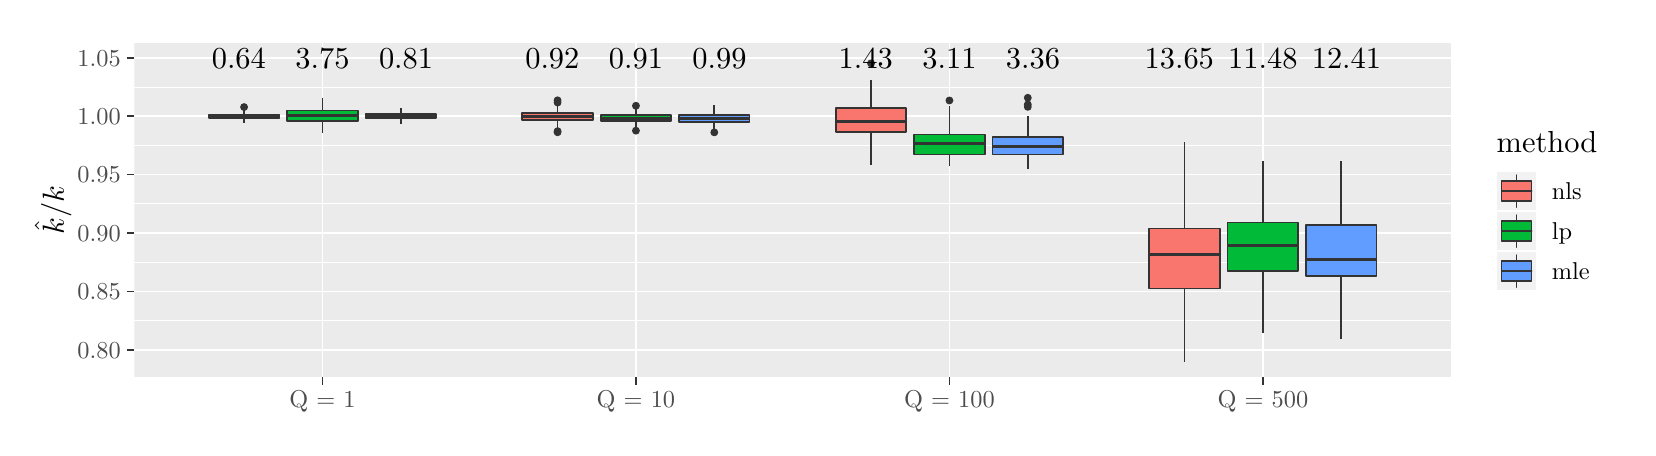
\begin{tikzpicture}[x=1pt,y=1pt]
\definecolor{fillColor}{RGB}{255,255,255}
\path[use as bounding box,fill=fillColor,fill opacity=0.00] (0,0) rectangle (578.16,144.54);
\begin{scope}
\path[clip] (  0.00,  0.00) rectangle (578.16,144.54);
\definecolor{drawColor}{RGB}{255,255,255}
\definecolor{fillColor}{RGB}{255,255,255}

\path[draw=drawColor,line width= 0.6pt,line join=round,line cap=round,fill=fillColor] (  0.00,  0.00) rectangle (578.16,144.54);
\end{scope}
\begin{scope}
\path[clip] ( 38.56, 18.22) rectangle (514.31,139.04);
\definecolor{fillColor}{gray}{0.92}

\path[fill=fillColor] ( 38.56, 18.22) rectangle (514.31,139.04);
\definecolor{drawColor}{RGB}{255,255,255}

\path[draw=drawColor,line width= 0.3pt,line join=round] ( 38.56, 38.69) --
	(514.31, 38.69);

\path[draw=drawColor,line width= 0.3pt,line join=round] ( 38.56, 59.80) --
	(514.31, 59.80);

\path[draw=drawColor,line width= 0.3pt,line join=round] ( 38.56, 80.91) --
	(514.31, 80.91);

\path[draw=drawColor,line width= 0.3pt,line join=round] ( 38.56,102.02) --
	(514.31,102.02);

\path[draw=drawColor,line width= 0.3pt,line join=round] ( 38.56,123.13) --
	(514.31,123.13);

\path[draw=drawColor,line width= 0.6pt,line join=round] ( 38.56, 28.13) --
	(514.31, 28.13);

\path[draw=drawColor,line width= 0.6pt,line join=round] ( 38.56, 49.24) --
	(514.31, 49.24);

\path[draw=drawColor,line width= 0.6pt,line join=round] ( 38.56, 70.35) --
	(514.31, 70.35);

\path[draw=drawColor,line width= 0.6pt,line join=round] ( 38.56, 91.46) --
	(514.31, 91.46);

\path[draw=drawColor,line width= 0.6pt,line join=round] ( 38.56,112.57) --
	(514.31,112.57);

\path[draw=drawColor,line width= 0.6pt,line join=round] ( 38.56,133.68) --
	(514.31,133.68);

\path[draw=drawColor,line width= 0.6pt,line join=round] (106.52, 18.22) --
	(106.52,139.04);

\path[draw=drawColor,line width= 0.6pt,line join=round] (219.79, 18.22) --
	(219.79,139.04);

\path[draw=drawColor,line width= 0.6pt,line join=round] (333.07, 18.22) --
	(333.07,139.04);

\path[draw=drawColor,line width= 0.6pt,line join=round] (446.34, 18.22) --
	(446.34,139.04);
\definecolor{drawColor}{gray}{0.20}
\definecolor{fillColor}{gray}{0.20}

\path[draw=drawColor,line width= 0.4pt,line join=round,line cap=round,fill=fillColor] ( 78.20,115.84) circle (  1.21);

\path[draw=drawColor,line width= 0.6pt,line join=round] ( 78.20,113.16) -- ( 78.20,114.96);

\path[draw=drawColor,line width= 0.6pt,line join=round] ( 78.20,111.95) -- ( 78.20,110.26);
\definecolor{fillColor}{RGB}{248,118,109}

\path[draw=drawColor,line width= 0.6pt,line join=round,line cap=round,fill=fillColor] ( 65.46,113.16) --
	( 65.46,111.95) --
	( 90.94,111.95) --
	( 90.94,113.16) --
	( 65.46,113.16) --
	cycle;

\path[draw=drawColor,line width= 1.1pt,line join=round] ( 65.46,112.53) -- ( 90.94,112.53);

\path[draw=drawColor,line width= 0.6pt,line join=round] (106.52,114.61) -- (106.52,119.28);

\path[draw=drawColor,line width= 0.6pt,line join=round] (106.52,110.92) -- (106.52,106.46);
\definecolor{fillColor}{RGB}{0,186,56}

\path[draw=drawColor,line width= 0.6pt,line join=round,line cap=round,fill=fillColor] ( 93.78,114.61) --
	( 93.78,110.92) --
	(119.26,110.92) --
	(119.26,114.61) --
	( 93.78,114.61) --
	cycle;

\path[draw=drawColor,line width= 1.1pt,line join=round] ( 93.78,112.63) -- (119.26,112.63);

\path[draw=drawColor,line width= 0.6pt,line join=round] (134.84,113.41) -- (134.84,115.64);

\path[draw=drawColor,line width= 0.6pt,line join=round] (134.84,111.90) -- (134.84,109.83);
\definecolor{fillColor}{RGB}{97,156,255}

\path[draw=drawColor,line width= 0.6pt,line join=round,line cap=round,fill=fillColor] (122.09,113.41) --
	(122.09,111.90) --
	(147.58,111.90) --
	(147.58,113.41) --
	(122.09,113.41) --
	cycle;

\path[draw=drawColor,line width= 1.1pt,line join=round] (122.09,112.45) -- (147.58,112.45);
\definecolor{fillColor}{gray}{0.20}

\path[draw=drawColor,line width= 0.4pt,line join=round,line cap=round,fill=fillColor] (191.48,107.14) circle (  1.21);

\path[draw=drawColor,line width= 0.4pt,line join=round,line cap=round,fill=fillColor] (191.48,117.48) circle (  1.21);

\path[draw=drawColor,line width= 0.4pt,line join=round,line cap=round,fill=fillColor] (191.48,106.74) circle (  1.21);

\path[draw=drawColor,line width= 0.4pt,line join=round,line cap=round,fill=fillColor] (191.48,118.29) circle (  1.21);

\path[draw=drawColor,line width= 0.6pt,line join=round] (191.48,113.73) -- (191.48,116.74);

\path[draw=drawColor,line width= 0.6pt,line join=round] (191.48,111.23) -- (191.48,108.12);
\definecolor{fillColor}{RGB}{248,118,109}

\path[draw=drawColor,line width= 0.6pt,line join=round,line cap=round,fill=fillColor] (178.73,113.73) --
	(178.73,111.23) --
	(204.22,111.23) --
	(204.22,113.73) --
	(178.73,113.73) --
	cycle;

\path[draw=drawColor,line width= 1.1pt,line join=round] (178.73,112.55) -- (204.22,112.55);
\definecolor{fillColor}{gray}{0.20}

\path[draw=drawColor,line width= 0.4pt,line join=round,line cap=round,fill=fillColor] (219.79,107.32) circle (  1.21);

\path[draw=drawColor,line width= 0.4pt,line join=round,line cap=round,fill=fillColor] (219.79,116.32) circle (  1.21);

\path[draw=drawColor,line width= 0.6pt,line join=round] (219.79,112.93) -- (219.79,115.54);

\path[draw=drawColor,line width= 0.6pt,line join=round] (219.79,110.73) -- (219.79,107.48);
\definecolor{fillColor}{RGB}{0,186,56}

\path[draw=drawColor,line width= 0.6pt,line join=round,line cap=round,fill=fillColor] (207.05,112.93) --
	(207.05,110.73) --
	(232.54,110.73) --
	(232.54,112.93) --
	(207.05,112.93) --
	cycle;

\path[draw=drawColor,line width= 1.1pt,line join=round] (207.05,111.80) -- (232.54,111.80);
\definecolor{fillColor}{gray}{0.20}

\path[draw=drawColor,line width= 0.4pt,line join=round,line cap=round,fill=fillColor] (248.11,106.71) circle (  1.21);

\path[draw=drawColor,line width= 0.6pt,line join=round] (248.11,112.92) -- (248.11,116.42);

\path[draw=drawColor,line width= 0.6pt,line join=round] (248.11,110.52) -- (248.11,106.99);
\definecolor{fillColor}{RGB}{97,156,255}

\path[draw=drawColor,line width= 0.6pt,line join=round,line cap=round,fill=fillColor] (235.37,112.92) --
	(235.37,110.52) --
	(260.86,110.52) --
	(260.86,112.92) --
	(235.37,112.92) --
	cycle;

\path[draw=drawColor,line width= 1.1pt,line join=round] (235.37,111.89) -- (260.86,111.89);
\definecolor{fillColor}{gray}{0.20}

\path[draw=drawColor,line width= 0.4pt,line join=round,line cap=round,fill=fillColor] (304.75,131.64) circle (  1.21);

\path[draw=drawColor,line width= 0.6pt,line join=round] (304.75,115.44) -- (304.75,125.75);

\path[draw=drawColor,line width= 0.6pt,line join=round] (304.75,106.91) -- (304.75, 94.74);
\definecolor{fillColor}{RGB}{248,118,109}

\path[draw=drawColor,line width= 0.6pt,line join=round,line cap=round,fill=fillColor] (292.01,115.44) --
	(292.01,106.91) --
	(317.49,106.91) --
	(317.49,115.44) --
	(292.01,115.44) --
	cycle;

\path[draw=drawColor,line width= 1.1pt,line join=round] (292.01,110.75) -- (317.49,110.75);
\definecolor{fillColor}{gray}{0.20}

\path[draw=drawColor,line width= 0.4pt,line join=round,line cap=round,fill=fillColor] (333.07,118.23) circle (  1.21);

\path[draw=drawColor,line width= 0.6pt,line join=round] (333.07,105.94) -- (333.07,116.09);

\path[draw=drawColor,line width= 0.6pt,line join=round] (333.07, 98.65) -- (333.07, 94.39);
\definecolor{fillColor}{RGB}{0,186,56}

\path[draw=drawColor,line width= 0.6pt,line join=round,line cap=round,fill=fillColor] (320.33,105.94) --
	(320.33, 98.65) --
	(345.81, 98.65) --
	(345.81,105.94) --
	(320.33,105.94) --
	cycle;

\path[draw=drawColor,line width= 1.1pt,line join=round] (320.33,102.71) -- (345.81,102.71);
\definecolor{fillColor}{gray}{0.20}

\path[draw=drawColor,line width= 0.4pt,line join=round,line cap=round,fill=fillColor] (361.39,115.92) circle (  1.21);

\path[draw=drawColor,line width= 0.4pt,line join=round,line cap=round,fill=fillColor] (361.39,116.80) circle (  1.21);

\path[draw=drawColor,line width= 0.4pt,line join=round,line cap=round,fill=fillColor] (361.39,119.21) circle (  1.21);

\path[draw=drawColor,line width= 0.6pt,line join=round] (361.39,104.95) -- (361.39,112.57);

\path[draw=drawColor,line width= 0.6pt,line join=round] (361.39, 98.75) -- (361.39, 93.57);
\definecolor{fillColor}{RGB}{97,156,255}

\path[draw=drawColor,line width= 0.6pt,line join=round,line cap=round,fill=fillColor] (348.64,104.95) --
	(348.64, 98.75) --
	(374.13, 98.75) --
	(374.13,104.95) --
	(348.64,104.95) --
	cycle;

\path[draw=drawColor,line width= 1.1pt,line join=round] (348.64,101.57) -- (374.13,101.57);

\path[draw=drawColor,line width= 0.6pt,line join=round] (418.02, 71.96) -- (418.02,103.06);

\path[draw=drawColor,line width= 0.6pt,line join=round] (418.02, 50.27) -- (418.02, 23.71);
\definecolor{fillColor}{RGB}{248,118,109}

\path[draw=drawColor,line width= 0.6pt,line join=round,line cap=round,fill=fillColor] (405.28, 71.96) --
	(405.28, 50.27) --
	(430.77, 50.27) --
	(430.77, 71.96) --
	(405.28, 71.96) --
	cycle;

\path[draw=drawColor,line width= 1.1pt,line join=round] (405.28, 62.65) -- (430.77, 62.65);

\path[draw=drawColor,line width= 0.6pt,line join=round] (446.34, 74.14) -- (446.34, 96.48);

\path[draw=drawColor,line width= 0.6pt,line join=round] (446.34, 56.68) -- (446.34, 34.03);
\definecolor{fillColor}{RGB}{0,186,56}

\path[draw=drawColor,line width= 0.6pt,line join=round,line cap=round,fill=fillColor] (433.60, 74.14) --
	(433.60, 56.68) --
	(459.09, 56.68) --
	(459.09, 74.14) --
	(433.60, 74.14) --
	cycle;

\path[draw=drawColor,line width= 1.1pt,line join=round] (433.60, 65.79) -- (459.09, 65.79);

\path[draw=drawColor,line width= 0.6pt,line join=round] (474.66, 73.22) -- (474.66, 96.48);

\path[draw=drawColor,line width= 0.6pt,line join=round] (474.66, 54.72) -- (474.66, 32.20);
\definecolor{fillColor}{RGB}{97,156,255}

\path[draw=drawColor,line width= 0.6pt,line join=round,line cap=round,fill=fillColor] (461.92, 73.22) --
	(461.92, 54.72) --
	(487.40, 54.72) --
	(487.40, 73.22) --
	(461.92, 73.22) --
	cycle;

\path[draw=drawColor,line width= 1.1pt,line join=round] (461.92, 60.83) -- (487.40, 60.83);
\definecolor{drawColor}{RGB}{0,0,0}

\node[text=drawColor,anchor=base,inner sep=0pt, outer sep=0pt, scale=  1.10] at (136.73,129.75) {0.81};

\node[text=drawColor,anchor=base,inner sep=0pt, outer sep=0pt, scale=  1.10] at (106.52,129.75) {3.75};

\node[text=drawColor,anchor=base,inner sep=0pt, outer sep=0pt, scale=  1.10] at ( 76.31,129.75) {0.64};

\node[text=drawColor,anchor=base,inner sep=0pt, outer sep=0pt, scale=  1.10] at (250.00,129.75) {0.99};

\node[text=drawColor,anchor=base,inner sep=0pt, outer sep=0pt, scale=  1.10] at (219.79,129.75) {0.91};

\node[text=drawColor,anchor=base,inner sep=0pt, outer sep=0pt, scale=  1.10] at (189.59,129.75) {0.92};

\node[text=drawColor,anchor=base,inner sep=0pt, outer sep=0pt, scale=  1.10] at (363.28,129.75) {3.36};

\node[text=drawColor,anchor=base,inner sep=0pt, outer sep=0pt, scale=  1.10] at (333.07,129.75) {3.11};

\node[text=drawColor,anchor=base,inner sep=0pt, outer sep=0pt, scale=  1.10] at (302.86,129.75) {1.43};

\node[text=drawColor,anchor=base,inner sep=0pt, outer sep=0pt, scale=  1.10] at (476.55,129.75) {12.41};

\node[text=drawColor,anchor=base,inner sep=0pt, outer sep=0pt, scale=  1.10] at (446.34,129.75) {11.48};

\node[text=drawColor,anchor=base,inner sep=0pt, outer sep=0pt, scale=  1.10] at (416.14,129.75) {13.65};
\end{scope}
\begin{scope}
\path[clip] (  0.00,  0.00) rectangle (578.16,144.54);
\definecolor{drawColor}{gray}{0.30}

\node[text=drawColor,anchor=base east,inner sep=0pt, outer sep=0pt, scale=  0.88] at ( 33.61, 25.10) {0.80};

\node[text=drawColor,anchor=base east,inner sep=0pt, outer sep=0pt, scale=  0.88] at ( 33.61, 46.21) {0.85};

\node[text=drawColor,anchor=base east,inner sep=0pt, outer sep=0pt, scale=  0.88] at ( 33.61, 67.32) {0.90};

\node[text=drawColor,anchor=base east,inner sep=0pt, outer sep=0pt, scale=  0.88] at ( 33.61, 88.43) {0.95};

\node[text=drawColor,anchor=base east,inner sep=0pt, outer sep=0pt, scale=  0.88] at ( 33.61,109.54) {1.00};

\node[text=drawColor,anchor=base east,inner sep=0pt, outer sep=0pt, scale=  0.88] at ( 33.61,130.65) {1.05};
\end{scope}
\begin{scope}
\path[clip] (  0.00,  0.00) rectangle (578.16,144.54);
\definecolor{drawColor}{gray}{0.20}

\path[draw=drawColor,line width= 0.6pt,line join=round] ( 35.81, 28.13) --
	( 38.56, 28.13);

\path[draw=drawColor,line width= 0.6pt,line join=round] ( 35.81, 49.24) --
	( 38.56, 49.24);

\path[draw=drawColor,line width= 0.6pt,line join=round] ( 35.81, 70.35) --
	( 38.56, 70.35);

\path[draw=drawColor,line width= 0.6pt,line join=round] ( 35.81, 91.46) --
	( 38.56, 91.46);

\path[draw=drawColor,line width= 0.6pt,line join=round] ( 35.81,112.57) --
	( 38.56,112.57);

\path[draw=drawColor,line width= 0.6pt,line join=round] ( 35.81,133.68) --
	( 38.56,133.68);
\end{scope}
\begin{scope}
\path[clip] (  0.00,  0.00) rectangle (578.16,144.54);
\definecolor{drawColor}{gray}{0.20}

\path[draw=drawColor,line width= 0.6pt,line join=round] (106.52, 15.47) --
	(106.52, 18.22);

\path[draw=drawColor,line width= 0.6pt,line join=round] (219.79, 15.47) --
	(219.79, 18.22);

\path[draw=drawColor,line width= 0.6pt,line join=round] (333.07, 15.47) --
	(333.07, 18.22);

\path[draw=drawColor,line width= 0.6pt,line join=round] (446.34, 15.47) --
	(446.34, 18.22);
\end{scope}
\begin{scope}
\path[clip] (  0.00,  0.00) rectangle (578.16,144.54);
\definecolor{drawColor}{gray}{0.30}

\node[text=drawColor,anchor=base,inner sep=0pt, outer sep=0pt, scale=  0.88] at (106.52,  7.21) {Q = 1};

\node[text=drawColor,anchor=base,inner sep=0pt, outer sep=0pt, scale=  0.88] at (219.79,  7.21) {Q = 10};

\node[text=drawColor,anchor=base,inner sep=0pt, outer sep=0pt, scale=  0.88] at (333.07,  7.21) {Q = 100};

\node[text=drawColor,anchor=base,inner sep=0pt, outer sep=0pt, scale=  0.88] at (446.34,  7.21) {Q = 500};
\end{scope}
\begin{scope}
\path[clip] (  0.00,  0.00) rectangle (578.16,144.54);
\definecolor{drawColor}{RGB}{0,0,0}

\node[text=drawColor,rotate= 90.00,anchor=base,inner sep=0pt, outer sep=0pt, scale=  1.10] at ( 13.08, 78.63) {$\hat{k}/k$};
\end{scope}
\begin{scope}
\path[clip] (  0.00,  0.00) rectangle (578.16,144.54);
\definecolor{fillColor}{RGB}{255,255,255}

\path[fill=fillColor] (525.31, 43.84) rectangle (572.66,113.42);
\end{scope}
\begin{scope}
\path[clip] (  0.00,  0.00) rectangle (578.16,144.54);
\definecolor{drawColor}{RGB}{0,0,0}

\node[text=drawColor,anchor=base west,inner sep=0pt, outer sep=0pt, scale=  1.10] at (530.81, 99.27) {method};
\end{scope}
\begin{scope}
\path[clip] (  0.00,  0.00) rectangle (578.16,144.54);
\definecolor{drawColor}{RGB}{255,255,255}
\definecolor{fillColor}{gray}{0.95}

\path[draw=drawColor,line width= 0.6pt,line join=round,line cap=round,fill=fillColor] (530.81, 78.25) rectangle (545.26, 92.70);
\end{scope}
\begin{scope}
\path[clip] (  0.00,  0.00) rectangle (578.16,144.54);
\definecolor{drawColor}{gray}{0.20}

\path[draw=drawColor,line width= 0.6pt,line join=round,line cap=round] (538.03, 79.70) --
	(538.03, 81.86);

\path[draw=drawColor,line width= 0.6pt,line join=round,line cap=round] (538.03, 89.09) --
	(538.03, 91.26);
\definecolor{fillColor}{RGB}{248,118,109}

\path[draw=drawColor,line width= 0.6pt,line join=round,line cap=round,fill=fillColor] (532.61, 81.86) rectangle (543.45, 89.09);

\path[draw=drawColor,line width= 0.6pt,line join=round,line cap=round] (532.61, 85.48) --
	(543.45, 85.48);
\end{scope}
\begin{scope}
\path[clip] (  0.00,  0.00) rectangle (578.16,144.54);
\definecolor{drawColor}{RGB}{255,255,255}
\definecolor{fillColor}{gray}{0.95}

\path[draw=drawColor,line width= 0.6pt,line join=round,line cap=round,fill=fillColor] (530.81, 63.80) rectangle (545.26, 78.25);
\end{scope}
\begin{scope}
\path[clip] (  0.00,  0.00) rectangle (578.16,144.54);
\definecolor{drawColor}{gray}{0.20}

\path[draw=drawColor,line width= 0.6pt,line join=round,line cap=round] (538.03, 65.24) --
	(538.03, 67.41);

\path[draw=drawColor,line width= 0.6pt,line join=round,line cap=round] (538.03, 74.64) --
	(538.03, 76.81);
\definecolor{fillColor}{RGB}{0,186,56}

\path[draw=drawColor,line width= 0.6pt,line join=round,line cap=round,fill=fillColor] (532.61, 67.41) rectangle (543.45, 74.64);

\path[draw=drawColor,line width= 0.6pt,line join=round,line cap=round] (532.61, 71.02) --
	(543.45, 71.02);
\end{scope}
\begin{scope}
\path[clip] (  0.00,  0.00) rectangle (578.16,144.54);
\definecolor{drawColor}{RGB}{255,255,255}
\definecolor{fillColor}{gray}{0.95}

\path[draw=drawColor,line width= 0.6pt,line join=round,line cap=round,fill=fillColor] (530.81, 49.34) rectangle (545.26, 63.80);
\end{scope}
\begin{scope}
\path[clip] (  0.00,  0.00) rectangle (578.16,144.54);
\definecolor{drawColor}{gray}{0.20}

\path[draw=drawColor,line width= 0.6pt,line join=round,line cap=round] (538.03, 50.79) --
	(538.03, 52.96);

\path[draw=drawColor,line width= 0.6pt,line join=round,line cap=round] (538.03, 60.18) --
	(538.03, 62.35);
\definecolor{fillColor}{RGB}{97,156,255}

\path[draw=drawColor,line width= 0.6pt,line join=round,line cap=round,fill=fillColor] (532.61, 52.96) rectangle (543.45, 60.18);

\path[draw=drawColor,line width= 0.6pt,line join=round,line cap=round] (532.61, 56.57) --
	(543.45, 56.57);
\end{scope}
\begin{scope}
\path[clip] (  0.00,  0.00) rectangle (578.16,144.54);
\definecolor{drawColor}{RGB}{0,0,0}

\node[text=drawColor,anchor=base west,inner sep=0pt, outer sep=0pt, scale=  0.88] at (550.76, 82.45) {nls};
\end{scope}
\begin{scope}
\path[clip] (  0.00,  0.00) rectangle (578.16,144.54);
\definecolor{drawColor}{RGB}{0,0,0}

\node[text=drawColor,anchor=base west,inner sep=0pt, outer sep=0pt, scale=  0.88] at (550.76, 67.99) {lp};
\end{scope}
\begin{scope}
\path[clip] (  0.00,  0.00) rectangle (578.16,144.54);
\definecolor{drawColor}{RGB}{0,0,0}

\node[text=drawColor,anchor=base west,inner sep=0pt, outer sep=0pt, scale=  0.88] at (550.76, 53.54) {mle};
\end{scope}
\end{tikzpicture}
}
  \end{subfigure}
  \hfill
  \begin{subfigure}
    \centering
    \resizebox{1.1\linewidth}{!}{% Created by tikzDevice version 0.12.3 on 2019-09-26 18:31:14
% !TEX encoding = UTF-8 Unicode
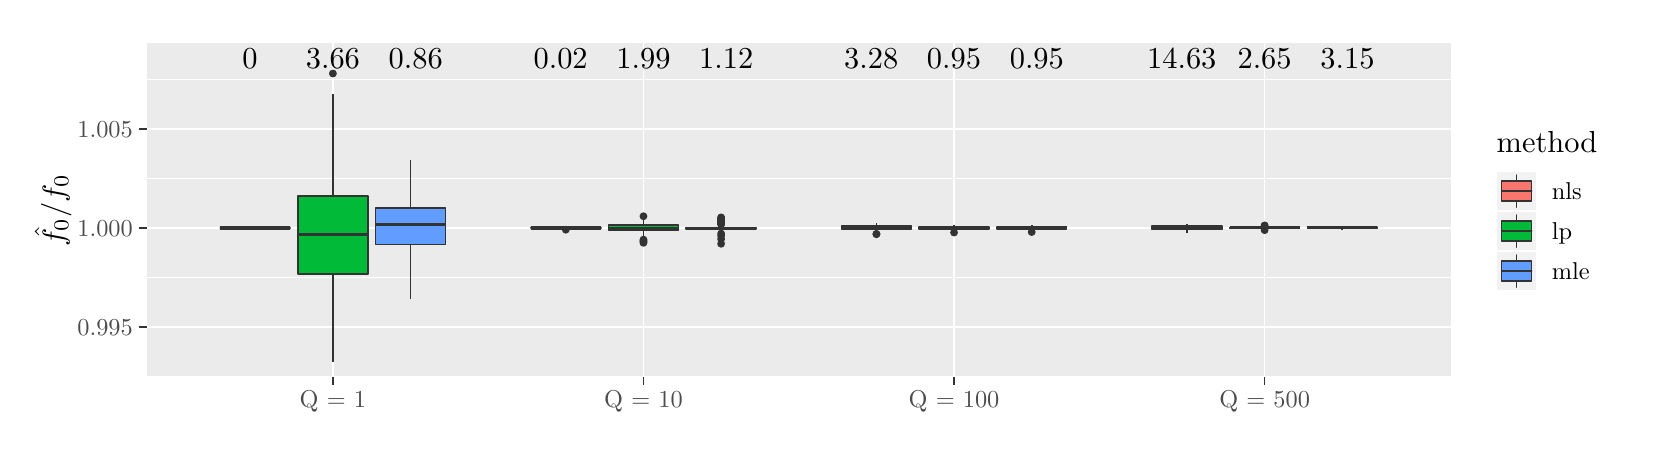
\begin{tikzpicture}[x=1pt,y=1pt]
\definecolor{fillColor}{RGB}{255,255,255}
\path[use as bounding box,fill=fillColor,fill opacity=0.00] (0,0) rectangle (578.16,144.54);
\begin{scope}
\path[clip] (  0.00,  0.00) rectangle (578.16,144.54);
\definecolor{drawColor}{RGB}{255,255,255}
\definecolor{fillColor}{RGB}{255,255,255}

\path[draw=drawColor,line width= 0.6pt,line join=round,line cap=round,fill=fillColor] (  0.00,  0.00) rectangle (578.16,144.54);
\end{scope}
\begin{scope}
\path[clip] ( 42.95, 18.22) rectangle (514.31,139.04);
\definecolor{fillColor}{gray}{0.92}

\path[fill=fillColor] ( 42.95, 18.22) rectangle (514.31,139.04);
\definecolor{drawColor}{RGB}{255,255,255}

\path[draw=drawColor,line width= 0.3pt,line join=round] ( 42.95, 18.51) --
	(514.31, 18.51);

\path[draw=drawColor,line width= 0.3pt,line join=round] ( 42.95, 54.27) --
	(514.31, 54.27);

\path[draw=drawColor,line width= 0.3pt,line join=round] ( 42.95, 90.03) --
	(514.31, 90.03);

\path[draw=drawColor,line width= 0.3pt,line join=round] ( 42.95,125.78) --
	(514.31,125.78);

\path[draw=drawColor,line width= 0.6pt,line join=round] ( 42.95, 36.39) --
	(514.31, 36.39);

\path[draw=drawColor,line width= 0.6pt,line join=round] ( 42.95, 72.15) --
	(514.31, 72.15);

\path[draw=drawColor,line width= 0.6pt,line join=round] ( 42.95,107.91) --
	(514.31,107.91);

\path[draw=drawColor,line width= 0.6pt,line join=round] (110.29, 18.22) --
	(110.29,139.04);

\path[draw=drawColor,line width= 0.6pt,line join=round] (222.52, 18.22) --
	(222.52,139.04);

\path[draw=drawColor,line width= 0.6pt,line join=round] (334.74, 18.22) --
	(334.74,139.04);

\path[draw=drawColor,line width= 0.6pt,line join=round] (446.97, 18.22) --
	(446.97,139.04);
\definecolor{drawColor}{gray}{0.20}

\path[draw=drawColor,line width= 0.6pt,line join=round] ( 82.23, 72.15) -- ( 82.23, 72.15);

\path[draw=drawColor,line width= 0.6pt,line join=round] ( 82.23, 72.15) -- ( 82.23, 72.15);
\definecolor{fillColor}{RGB}{248,118,109}

\path[draw=drawColor,line width= 0.6pt,line join=round,line cap=round,fill=fillColor] ( 69.61, 72.15) --
	( 69.61, 72.15) --
	( 94.86, 72.15) --
	( 94.86, 72.15) --
	( 69.61, 72.15) --
	cycle;

\path[draw=drawColor,line width= 1.1pt,line join=round] ( 69.61, 72.15) -- ( 94.86, 72.15);
\definecolor{fillColor}{gray}{0.20}

\path[draw=drawColor,line width= 0.4pt,line join=round,line cap=round,fill=fillColor] (110.29,127.97) circle (  1.21);

\path[draw=drawColor,line width= 0.6pt,line join=round] (110.29, 83.73) -- (110.29,120.40);

\path[draw=drawColor,line width= 0.6pt,line join=round] (110.29, 55.49) -- (110.29, 23.71);
\definecolor{fillColor}{RGB}{0,186,56}

\path[draw=drawColor,line width= 0.6pt,line join=round,line cap=round,fill=fillColor] ( 97.66, 83.73) --
	( 97.66, 55.49) --
	(122.92, 55.49) --
	(122.92, 83.73) --
	( 97.66, 83.73) --
	cycle;

\path[draw=drawColor,line width= 1.1pt,line join=round] ( 97.66, 69.85) -- (122.92, 69.85);

\path[draw=drawColor,line width= 0.6pt,line join=round] (138.35, 79.48) -- (138.35, 96.89);

\path[draw=drawColor,line width= 0.6pt,line join=round] (138.35, 66.14) -- (138.35, 46.49);
\definecolor{fillColor}{RGB}{97,156,255}

\path[draw=drawColor,line width= 0.6pt,line join=round,line cap=round,fill=fillColor] (125.72, 79.48) --
	(125.72, 66.14) --
	(150.97, 66.14) --
	(150.97, 79.48) --
	(125.72, 79.48) --
	cycle;

\path[draw=drawColor,line width= 1.1pt,line join=round] (125.72, 73.55) -- (150.97, 73.55);
\definecolor{fillColor}{gray}{0.20}

\path[draw=drawColor,line width= 0.4pt,line join=round,line cap=round,fill=fillColor] (194.46, 71.54) circle (  1.21);

\path[draw=drawColor,line width= 0.6pt,line join=round] (194.46, 72.28) -- (194.46, 72.52);

\path[draw=drawColor,line width= 0.6pt,line join=round] (194.46, 72.05) -- (194.46, 71.85);
\definecolor{fillColor}{RGB}{248,118,109}

\path[draw=drawColor,line width= 0.6pt,line join=round,line cap=round,fill=fillColor] (181.83, 72.28) --
	(181.83, 72.05) --
	(207.09, 72.05) --
	(207.09, 72.28) --
	(181.83, 72.28) --
	cycle;

\path[draw=drawColor,line width= 1.1pt,line join=round] (181.83, 72.15) -- (207.09, 72.15);
\definecolor{fillColor}{gray}{0.20}

\path[draw=drawColor,line width= 0.4pt,line join=round,line cap=round,fill=fillColor] (222.52, 67.94) circle (  1.21);

\path[draw=drawColor,line width= 0.4pt,line join=round,line cap=round,fill=fillColor] (222.52, 67.55) circle (  1.21);

\path[draw=drawColor,line width= 0.4pt,line join=round,line cap=round,fill=fillColor] (222.52, 66.79) circle (  1.21);

\path[draw=drawColor,line width= 0.4pt,line join=round,line cap=round,fill=fillColor] (222.52, 76.40) circle (  1.21);

\path[draw=drawColor,line width= 0.4pt,line join=round,line cap=round,fill=fillColor] (222.52, 67.19) circle (  1.21);

\path[draw=drawColor,line width= 0.6pt,line join=round] (222.52, 73.31) -- (222.52, 75.71);

\path[draw=drawColor,line width= 0.6pt,line join=round] (222.52, 71.26) -- (222.52, 68.48);
\definecolor{fillColor}{RGB}{0,186,56}

\path[draw=drawColor,line width= 0.6pt,line join=round,line cap=round,fill=fillColor] (209.89, 73.31) --
	(209.89, 71.26) --
	(235.14, 71.26) --
	(235.14, 73.31) --
	(209.89, 73.31) --
	cycle;

\path[draw=drawColor,line width= 1.1pt,line join=round] (209.89, 72.00) -- (235.14, 72.00);
\definecolor{fillColor}{gray}{0.20}

\path[draw=drawColor,line width= 0.4pt,line join=round,line cap=round,fill=fillColor] (250.57, 74.64) circle (  1.21);

\path[draw=drawColor,line width= 0.4pt,line join=round,line cap=round,fill=fillColor] (250.57, 73.70) circle (  1.21);

\path[draw=drawColor,line width= 0.4pt,line join=round,line cap=round,fill=fillColor] (250.57, 75.39) circle (  1.21);

\path[draw=drawColor,line width= 0.4pt,line join=round,line cap=round,fill=fillColor] (250.57, 75.55) circle (  1.21);

\path[draw=drawColor,line width= 0.4pt,line join=round,line cap=round,fill=fillColor] (250.57, 73.83) circle (  1.21);

\path[draw=drawColor,line width= 0.4pt,line join=round,line cap=round,fill=fillColor] (250.57, 75.16) circle (  1.21);

\path[draw=drawColor,line width= 0.4pt,line join=round,line cap=round,fill=fillColor] (250.57, 70.13) circle (  1.21);

\path[draw=drawColor,line width= 0.4pt,line join=round,line cap=round,fill=fillColor] (250.57, 69.34) circle (  1.21);

\path[draw=drawColor,line width= 0.4pt,line join=round,line cap=round,fill=fillColor] (250.57, 75.26) circle (  1.21);

\path[draw=drawColor,line width= 0.4pt,line join=round,line cap=round,fill=fillColor] (250.57, 73.87) circle (  1.21);

\path[draw=drawColor,line width= 0.4pt,line join=round,line cap=round,fill=fillColor] (250.57, 66.46) circle (  1.21);

\path[draw=drawColor,line width= 0.4pt,line join=round,line cap=round,fill=fillColor] (250.57, 74.50) circle (  1.21);

\path[draw=drawColor,line width= 0.4pt,line join=round,line cap=round,fill=fillColor] (250.57, 74.43) circle (  1.21);

\path[draw=drawColor,line width= 0.4pt,line join=round,line cap=round,fill=fillColor] (250.57, 68.15) circle (  1.21);

\path[draw=drawColor,line width= 0.4pt,line join=round,line cap=round,fill=fillColor] (250.57, 75.99) circle (  1.21);

\path[draw=drawColor,line width= 0.4pt,line join=round,line cap=round,fill=fillColor] (250.57, 75.49) circle (  1.21);

\path[draw=drawColor,line width= 0.4pt,line join=round,line cap=round,fill=fillColor] (250.57, 73.50) circle (  1.21);

\path[draw=drawColor,line width= 0.4pt,line join=round,line cap=round,fill=fillColor] (250.57, 74.89) circle (  1.21);

\path[draw=drawColor,line width= 0.4pt,line join=round,line cap=round,fill=fillColor] (250.57, 74.01) circle (  1.21);

\path[draw=drawColor,line width= 0.4pt,line join=round,line cap=round,fill=fillColor] (250.57, 75.45) circle (  1.21);

\path[draw=drawColor,line width= 0.4pt,line join=round,line cap=round,fill=fillColor] (250.57, 74.77) circle (  1.21);

\path[draw=drawColor,line width= 0.6pt,line join=round] (250.57, 72.37) -- (250.57, 72.98);

\path[draw=drawColor,line width= 0.6pt,line join=round] (250.57, 71.67) -- (250.57, 70.86);
\definecolor{fillColor}{RGB}{97,156,255}

\path[draw=drawColor,line width= 0.6pt,line join=round,line cap=round,fill=fillColor] (237.95, 72.37) --
	(237.95, 71.67) --
	(263.20, 71.67) --
	(263.20, 72.37) --
	(237.95, 72.37) --
	cycle;

\path[draw=drawColor,line width= 1.1pt,line join=round] (237.95, 72.01) -- (263.20, 72.01);
\definecolor{fillColor}{gray}{0.20}

\path[draw=drawColor,line width= 0.4pt,line join=round,line cap=round,fill=fillColor] (306.69, 69.90) circle (  1.21);

\path[draw=drawColor,line width= 0.4pt,line join=round,line cap=round,fill=fillColor] (306.69, 70.03) circle (  1.21);

\path[draw=drawColor,line width= 0.6pt,line join=round] (306.69, 72.81) -- (306.69, 74.08);

\path[draw=drawColor,line width= 0.6pt,line join=round] (306.69, 71.73) -- (306.69, 70.50);
\definecolor{fillColor}{RGB}{248,118,109}

\path[draw=drawColor,line width= 0.6pt,line join=round,line cap=round,fill=fillColor] (294.06, 72.81) --
	(294.06, 71.73) --
	(319.31, 71.73) --
	(319.31, 72.81) --
	(294.06, 72.81) --
	cycle;

\path[draw=drawColor,line width= 1.1pt,line join=round] (294.06, 72.17) -- (319.31, 72.17);
\definecolor{fillColor}{gray}{0.20}

\path[draw=drawColor,line width= 0.4pt,line join=round,line cap=round,fill=fillColor] (334.74, 70.52) circle (  1.21);

\path[draw=drawColor,line width= 0.6pt,line join=round] (334.74, 72.51) -- (334.74, 73.17);

\path[draw=drawColor,line width= 0.6pt,line join=round] (334.74, 71.88) -- (334.74, 71.09);
\definecolor{fillColor}{RGB}{0,186,56}

\path[draw=drawColor,line width= 0.6pt,line join=round,line cap=round,fill=fillColor] (322.12, 72.51) --
	(322.12, 71.88) --
	(347.37, 71.88) --
	(347.37, 72.51) --
	(322.12, 72.51) --
	cycle;

\path[draw=drawColor,line width= 1.1pt,line join=round] (322.12, 72.23) -- (347.37, 72.23);
\definecolor{fillColor}{gray}{0.20}

\path[draw=drawColor,line width= 0.4pt,line join=round,line cap=round,fill=fillColor] (362.80, 70.70) circle (  1.21);

\path[draw=drawColor,line width= 0.6pt,line join=round] (362.80, 72.52) -- (362.80, 73.13);

\path[draw=drawColor,line width= 0.6pt,line join=round] (362.80, 71.87) -- (362.80, 71.19);
\definecolor{fillColor}{RGB}{97,156,255}

\path[draw=drawColor,line width= 0.6pt,line join=round,line cap=round,fill=fillColor] (350.18, 72.52) --
	(350.18, 71.87) --
	(375.43, 71.87) --
	(375.43, 72.52) --
	(350.18, 72.52) --
	cycle;

\path[draw=drawColor,line width= 1.1pt,line join=round] (350.18, 72.23) -- (375.43, 72.23);

\path[draw=drawColor,line width= 0.6pt,line join=round] (418.91, 72.80) -- (418.91, 73.64);

\path[draw=drawColor,line width= 0.6pt,line join=round] (418.91, 71.63) -- (418.91, 70.47);
\definecolor{fillColor}{RGB}{248,118,109}

\path[draw=drawColor,line width= 0.6pt,line join=round,line cap=round,fill=fillColor] (406.29, 72.80) --
	(406.29, 71.63) --
	(431.54, 71.63) --
	(431.54, 72.80) --
	(406.29, 72.80) --
	cycle;

\path[draw=drawColor,line width= 1.1pt,line join=round] (406.29, 72.13) -- (431.54, 72.13);
\definecolor{fillColor}{gray}{0.20}

\path[draw=drawColor,line width= 0.4pt,line join=round,line cap=round,fill=fillColor] (446.97, 73.00) circle (  1.21);

\path[draw=drawColor,line width= 0.4pt,line join=round,line cap=round,fill=fillColor] (446.97, 73.06) circle (  1.21);

\path[draw=drawColor,line width= 0.4pt,line join=round,line cap=round,fill=fillColor] (446.97, 71.37) circle (  1.21);

\path[draw=drawColor,line width= 0.6pt,line join=round] (446.97, 72.35) -- (446.97, 72.89);

\path[draw=drawColor,line width= 0.6pt,line join=round] (446.97, 71.97) -- (446.97, 71.61);
\definecolor{fillColor}{RGB}{0,186,56}

\path[draw=drawColor,line width= 0.6pt,line join=round,line cap=round,fill=fillColor] (434.35, 72.35) --
	(434.35, 71.97) --
	(459.60, 71.97) --
	(459.60, 72.35) --
	(434.35, 72.35) --
	cycle;

\path[draw=drawColor,line width= 1.1pt,line join=round] (434.35, 72.16) -- (459.60, 72.16);

\path[draw=drawColor,line width= 0.6pt,line join=round] (475.03, 72.50) -- (475.03, 72.99);

\path[draw=drawColor,line width= 0.6pt,line join=round] (475.03, 71.98) -- (475.03, 71.52);
\definecolor{fillColor}{RGB}{97,156,255}

\path[draw=drawColor,line width= 0.6pt,line join=round,line cap=round,fill=fillColor] (462.40, 72.50) --
	(462.40, 71.98) --
	(487.65, 71.98) --
	(487.65, 72.50) --
	(462.40, 72.50) --
	cycle;

\path[draw=drawColor,line width= 1.1pt,line join=round] (462.40, 72.27) -- (487.65, 72.27);
\definecolor{drawColor}{RGB}{0,0,0}

\node[text=drawColor,anchor=base,inner sep=0pt, outer sep=0pt, scale=  1.10] at (140.22,129.75) {0.86};

\node[text=drawColor,anchor=base,inner sep=0pt, outer sep=0pt, scale=  1.10] at (110.29,129.75) {3.66};

\node[text=drawColor,anchor=base,inner sep=0pt, outer sep=0pt, scale=  1.10] at ( 80.36,129.75) {0};

\node[text=drawColor,anchor=base,inner sep=0pt, outer sep=0pt, scale=  1.10] at (252.44,129.75) {1.12};

\node[text=drawColor,anchor=base,inner sep=0pt, outer sep=0pt, scale=  1.10] at (222.52,129.75) {1.99};

\node[text=drawColor,anchor=base,inner sep=0pt, outer sep=0pt, scale=  1.10] at (192.59,129.75) {0.02};

\node[text=drawColor,anchor=base,inner sep=0pt, outer sep=0pt, scale=  1.10] at (364.67,129.75) {0.95};

\node[text=drawColor,anchor=base,inner sep=0pt, outer sep=0pt, scale=  1.10] at (334.74,129.75) {0.95};

\node[text=drawColor,anchor=base,inner sep=0pt, outer sep=0pt, scale=  1.10] at (304.82,129.75) {3.28};

\node[text=drawColor,anchor=base,inner sep=0pt, outer sep=0pt, scale=  1.10] at (476.90,129.75) {3.15};

\node[text=drawColor,anchor=base,inner sep=0pt, outer sep=0pt, scale=  1.10] at (446.97,129.75) {2.65};

\node[text=drawColor,anchor=base,inner sep=0pt, outer sep=0pt, scale=  1.10] at (417.04,129.75) {14.63};
\end{scope}
\begin{scope}
\path[clip] (  0.00,  0.00) rectangle (578.16,144.54);
\definecolor{drawColor}{gray}{0.30}

\node[text=drawColor,anchor=base east,inner sep=0pt, outer sep=0pt, scale=  0.88] at ( 38.00, 33.36) {0.995};

\node[text=drawColor,anchor=base east,inner sep=0pt, outer sep=0pt, scale=  0.88] at ( 38.00, 69.12) {1.000};

\node[text=drawColor,anchor=base east,inner sep=0pt, outer sep=0pt, scale=  0.88] at ( 38.00,104.88) {1.005};
\end{scope}
\begin{scope}
\path[clip] (  0.00,  0.00) rectangle (578.16,144.54);
\definecolor{drawColor}{gray}{0.20}

\path[draw=drawColor,line width= 0.6pt,line join=round] ( 40.20, 36.39) --
	( 42.95, 36.39);

\path[draw=drawColor,line width= 0.6pt,line join=round] ( 40.20, 72.15) --
	( 42.95, 72.15);

\path[draw=drawColor,line width= 0.6pt,line join=round] ( 40.20,107.91) --
	( 42.95,107.91);
\end{scope}
\begin{scope}
\path[clip] (  0.00,  0.00) rectangle (578.16,144.54);
\definecolor{drawColor}{gray}{0.20}

\path[draw=drawColor,line width= 0.6pt,line join=round] (110.29, 15.47) --
	(110.29, 18.22);

\path[draw=drawColor,line width= 0.6pt,line join=round] (222.52, 15.47) --
	(222.52, 18.22);

\path[draw=drawColor,line width= 0.6pt,line join=round] (334.74, 15.47) --
	(334.74, 18.22);

\path[draw=drawColor,line width= 0.6pt,line join=round] (446.97, 15.47) --
	(446.97, 18.22);
\end{scope}
\begin{scope}
\path[clip] (  0.00,  0.00) rectangle (578.16,144.54);
\definecolor{drawColor}{gray}{0.30}

\node[text=drawColor,anchor=base,inner sep=0pt, outer sep=0pt, scale=  0.88] at (110.29,  7.21) {Q = 1};

\node[text=drawColor,anchor=base,inner sep=0pt, outer sep=0pt, scale=  0.88] at (222.52,  7.21) {Q = 10};

\node[text=drawColor,anchor=base,inner sep=0pt, outer sep=0pt, scale=  0.88] at (334.74,  7.21) {Q = 100};

\node[text=drawColor,anchor=base,inner sep=0pt, outer sep=0pt, scale=  0.88] at (446.97,  7.21) {Q = 500};
\end{scope}
\begin{scope}
\path[clip] (  0.00,  0.00) rectangle (578.16,144.54);
\definecolor{drawColor}{RGB}{0,0,0}

\node[text=drawColor,rotate= 90.00,anchor=base,inner sep=0pt, outer sep=0pt, scale=  1.10] at ( 13.08, 78.63) {$\hat{f_0}/f_0$};
\end{scope}
\begin{scope}
\path[clip] (  0.00,  0.00) rectangle (578.16,144.54);
\definecolor{fillColor}{RGB}{255,255,255}

\path[fill=fillColor] (525.31, 43.84) rectangle (572.66,113.42);
\end{scope}
\begin{scope}
\path[clip] (  0.00,  0.00) rectangle (578.16,144.54);
\definecolor{drawColor}{RGB}{0,0,0}

\node[text=drawColor,anchor=base west,inner sep=0pt, outer sep=0pt, scale=  1.10] at (530.81, 99.27) {method};
\end{scope}
\begin{scope}
\path[clip] (  0.00,  0.00) rectangle (578.16,144.54);
\definecolor{drawColor}{RGB}{255,255,255}
\definecolor{fillColor}{gray}{0.95}

\path[draw=drawColor,line width= 0.6pt,line join=round,line cap=round,fill=fillColor] (530.81, 78.25) rectangle (545.26, 92.70);
\end{scope}
\begin{scope}
\path[clip] (  0.00,  0.00) rectangle (578.16,144.54);
\definecolor{drawColor}{gray}{0.20}

\path[draw=drawColor,line width= 0.6pt,line join=round,line cap=round] (538.03, 79.70) --
	(538.03, 81.86);

\path[draw=drawColor,line width= 0.6pt,line join=round,line cap=round] (538.03, 89.09) --
	(538.03, 91.26);
\definecolor{fillColor}{RGB}{248,118,109}

\path[draw=drawColor,line width= 0.6pt,line join=round,line cap=round,fill=fillColor] (532.61, 81.86) rectangle (543.45, 89.09);

\path[draw=drawColor,line width= 0.6pt,line join=round,line cap=round] (532.61, 85.48) --
	(543.45, 85.48);
\end{scope}
\begin{scope}
\path[clip] (  0.00,  0.00) rectangle (578.16,144.54);
\definecolor{drawColor}{RGB}{255,255,255}
\definecolor{fillColor}{gray}{0.95}

\path[draw=drawColor,line width= 0.6pt,line join=round,line cap=round,fill=fillColor] (530.81, 63.80) rectangle (545.26, 78.25);
\end{scope}
\begin{scope}
\path[clip] (  0.00,  0.00) rectangle (578.16,144.54);
\definecolor{drawColor}{gray}{0.20}

\path[draw=drawColor,line width= 0.6pt,line join=round,line cap=round] (538.03, 65.24) --
	(538.03, 67.41);

\path[draw=drawColor,line width= 0.6pt,line join=round,line cap=round] (538.03, 74.64) --
	(538.03, 76.81);
\definecolor{fillColor}{RGB}{0,186,56}

\path[draw=drawColor,line width= 0.6pt,line join=round,line cap=round,fill=fillColor] (532.61, 67.41) rectangle (543.45, 74.64);

\path[draw=drawColor,line width= 0.6pt,line join=round,line cap=round] (532.61, 71.02) --
	(543.45, 71.02);
\end{scope}
\begin{scope}
\path[clip] (  0.00,  0.00) rectangle (578.16,144.54);
\definecolor{drawColor}{RGB}{255,255,255}
\definecolor{fillColor}{gray}{0.95}

\path[draw=drawColor,line width= 0.6pt,line join=round,line cap=round,fill=fillColor] (530.81, 49.34) rectangle (545.26, 63.80);
\end{scope}
\begin{scope}
\path[clip] (  0.00,  0.00) rectangle (578.16,144.54);
\definecolor{drawColor}{gray}{0.20}

\path[draw=drawColor,line width= 0.6pt,line join=round,line cap=round] (538.03, 50.79) --
	(538.03, 52.96);

\path[draw=drawColor,line width= 0.6pt,line join=round,line cap=round] (538.03, 60.18) --
	(538.03, 62.35);
\definecolor{fillColor}{RGB}{97,156,255}

\path[draw=drawColor,line width= 0.6pt,line join=round,line cap=round,fill=fillColor] (532.61, 52.96) rectangle (543.45, 60.18);

\path[draw=drawColor,line width= 0.6pt,line join=round,line cap=round] (532.61, 56.57) --
	(543.45, 56.57);
\end{scope}
\begin{scope}
\path[clip] (  0.00,  0.00) rectangle (578.16,144.54);
\definecolor{drawColor}{RGB}{0,0,0}

\node[text=drawColor,anchor=base west,inner sep=0pt, outer sep=0pt, scale=  0.88] at (550.76, 82.45) {nls};
\end{scope}
\begin{scope}
\path[clip] (  0.00,  0.00) rectangle (578.16,144.54);
\definecolor{drawColor}{RGB}{0,0,0}

\node[text=drawColor,anchor=base west,inner sep=0pt, outer sep=0pt, scale=  0.88] at (550.76, 67.99) {lp};
\end{scope}
\begin{scope}
\path[clip] (  0.00,  0.00) rectangle (578.16,144.54);
\definecolor{drawColor}{RGB}{0,0,0}

\node[text=drawColor,anchor=base west,inner sep=0pt, outer sep=0pt, scale=  0.88] at (550.76, 53.54) {mle};
\end{scope}
\end{tikzpicture}
}
  \end{subfigure}
  \caption{Comparison of two-stage NLS, LP and MLE estimators in the noise-contaminated environment. Numbers indicate MSE ratios of the corresponding estimators to the MLE at baseline.}
\end{figure}


\end{document}
